\documentclass[
	fontsize=11pt,
	paper=a4,
	foldmarks=false
]{scrartcl}

\usepackage{adjustbox}
\usepackage{algorithm}
\usepackage{algpseudocode}
\usepackage{amsfonts}
\usepackage{amsmath}
\usepackage{amssymb}
\usepackage{amsthm}
\usepackage{booktabs}
\usepackage{cases}
\usepackage{cite}
\usepackage[acronym]{glossaries-extra}
\usepackage{hyperref}
\usepackage{mathtools}
\usepackage[nopatch=footnote]{microtype}
\usepackage[short]{optidef}
\usepackage{pgfplots}
\usepackage[subtle]{savetrees}
\usepackage{siunitx}
\usepackage[caption=false,font=footnotesize,subrefformat=parens,labelformat=parens]{subfig}
\usepackage{tabularx}
\usepackage{tikz}
\usepackage{epstopdf}
\usepackage{multirow}
\usepackage{enumitem}

% amsmath
\allowdisplaybreaks
\DeclareMathOperator{\diag}{diag}
\DeclareMathOperator{\tr}{tr}
\DeclareMathOperator{\sv}{sv}
% \DeclareMathOperator{\card}{card}
\DeclareMathOperator{\conv}{conv}
\DeclareMathOperator{\rank}{rank}
\DeclareMathOperator{\ran}{ran}
% \DeclareMathOperator{\ker}{ker}

% amsthm
\theoremstyle{plain}
\newtheorem{proposition}{Proposition}
\newtheorem{corollary}{Corollary}[proposition]
\newtheorem{lemma}{Lemma}

\theoremstyle{definition}
\newtheorem{definition}{Definition}
\newtheorem{example}{Example}
\newtheorem{remark}{Remark}

% enumitem
\setlist[itemize]{leftmargin=5mm}
\setlist[enumerate]{leftmargin=5mm}

% PGF/TikZ
\usetikzlibrary{arrows,calc,matrix,patterns,plotmarks,positioning,shapes}
\usetikzlibrary{decorations.pathmorphing,decorations.pathreplacing,decorations.shapes,shapes.geometric}
\usepgfplotslibrary{groupplots,patchplots}
\pgfplotsset{compat=1.18}
\pgfplotsset{every axis/.append style={
			title style={font=\Large},
			label style={font=\Large},
			tick label style={font=\Large},
			legend style={font=\large},
		}}

% algorithmicx
\algrenewcommand{\algorithmicrequire}{\textbf{Input:}}
\algrenewcommand{\algorithmicensure}{\textbf{Output:}}
\algrenewcommand{\algorithmicwhile}{\textbf{While}}
\algrenewcommand{\algorithmicend}{\textbf{End}}
\algrenewcommand{\algorithmicrepeat}{\textbf{Repeat}}
\algrenewcommand{\algorithmicuntil}{\textbf{Until}}
\algrenewcommand{\algorithmicfor}{\textbf{For}}
\algrenewcommand{\algorithmicif}{\textbf{If}}
\algrenewcommand{\algorithmicelse}{\textbf{Else}}
\algrenewcommand{\algorithmicdo}{}
\algrenewcommand{\algorithmicthen}{}
\algnewcommand{\Initialize}[1]{%
	\State \textbf{Initialize }{#1}
}

% glossaries-extra
\glsdisablehyper
\setabbreviationstyle[acronym]{long-short}
\newacronym{ao}{AO}{Alternating Optimization}
\newacronym{bd}{BD}{Beyond Diagonal}
\newacronym{bcd}{BCD}{Block Coordinate Descent}
\newacronym{d}{D}{Diagonal}
\newacronym{dof}{DoF}{Degrees of Freedom}
\newacronym{siso}{SISO}{Single-Input Single-Output}
\newacronym{miso}{MISO}{Multiple-Input Single-Output}
\newacronym{mimo}{MIMO}{Multiple-Input Multiple-Output}
\newacronym{rcg}{RCG}{Riemannian Conjugate Gradient}
\newacronym{ris}{RIS}{Reconfigurable Intelligent Surface}
\newacronym{gp}{GP}{Globally Passive}
\newacronym{pc}{PC}{Point-to-Point Channel}
\newacronym{p2p}{P2P}{Point-to-Point}
\newacronym{ic}{IC}{Interference Channel}
\newacronym{qos}{QoS}{Quality of Service}
\newacronym{wsr}{WSR}{Weighted Sum-Rate}
\newacronym{snr}{SNR}{Signal-to-Noise Ratio}
\newacronym{svd}{SVD}{Singular Value Decomposition}
\newacronym{mmse}{MMSE}{Minimum Mean-Square Error}
\newacronym{wmmse}{WMMSE}{Weighted \gls{mmse}}
\newacronym{mse}{MSE}{Mean-Square Error}
\newacronym{los}{LoS}{Line-of-Sight}
\newacronym{csi}{CSI}{Channel State Information}
\newacronym{cscg}{CSCG}{Circularly Symmetric Complex Gaussian}
\newacronym{sca}{SCA}{Successive Convex Approximation}
\newacronym{kkt}{KKT}{Karush-Kuhn-Tucker}
\newacronym{rf}{RF}{Radio Frequency}

% * page limit hacks
% \captionsetup[subfloat]{farskip=1pt,captionskip=1pt}
% \setlength{\abovecaptionskip}{0pt plus 0pt minus 0pt}

% \setlist{nosep}

% \usepackage{xpatch}
% \setlength{\topsep}{0pt}
% \setlength{\partopsep}{0pt plus 0pt minus 0pt}
% \setlength{\parskip}{0pt}
% \setlength{\parindent}{0pt}
% \makeatletter
% \def\thm@space@setup{%
% 	\thm@preskip=1mm
% 	\thm@postskip=\thm@preskip % or whatever, if you don't want them to be equal
% }
% \xpatchcmd{\proof}{\topsep6\p@\@plus6\p@\relax}{}{}{}
% \makeatother

% \usepackage{titlesec}
% \def\subparagraph{}
% \titlespacing*{\section}{0pt}{0pt}{0pt}
% \titlespacing{\subsection}{0pt}{0pt}{0pt}
% \renewcommand{\thesubsubsection}{\arabic{subsubsection}}
% \titleformat{\subsubsection}[runin]{\itshape}{\thesubsubsection)}{1ex}{}
% \titlespacing*{\subsubsection}{0pt}{0pt}{*1}

% \usepackage{setspace}
% \abovedisplayskip=1mm
% \belowdisplayskip=1mm
% \abovedisplayshortskip=1mm
% \belowdisplayshortskip=1mm
% \setlength{\jot}{0.1mm}
% \setlength{\floatsep}{1mm}
% \setlength{\textfloatsep}{1mm}
% \setlength{\intextsep}{1mm}
% \setlength{\skip\footins}{1mm}
% \addtolength{\parindent}{-1mm}

% * legacy
% % Double superscript
% \newcommand\herm[2][-4]{{#2}^{\mkern#1mu\mathsf{H}}}

% % algpseudocode
% \makeatletter
% \renewcommand{\fnum@algorithm}{\fname@algorithm{} \thealgorithm:}
% \newcommand\setalgorithmcaptionfont[1]{%
% 	\let\my@floatc@ruled\floatc@ruled          % save \floatc@ruled
% 	\def\floatc@ruled{%
% 		\global\let\floatc@ruled\my@floatc@ruled % restore \floatc@ruled
% 		#1\floatc@ruled}}
% \makeatother

\usepackage{response}


\setkomavar{signature}{Yang Zhao, Hongyu Li, Bruno Clerckx, and Massimo Franceschetti}
\setkomavar{date}{\today}
\setkomavar{subject}{Response to Decision on Manuscript T-SP-32387-2024}

\begin{document}
\begin{letter}{%
		Prof. Wei Yi\\
		Associate Editor\\
		IEEE Transactions on Signal Processing
	}
	\opening{Dear Editor and Reviewers,}
	Thank you for giving us the opportunity to submit a revised version of T-SP-32387-2024.
	Your comments and suggestions have been invaluable in helping us improve the quality of the manuscript.
	Below we prepare a point-to-point response and highlight the corresponding in-text changes, where labels have been matched to the latest version for your convenience.
	The title has been changed to \emph{MIMO Channel Shaping and Rate Maximization Using Beyond Diagonal RIS} to better reflect the content of the manuscript.
	We hope that the revisions and clarifications make the manuscript meet the standards of TSP publications.
	\closing{Yours sincerely,}
\end{letter}


\begin{editor}
	\summary{
		The reviewers raised a number of concerns regarding the paper's contribution, novelty, and mathematical correctness, which led to the recommendation for rejection. The main issues identified include:
		\begin{enumerate}
			\item The contribution of the paper is unclear. Specifically, the proposed framework in \eqref{op:shaping} is not sufficiently general as it does not consider \gls{bd}-\gls{ris} dependent constraints (e.g., \gls{qos}, sensing quality). A more general case has already been investigated and solved in the authors' previous work \cite{Zhou2023}. Some content in Section \ref{sc:shaping_numerical} are well established methods in the literature \cite{Abrudan2008}. \label{sm:a}
			\item The optimization problems \eqref{op:power} and \eqref{op:rate_ris} lacks of novelty. The reviewer pointed that they can be possibly solved by existing methods through appropriate adjustment \cite{Santamaria2023,Li2023b}. Also, it is also pointed out that Corollaries \ref{co:nd_sv_prod_subset} -- \ref{co:nd_sv_prod_tail} are the standard results from matrix textbook. \label{sm:b}
			\item The correctness and usefulness of the mathematical derivations. For example, the derivation in the proof of Appendix \ref{ap:shaping} is incorrect. Convergence proof in Appendix \ref{ap:power} is questionable. The usefulness of these bounds on singular values of the effective channel $\mathbf{H}$ is unclear. \label{sm:c}
			\item The literature review can be enhanced to cover a boarder range of papers that related to the problem addressed. \label{sm:d}
			\item The simulation study can be enhanced. For example, comparisons with the \gls{d}-\gls{ris} and a globally passive \gls{bd}-\gls{ris} were suggested by the reviewer. \label{sm:e}
		\end{enumerate}
	}

	\reply{
		We appreciate the editor's summary of the comments. We have carefully considered each point raised and have made significant revisions to address these concerns. Please refer to \ref{cm:a} for \ref{sm:a}, \ref{cm:b1} and \ref{cm:b2} for \ref{sm:b}, \ref{cm:c1} and \ref{cm:c2} and \ref{cm:b2} for \ref{sm:c}, \ref{cm:b1} for \ref{sm:d}, and \ref{cm:e} for \ref{sm:e} in the following responses.
	}

\end{editor}

\begin{reviewer}
	\summary{
		This manuscript investigates the impact of \gls{bd}-\gls{ris} to the distribution of singular values of \gls{mimo} channel of a point-to-point communication system. Especially, the authors derive bounds of singular values of \gls{bd}-\gls{ris} channel and propose algorithms to design \gls{bd}-\gls{ris} configuration.
	}

	\comment{
		\label{cm:a}
		The contribution of Sec. \ref{sc:shaping_numerical} is unclear for the following two reasons.
		\begin{enumerate}
			\item The manuscript claims to propose a universal optimization framework for \gls{bd}-\gls{ris} as in \eqref{op:shaping}. However, the framework in \eqref{op:shaping} is indeed not sufficiently general. It does not consider \gls{bd}-\gls{ris} dependent constraints (e.g., \gls{qos}, sensing quality) besides the orthogonal conditions \eqref{cn:shaping_unitary}. The reviewer notice that a more general framework, which considers \gls{bd}-\gls{ris} constraints in addition to \eqref{cn:shaping_unitary}, has already been investigated and solved in the authors' previous work \cite{Zhou2023}.
			\item Besides, both the non-geodesic \gls{rcg} and geodesic \gls{rcg} algorithms, e.g., \eqref{eq:gradient_eucl} -- \eqref{eq:geodesic_tran}, are well established methods in the literature, e.g., \cite{Abrudan2008}. Therefore, the novelty of Sec. \ref{sc:shaping_numerical} unclear.
		\end{enumerate}
	}

	\reply{
		We appreciate the reviewer's insightful comments.
		The geodesic \gls{rcg} algorithm for unitary-constrained problems has indeed been proposed in the optimization literature.
		Our contribution is an extension to block-unitary cases with parallel or unified updates that accelerate the design of group-connected \gls{bd}-\gls{ris}.
		The claim of ``universal optimization framework'' and the non-geodesic \gls{rcg} method have been remove and we have completely reworked the optimization part to reflect the particular contributions (channel shaping).
		The content is too long to fit here and we kindly ask the reviewer to refer to Section \ref{sc:shaping_numerical} of the revised manuscript for details.
	}

	\comment{
		In Sec. \ref{sc:shaping_numerical}, the manuscript proposes to maximize weighted sum of singular values of the effective channel $\mathbf{H}$. The optimization objective is rather vague. Is the weighted sum of singular values related to any meaningful performance metric (e.g., capacity, power gain, and so on)?
	}

	\reply{
		This is an important question.
		The weighted sum of singular values plays a crucial role in channel shaping since it helps to reveal the achievable singular value region.
		We believe itself could serve as a metric for measuring the \gls{mimo} channel shaping capability of different \gls{ris}.
		We have added a detailed explanation in the revised manuscript and the answer comprises two parts below.

		\change{
			To validate Algorithm~\ref{ag:rcg} and quantify the shaping capability of \gls{bd}-\gls{ris}, we characterize the achievable singular value region of \gls{bd}-\gls{ris}-aided \gls{mimo} channel by considering the Pareto optimization problem
			\begin{maxi*}
				{\scriptstyle{\mathbf{\Theta}}}{\sum_{n=1}^N \rho_n \sigma_n(\mathbf{H})}{}{}
				\addConstraint{\mathbf{\Theta}_g^\mathsf{H} \mathbf{\Theta}_g=\mathbf{I},}{\quad \forall g,}
			\end{maxi*}
			where $\rho_n \ge 0$ is the weight associated with the $n$-th channel singular value.
			Varying those weights help to characterize the Pareto frontier of singular values that encloses the achievable region.
			While the objective \eqref{ob:pareto} itself seems obscure, a larger quantity translates to a stronger singular value redistribution capability and thus better wireless performance (e.g., channel capacity for communication, detection probability for sensing, and harvestable energy for power transfer).
			Problem \eqref{op:pareto} also generalizes the \gls{dof} problem in Proposition \ref{pp:dof} and the individual singular value shaping problem in Corollary \ref{co:nd_sv_indl} and Proposition \ref{pp:rd}.
			It can be solved optimally by Algorithm~\ref{ag:rcg} with $[\mathbf{D}]_{n,n} = \rho_n$ in \eqref{eq:shaping_subdiff}.
		}

		\change{
			\setcounter{figure}{1}
			\begin{figure}[H]
				\centering
				\subfloat[$2 \times 32 \times 2$ (no direct)]{
					\resizebox{!}{3.25cm}{
						% This file was created by matlab2tikz.
%
%The latest updates can be retrieved from
%  http://www.mathworks.com/matlabcentral/fileexchange/22022-matlab2tikz-matlab2tikz
%where you can also make suggestions and rate matlab2tikz.
%
\definecolor{mycolor1}{rgb}{0.00000,0.44706,0.74118}%
\definecolor{mycolor2}{rgb}{0.92900,0.69400,0.12500}%
\definecolor{mycolor3}{rgb}{0.49400,0.18400,0.55600}%
\definecolor{mycolor4}{rgb}{0.85098,0.32549,0.09804}%
\definecolor{mycolor5}{rgb}{0.63500,0.07800,0.18400}%
\definecolor{mycolor6}{rgb}{0.00000,0.44700,0.74100}%
\definecolor{mycolor7}{rgb}{0.92941,0.69412,0.12549}%
\definecolor{mycolor8}{rgb}{0.46600,0.67400,0.18800}%
\definecolor{mycolor9}{rgb}{0.49412,0.18431,0.55686}%
\definecolor{mycolor10}{rgb}{0.85000,0.32500,0.09800}%
\definecolor{mycolor11}{rgb}{0.50196,0.50196,0.50196}%
%
\begin{tikzpicture}

\begin{axis}[%
width=9.509cm,
height=7.5cm,
at={(0cm,0cm)},
scale only axis,
unbounded coords=jump,
xmin=0,
xmax=0.00038965048998045,
% xlabel style={font=\color{white!15!black}},
xlabel={$\sigma_1(\mathbf{H})$},
ymin=0,
ymax=0.000304493100518335,
% ylabel style={font=\color{white!15!black}},
ylabel={$\sigma_2(\mathbf{H})$},
axis background/.style={fill=white},
xmajorgrids,
ymajorgrids,
legend style={at={(0.03,0.97)}, anchor=north west, legend cell align=left, align=left, draw=white!15!black},
every axis plot/.append style={line width=1.5pt}
]
\addplot[only marks, mark=triangle, mark options={}, mark size=2.3570pt, draw=black] table[row sep=crcr]{%
x	y\\
0	0\\
};
\addlegendentry{Direct}

\addplot [color=mycolor1, dotted, line width=2.0pt]
  table[row sep=crcr]{%
0.000267895667198245	0.000171134879393267\\
0.000265726380728974	0.000173150928555956\\
0.000263620365603918	0.000175013140296501\\
0.000261445144530834	0.000176843202895948\\
0.000259164875117885	0.000178667936743009\\
0.000256772775708205	0.000180487719376887\\
0.000254278514486235	0.000182290392662069\\
0.000251704002269913	0.000184056601213238\\
0.000249073506157511	0.000185767894974696\\
0.000246400740748153	0.000187414817948743\\
0.000243687718680905	0.000188995994660418\\
0.000240928492221004	0.000190514582140261\\
0.000238098477127779	0.000191982763893684\\
0.000235165035954025	0.000193414254436945\\
0.000232089995279799	0.000194822374050852\\
0.000228824413086908	0.000196221753795029\\
0.000225316977451163	0.000197623817299328\\
0.000221535346161309	0.000199028850294541\\
0.000203259528520131	0.000203259526698551\\
0.000199827287451323	0.000199827287443645\\
0.000198123535486915	0.000198123535486911\\
0.000180148810088901	0.0001801488100889\\
8.42468741466946e-21	6.05571416226906e-21\\
6.19979890484365e-21	3.35030862543257e-21\\
6.60756407329265e-21	1.28456637898193e-21\\
7.66177135693828e-21	3.92046971006709e-22\\
0.000180096069830613	1.08306169491646e-20\\
0.000191831039008028	1.66189243361953e-20\\
0.000264113777998769	7.79621614858511e-20\\
0.000279564446825807	4.05296860635826e-19\\
0.000280589608744265	1.14924619753218e-18\\
0.000281565424666408	3.19287626893919e-17\\
0.000294887428789775	6.22978162678605e-16\\
0.000298297210243084	1.4033135819947e-15\\
0.000309415141512222	5.02384211049284e-15\\
0.000312286791270632	6.622168556894e-15\\
0.000313941579001134	1.5519784325904e-11\\
0.000315080469539148	2.60442929195929e-06\\
0.000316650462662155	6.20803322481037e-06\\
0.000317953658131026	1.0637150181653e-05\\
0.000319531793152611	1.60801484565072e-05\\
0.000321145121813445	2.39596943662345e-05\\
0.000321463002882309	3.21072961439859e-05\\
0.000321532819016651	3.76429148560442e-05\\
0.000321472892430131	4.25828187614136e-05\\
0.000321300760117647	4.72640647983865e-05\\
0.000321020731972484	5.18237773689732e-05\\
0.000320633271897779	5.63231191746697e-05\\
0.000320137546722193	6.07926465706622e-05\\
0.00031953359137215	6.52391237196603e-05\\
0.000318820183056992	6.96729345667314e-05\\
0.000317997781544904	7.40900801825946e-05\\
0.000317066229794775	7.84903211168037e-05\\
0.000316024782888273	8.28755034268974e-05\\
0.000314867375461116	8.72664954039366e-05\\
0.000313584778992714	9.16888362417147e-05\\
0.000312161323906551	9.61814565544305e-05\\
0.000310588510709343	0.000100752805689686\\
0.000308886100168095	0.000105333037823099\\
0.000307099022755485	0.000109802296733328\\
0.000304874570657941	0.000114975407123897\\
0.000295523412404848	0.000136118926480847\\
0.000293796779560532	0.000139257271731018\\
0.000292107248523008	0.000142157036202118\\
0.000290431849142458	0.000144876663627326\\
0.000288754605499061	0.000147455239474912\\
0.000287064679129902	0.000149918781615647\\
0.000285354493393488	0.000152285164138566\\
0.000283619431704674	0.00015456587543467\\
0.000281858022889306	0.000156766916808042\\
0.000280067185001826	0.00015889544523825\\
0.000278240363912649	0.000160961566094741\\
0.000276367480760894	0.000162977751672099\\
0.000267895667198245	0.000171134879393267\\
};
\addlegendentry{$L = 1$}

\addplot[only marks, mark=o, mark options={}, mark size=3.5355pt, draw=mycolor1, forget plot] table[row sep=crcr]{%
x	y\\
0.000314867375461116	8.72664954039366e-05\\
};
\addplot[only marks, mark=x, mark options={}, mark size=3.5355pt, draw=mycolor1, forget plot] table[row sep=crcr]{%
x	y\\
0.000321532819016651	3.76429148560442e-05\\
};
\addplot [color=mycolor1, line width=2.0pt, forget plot]
  table[row sep=crcr]{%
0.000321532819016651	3.76429148560442e-05\\
0.000321472892430131	4.25828187614136e-05\\
0.000321300760117647	4.72640647983865e-05\\
0.000321020731972484	5.18237773689732e-05\\
0.000320633271897779	5.63231191746697e-05\\
0.000320137546722193	6.07926465706622e-05\\
0.00031953359137215	6.52391237196603e-05\\
0.000318820183056992	6.96729345667314e-05\\
0.000317997781544904	7.40900801825946e-05\\
0.000317066229794775	7.84903211168037e-05\\
0.000316024782888273	8.28755034268974e-05\\
0.000314867375461116	8.72664954039366e-05\\
0.000313584778992714	9.16888362417147e-05\\
0.000312161323906551	9.61814565544305e-05\\
0.000310588510709343	0.000100752805689686\\
0.000308886100168095	0.000105333037823099\\
0.000307099022755485	0.000109802296733328\\
0.000304874570657941	0.000114975407123897\\
0.000295523412404848	0.000136118926480847\\
0.000293796779560532	0.000139257271731018\\
0.000292107248523008	0.000142157036202118\\
0.000290431849142458	0.000144876663627326\\
0.000288754605499061	0.000147455239474912\\
0.000287064679129902	0.000149918781615647\\
0.000285354493393488	0.000152285164138566\\
0.000283619431704674	0.00015456587543467\\
0.000281858022889306	0.000156766916808042\\
0.000280067185001826	0.00015889544523825\\
0.000278240363912649	0.000160961566094741\\
0.000276367480760894	0.000162977751672099\\
0.000267895667198245	0.000171134879393267\\
0.000267895667198245	0.000171134879393267\\
0.000265726380728974	0.000173150928555956\\
0.000263620365603918	0.000175013140296501\\
0.000261445144530834	0.000176843202895948\\
0.000259164875117885	0.000178667936743009\\
0.000256772775708205	0.000180487719376887\\
0.000254278514486235	0.000182290392662069\\
0.000251704002269913	0.000184056601213238\\
0.000249073506157511	0.000185767894974696\\
0.000246400740748153	0.000187414817948743\\
0.000243687718680905	0.000188995994660418\\
0.000240928492221004	0.000190514582140261\\
0.000238098477127779	0.000191982763893684\\
0.000235165035954025	0.000193414254436945\\
0.000232089995279799	0.000194822374050852\\
0.000228824413086908	0.000196221753795029\\
0.000225316977451163	0.000197623817299328\\
0.000221535346161309	0.000199028850294541\\
0.000203259528520131	0.000203259526698551\\
};
\addplot [color=mycolor4, dotted, line width=2.0pt]
  table[row sep=crcr]{%
0.000355739456151093	0.00023630212231011\\
0.000353983785016404	0.000238013710074763\\
0.000351859225447142	0.000239984970213792\\
0.000349054422291465	0.000242460729759867\\
0.000344270181551168	0.000246471602221089\\
0.000332985328589198	0.000255488751251254\\
0.000326266184355555	0.000260610115544627\\
0.000320562886323912	0.000264733162717323\\
0.000314325700971254	0.000269011913129879\\
0.000308560245761306	0.000272769530149513\\
0.000304688873039902	0.000275159663058865\\
0.000301895314065004	0.000276789729801272\\
0.000299616367457836	0.000278045082584301\\
0.000297629447604807	0.00027907656379607\\
0.000295820894328768	0.000279959625818801\\
0.000294119244751247	0.000280739245424517\\
0.000292480429716739	0.00028144185454148\\
0.000290869271980479	0.000282086202217012\\
0.000289258251330994	0.000282684955608739\\
0.000287439311775594	0.000283221155075434\\
0.000286111329523935	0.000283226241828683\\
0.000281749477516674	0.000281749467335335\\
0.000279440614092202	0.000279440611372918\\
0.000220457825755789	0.000220457825746552\\
0.000208068910616119	0.000208068910610979\\
0.000187946250277845	0.000187946250276701\\
0.000180148810088901	0.000180148810088901\\
6.5591718870255e-05	6.55917188702549e-05\\
4.20164701380515e-21	8.79388127033691e-22\\
6.32472477104445e-21	3.43356879819089e-22\\
0.000175524733181838	4.89153384024627e-21\\
0.000191831039008028	8.05014238109372e-21\\
0.000223156565739869	2.18554354445088e-20\\
0.000298795369668053	4.43259933963327e-19\\
0.000319836197632342	1.14449267159391e-17\\
0.000337395279306117	2.33052717459466e-17\\
0.000345669096124742	1.5235327945565e-16\\
0.000371901015970715	7.29825031398575e-16\\
0.000372437013168705	1.73328225712588e-13\\
0.000372486831885383	2.81023595538404e-05\\
0.000372471466593596	0.000201236641395997\\
0.000372426852724318	0.000202454117307786\\
0.000372354749362613	0.000203628518387191\\
0.000372256427569083	0.000204770528112299\\
0.000372133071603637	0.000205882935186015\\
0.000371985309281415	0.000206970833147438\\
0.000371813719503542	0.000208037182759402\\
0.00037161832382613	0.000209086468304937\\
0.00037139955457068	0.000210119666912738\\
0.00037115668565401	0.000211142180316026\\
0.000370889086656138	0.000212157232410383\\
0.000370596708144513	0.000213165221964369\\
0.000370278106444865	0.000214170692984417\\
0.000369931918553916	0.000215176768360127\\
0.000369557062102171	0.000216184995411197\\
0.000369151325283754	0.000217199302911258\\
0.000368713688516441	0.000218219947660847\\
0.000368241418310008	0.000219250752341472\\
0.000367731914734066	0.000220294367526888\\
0.000367183349266502	0.000221351363599926\\
0.000366591723007183	0.000222425941716797\\
0.000365955230149435	0.00022351770001446\\
0.000365268517707625	0.00022463180272036\\
0.000364529269287204	0.000225767731198768\\
0.000363731076897723	0.000226930750043674\\
0.00036286865154264	0.000228123468496278\\
0.000361936078587719	0.000229348684335404\\
0.000360923096272773	0.000230613841212628\\
0.000359816798832403	0.000231927997905375\\
0.000358602593712985	0.000233300381138745\\
0.000357257858194128	0.000234747077469494\\
0.000355739456151093	0.00023630212231011\\
};
\addlegendentry{$L = 4$}

\addplot[only marks, mark=o, mark options={}, mark size=3.5355pt, draw=mycolor4, forget plot] table[row sep=crcr]{%
x	y\\
0.000365955230149435	0.00022351770001446\\
};
\addplot[only marks, mark=x, mark options={}, mark size=3.5355pt, draw=mycolor4, forget plot] table[row sep=crcr]{%
x	y\\
0.000372486831885383	2.81023595538404e-05\\
};
\addplot [color=mycolor4, line width=2.0pt, forget plot]
  table[row sep=crcr]{%
0.000372486831885383	2.81023595538404e-05\\
0.000372471466593596	0.000201236641395997\\
0.000372426852724318	0.000202454117307786\\
0.000372354749362613	0.000203628518387191\\
0.000372256427569083	0.000204770528112299\\
0.000372133071603637	0.000205882935186015\\
0.000371985309281415	0.000206970833147438\\
0.000371813719503542	0.000208037182759402\\
0.00037161832382613	0.000209086468304937\\
0.00037139955457068	0.000210119666912738\\
0.00037115668565401	0.000211142180316026\\
0.000370889086656138	0.000212157232410383\\
0.000370596708144513	0.000213165221964369\\
0.000370278106444865	0.000214170692984417\\
0.000369931918553916	0.000215176768360127\\
0.000369557062102171	0.000216184995411197\\
0.000369151325283754	0.000217199302911258\\
0.000368713688516441	0.000218219947660847\\
0.000368241418310008	0.000219250752341472\\
0.000367731914734066	0.000220294367526888\\
0.000367183349266502	0.000221351363599926\\
0.000366591723007183	0.000222425941716797\\
0.000365955230149435	0.00022351770001446\\
0.000365268517707625	0.00022463180272036\\
0.000364529269287204	0.000225767731198768\\
0.000363731076897723	0.000226930750043674\\
0.00036286865154264	0.000228123468496278\\
0.000361936078587719	0.000229348684335404\\
0.000360923096272773	0.000230613841212628\\
0.000359816798832403	0.000231927997905375\\
0.000358602593712985	0.000233300381138745\\
0.000357257858194128	0.000234747077469494\\
0.000355739456151093	0.00023630212231011\\
0.000355739456151093	0.00023630212231011\\
0.000353983785016404	0.000238013710074763\\
0.000351859225447142	0.000239984970213792\\
0.000349054422291465	0.000242460729759867\\
0.000344270181551168	0.000246471602221089\\
0.000332985328589198	0.000255488751251254\\
0.000326266184355555	0.000260610115544627\\
0.000320562886323912	0.000264733162717323\\
0.000314325700971254	0.000269011913129879\\
0.000308560245761306	0.000272769530149513\\
0.000304688873039902	0.000275159663058865\\
0.000301895314065004	0.000276789729801272\\
0.000299616367457836	0.000278045082584301\\
0.000297629447604807	0.00027907656379607\\
0.000295820894328768	0.000279959625818801\\
0.000294119244751247	0.000280739245424517\\
0.000292480429716739	0.00028144185454148\\
0.000290869271980479	0.000282086202217012\\
0.000289258251330994	0.000282684955608739\\
0.000287439311775594	0.000283221155075434\\
0.000286111329523935	0.000283226241828683\\
};
\addplot [color=mycolor7, dotted, line width=2.0pt]
  table[row sep=crcr]{%
0.000387644725001034	0.000252163649786122\\
0.000387494244577878	0.000252309874048033\\
0.000387321385451581	0.00025246982456047\\
0.000387123619656507	0.00025264497436984\\
0.000354044414728323	0.000278788391537759\\
0.000324031566213212	0.00030181769538482\\
0.000323370970606122	0.000302322033286758\\
0.000322939503948698	0.000302634503158319\\
0.000322629710522514	0.000302847188929005\\
0.000322389738998535	0.0003030037313976\\
0.000322192012399091	0.000303125657570389\\
0.000322021223310372	0.000303225205191342\\
0.000321868058470525	0.000303309585408043\\
0.000321726332885747	0.00030338319606735\\
0.000321591838228086	0.000303448853401541\\
0.000321461357536437	0.000303508427690401\\
0.000321333801566517	0.000303563282339639\\
0.000321206511969601	0.000303614207600706\\
0.000321078376511536	0.00030366181921831\\
0.000320948398043425	0.00030370654144927\\
0.000320815486892904	0.000303748637788079\\
0.000320678813033656	0.000303788277927965\\
0.000309564989052386	0.000301409733854497\\
0.000288166772576663	0.000287746907546531\\
0.000279440619857278	0.000279440619671027\\
0.000220457825773397	0.000220457825766601\\
0.000193478737274631	0.000193478737273387\\
0.000187946250278386	0.00018794625027787\\
0.000180148810088901	0.000180148810088901\\
7.38779007531488e-05	7.38779007531487e-05\\
6.5591718870255e-05	6.55917188702549e-05\\
6.11855785437379e-21	3.45293064321707e-21\\
4.20164701380515e-21	8.79388127033691e-22\\
1.54145558743596e-20	4.5368881526408e-22\\
0.000121848054411894	4.00695794022811e-21\\
0.000191831039008028	8.05014238109372e-21\\
0.000298795369668053	1.54041673309025e-20\\
0.000319836197632354	2.36457288348854e-18\\
0.000333476889166338	1.75021877124016e-17\\
0.000335729299617477	4.56099183583301e-17\\
0.000337395279306272	8.16975720607573e-17\\
0.000345669096125748	4.1981459702903e-16\\
0.000346031641514439	4.39830021468541e-15\\
0.000387914582890843	1.13358549119329e-12\\
0.000388584823891499	8.0163235518879e-12\\
0.000389055459349451	2.17977036180119e-08\\
0.000389129203196301	2.36054120455867e-05\\
0.000389090206430443	0.000249310691234572\\
0.000389037671865594	0.00024972476835498\\
0.000388990920465773	0.000249934686797231\\
0.000388964382651109	0.000250035016505946\\
0.000388935788614941	0.000250134077714785\\
0.000388905063299093	0.000250231182320069\\
0.000388872172163426	0.000250326693388387\\
0.000388837071247733	0.00025042106587312\\
0.000388799688709563	0.000250514636529308\\
0.000388759882275995	0.000250607325760949\\
0.00038871754306719	0.000250699736848645\\
0.000388672525582172	0.000250792084880618\\
0.000388624572418996	0.000250884495860529\\
0.000388573499339921	0.000250977447103048\\
0.000388518934001622	0.000251071035900666\\
0.000388460497180009	0.000251165596815782\\
0.000388397897277804	0.000251262019216711\\
0.000388330323709399	0.000251359831654839\\
0.000388257446510124	0.0002514612060543\\
0.000388178442275181	0.000251564986042989\\
0.00038809203917229	0.000251672744789679\\
0.000387997416382034	0.000251785310299683\\
0.000387892731864093	0.000251903721206058\\
0.000387776056777691	0.000252029234268639\\
0.000387644725001034	0.000252163649786122\\
};
\addlegendentry{$L = 16$}

\addplot[only marks, mark=o, mark options={}, mark size=3.5355pt, draw=mycolor7, forget plot] table[row sep=crcr]{%
x	y\\
0.000388460497180009	0.000251165596815782\\
};
\addplot[only marks, mark=x, mark options={}, mark size=3.5355pt, draw=mycolor7, forget plot] table[row sep=crcr]{%
x	y\\
0.000389129203196301	2.36054120455867e-05\\
};
\addplot [color=mycolor7, line width=2.0pt, forget plot]
  table[row sep=crcr]{%
0.000389129203196301	2.36054120455867e-05\\
0.000389090206430443	0.000249310691234572\\
0.000389037671865594	0.00024972476835498\\
0.000388990920465773	0.000249934686797231\\
0.000388964382651109	0.000250035016505946\\
0.000388935788614941	0.000250134077714785\\
0.000388905063299093	0.000250231182320069\\
0.000388872172163426	0.000250326693388387\\
0.000388837071247733	0.00025042106587312\\
0.000388799688709563	0.000250514636529308\\
0.000388759882275995	0.000250607325760949\\
0.00038871754306719	0.000250699736848645\\
0.000388672525582172	0.000250792084880618\\
0.000388624572418996	0.000250884495860529\\
0.000388573499339921	0.000250977447103048\\
0.000388518934001622	0.000251071035900666\\
0.000388460497180009	0.000251165596815782\\
0.000388397897277804	0.000251262019216711\\
0.000388330323709399	0.000251359831654839\\
0.000388257446510124	0.0002514612060543\\
0.000388178442275181	0.000251564986042989\\
0.00038809203917229	0.000251672744789679\\
0.000387997416382034	0.000251785310299683\\
0.000387892731864093	0.000251903721206058\\
0.000387776056777691	0.000252029234268639\\
0.000387644725001034	0.000252163649786122\\
0.000387644725001034	0.000252163649786122\\
0.000387494244577878	0.000252309874048033\\
0.000387321385451581	0.00025246982456047\\
0.000387123619656507	0.00025264497436984\\
0.000354044414728323	0.000278788391537759\\
0.000324031566213212	0.00030181769538482\\
0.000323370970606122	0.000302322033286758\\
0.000322939503948698	0.000302634503158319\\
0.000322629710522514	0.000302847188929005\\
0.000322389738998535	0.0003030037313976\\
0.000322192012399091	0.000303125657570389\\
0.000322021223310372	0.000303225205191342\\
0.000321868058470525	0.000303309585408043\\
0.000321726332885747	0.00030338319606735\\
0.000321591838228086	0.000303448853401541\\
0.000321461357536437	0.000303508427690401\\
0.000321333801566517	0.000303563282339639\\
0.000321206511969601	0.000303614207600706\\
0.000321078376511536	0.00030366181921831\\
0.000320948398043425	0.00030370654144927\\
0.000320815486892904	0.000303748637788079\\
0.000320678813033656	0.000303788277927965\\
};
\addplot [color=mycolor9, dotted, line width=2.0pt]
  table[row sep=crcr]{%
0.000355261169740309	0.000280320559854823\\
0.00032414018186505	0.000304493100518335\\
0.000324140181659608	0.000304493100483771\\
0.000317179030115277	0.000302551878646465\\
0.000300436107604006	0.000297641691160318\\
0.000220457825791568	0.000220457825777682\\
0.000208068910631096	0.000208068910627274\\
0.000193478737275628	0.000193478737274652\\
0.00018794625027891	0.000187946250278393\\
0.000180148810088901	0.000180148810088901\\
7.38779007531488e-05	7.38779007531487e-05\\
6.71666052516329e-05	6.71666052516328e-05\\
3.15465671181684e-21	1.72642107428799e-21\\
4.53228785082067e-21	7.20639588176322e-22\\
5.64685722791264e-21	5.28482091624286e-22\\
8.20325856378038e-21	1.7761692113009e-22\\
0.000111248475093952	1.37743980728087e-21\\
0.000180096069830613	2.16135335281665e-21\\
0.000298795369668053	5.37505173232332e-21\\
0.000319836197632357	5.46792961128607e-19\\
0.000333476889166367	2.0283151490536e-17\\
0.000337395279306384	5.36077757300478e-17\\
0.000345669096126209	2.78635951089719e-16\\
0.000387914582997111	2.73836722723604e-14\\
0.000389542876653209	2.94230751176389e-08\\
0.000389650489944512	2.36057139085565e-05\\
0.00038965048998045	0.000253270842548633\\
0.000389650489894017	0.000253270843326888\\
0.000355261169740309	0.000280320559854823\\
};
\addlegendentry{$L = 32$}

\addplot[only marks, mark=o, mark options={}, mark size=3.5355pt, draw=mycolor9, forget plot] table[row sep=crcr]{%
x	y\\
0.000355261169740309	0.000280320559854823\\
0.00032414018186505	0.000304493100518335\\
0.000324140181659608	0.000304493100483771\\
0.00038965048998045	0.000253270842548633\\
0.000389650489894017	0.000253270843326888\\
0.000355261169740309	0.000280320559854823\\
};
\addplot[only marks, mark=x, mark options={}, mark size=3.5355pt, draw=mycolor9, forget plot] table[row sep=crcr]{%
x	y\\
0.00038965048998045	0.000253270842548633\\
};
\addplot [color=mycolor9, line width=2.0pt, forget plot]
  table[row sep=crcr]{%
0.00038965048998045	0.000253270842548633\\
0.000389650489894017	0.000253270843326888\\
0.000355261169740309	0.000280320559854823\\
0.000355261169740309	0.000280320559854823\\
0.00032414018186505	0.000304493100518335\\
};

\addlegendimage{only marks, mark=o, mark options={solid}, mark size=2pt, line width=2pt, draw=mycolor11}
\addlegendentry{P-max}

\addlegendimage{only marks, mark=x, mark options={solid}, mark size=3pt, line width=2pt, draw=mycolor11}
\addlegendentry{E-max}

\addplot [draw=none, color=mycolor11, line width=2.0pt]
  table[row sep=crcr]{%
0	0\\
};
\addlegendentry{R-max}

\end{axis}
\end{tikzpicture}%


					}
				}
				\subfloat[$2 \times 32 \times 2$]{
					\resizebox{!}{3.25cm}{
						% This file was created by matlab2tikz.
%
%The latest updates can be retrieved from
%  http://www.mathworks.com/matlabcentral/fileexchange/22022-matlab2tikz-matlab2tikz
%where you can also make suggestions and rate matlab2tikz.
%
\definecolor{mycolor1}{rgb}{0.00000,0.44706,0.74118}%
\definecolor{mycolor2}{rgb}{0.92900,0.69400,0.12500}%
\definecolor{mycolor3}{rgb}{0.49400,0.18400,0.55600}%
\definecolor{mycolor4}{rgb}{0.85098,0.32549,0.09804}%
\definecolor{mycolor5}{rgb}{0.63500,0.07800,0.18400}%
\definecolor{mycolor6}{rgb}{0.00000,0.44700,0.74100}%
\definecolor{mycolor7}{rgb}{0.92941,0.69412,0.12549}%
\definecolor{mycolor8}{rgb}{0.46600,0.67400,0.18800}%
\definecolor{mycolor9}{rgb}{0.49412,0.18431,0.55686}%
\definecolor{mycolor10}{rgb}{0.85000,0.32500,0.09800}%
\definecolor{mycolor11}{rgb}{0.50196,0.50196,0.50196}%
%
\begin{tikzpicture}

\begin{axis}[%
width=9.509cm,
height=7.5cm,
at={(0cm,0cm)},
scale only axis,
unbounded coords=jump,
xmin=0.000850130707459294,
xmax=0.001495567105556,
% xlabel style={font=\color{white!15!black}},
xlabel={$\sigma_1(\mathbf{H})$},
ymin=5.81124124465135e-05,
ymax=0.000756440229046408,
% ylabel style={font=\color{white!15!black}},
ylabel={$\sigma_2(\mathbf{H})$},
axis background/.style={fill=white},
xmajorgrids,
ymajorgrids,
legend style={at={(0.03,0.97)}, anchor=north west, legend cell align=left, align=left, draw=white!15!black},
every axis plot/.append style={line width=1.5pt}
]
\addplot[only marks, mark=triangle, mark options={}, mark size=2.3570pt, draw=black] table[row sep=crcr]{%
x	y\\
0.00117134827739843	0.000407871162732991\\
};
\addlegendentry{Direct}

\addplot [color=mycolor1, dotted, line width=2.0pt]
  table[row sep=crcr]{%
0.00137955431172681	0.000588505616267897\\
0.00137418269622086	0.000593615295742653\\
0.00136749093451528	0.000599376628494274\\
0.00135890213089589	0.000606072077153129\\
0.00134973459427533	0.000612532388777538\\
0.0013410733835681	0.000618021117436472\\
0.00133234723576559	0.000622963402732477\\
0.00132298835416539	0.000627671842535913\\
0.00131283927996255	0.000632167827335414\\
0.00130175068079053	0.000636441315549385\\
0.00128938330235212	0.000640521027244044\\
0.00127272827567336	0.000645071318717164\\
0.001239223656723	0.000652826329399127\\
0.00121181294625974	0.000657515986538869\\
0.0011948709631463	0.000659612394858911\\
0.00117924446441914	0.000660770327164558\\
0.00116465364423377	0.000661132293899478\\
0.00113619330680091	0.000660369140191549\\
0.00111681335066479	0.00065893828544607\\
0.00110400776403201	0.00065738003226823\\
0.00109347165774378	0.000655554479547099\\
0.00108325459149789	0.00065326015322085\\
0.00107295870959626	0.000650409170334344\\
0.00105545417968485	0.000644538951540662\\
0.00104038763128197	0.000638729468304811\\
0.00102417401193919	0.000631551077219278\\
0.00101241548515279	0.000625650365523887\\
0.00100425860502732	0.000621064981892173\\
0.0009940831826727	0.000614742850166296\\
0.000987415602981892	0.000610234296197683\\
0.000980849676409786	0.000605333755974594\\
0.000975257972036462	0.000600727614092169\\
0.000970012018476528	0.000595952796375679\\
0.000965688097012915	0.000591642872687785\\
0.000961613627835618	0.000587170882990767\\
0.000958073981707157	0.000582866103258482\\
0.000954801020084192	0.000578430681164638\\
0.000951712819265589	0.000573772911667256\\
0.000947720748747545	0.000567031466535514\\
0.00094368967956249	0.000559421880095604\\
0.000938666225540191	0.000548842479170087\\
0.000933989675734051	0.000537341214562972\\
0.000929618025042593	0.000524954702892616\\
0.000923396186557418	0.000504608362177913\\
0.000919374605694746	0.000488686430151083\\
0.00091547451826384	0.000469323228217002\\
0.000912531517333292	0.000449138286656906\\
0.000910612071336649	0.000429871807904457\\
0.000909389566483529	0.000408076663647609\\
0.00090933992249972	0.000390775894408823\\
0.000910025743387089	0.000375356272495326\\
0.00091091055269242	0.000366524713164421\\
0.000912645642715888	0.000355223472332591\\
0.000915376017019132	0.000342148360849908\\
0.000919105832897833	0.000327691792510907\\
0.00092356432588294	0.000313121837840753\\
0.000928759465232966	0.000298651133960116\\
0.000942287333852755	0.000265315511165294\\
0.000945407531781455	0.000258678174141125\\
0.000948227552284999	0.000253339610730937\\
0.000951261088922912	0.00024820687902244\\
0.000954330222322886	0.000243539341369861\\
0.000957758218767062	0.000238823590128389\\
0.000960765045145899	0.000235047301644474\\
0.00096247943759114	0.000233103328996495\\
0.000969263161794999	0.000225981910890112\\
0.000977251953109233	0.000218323364932485\\
0.000985528271575816	0.000211536294192776\\
0.000992872848283534	0.000206166024981668\\
0.0010013184827797	0.00020061025405219\\
0.00101013591969619	0.00019539863910245\\
0.00102058684140004	0.000189876058840151\\
0.00103338161892076	0.000183865790027054\\
0.00104875048028412	0.000177484198331724\\
0.00106282584387646	0.00017241993489089\\
0.0010901148768206	0.000164497710367294\\
0.00110349204607487	0.000161179713098831\\
0.00112069218342597	0.00015785505182807\\
0.00113884160166316	0.000155164648932022\\
0.0011562057946585	0.000153460124509895\\
0.00118292823905634	0.000152352333453505\\
0.00120578552949893	0.00015242439366199\\
0.00122445160762688	0.000153374551047328\\
0.00123563402207558	0.000154663630250101\\
0.00124664204314176	0.000156532905506736\\
0.00125646840843924	0.00015873919398177\\
0.0012662380127387	0.000161444101481681\\
0.00127841894557433	0.000165502994603158\\
0.00129598590726039	0.000172188795659219\\
0.00130943172976148	0.000178179258685881\\
0.00132294341473045	0.000184951527100318\\
0.00133349182303189	0.000190922665910368\\
0.0013495725197189	0.000201255032705785\\
0.00136120068833834	0.000209375390277804\\
0.00136890916574433	0.000215378485139867\\
0.00137417862830058	0.000219910697088492\\
0.00137806203541532	0.000223602625444923\\
0.00137806478360425	0.000223605373435129\\
0.00138134703659724	0.000227051007879811\\
0.00138434858265688	0.000230530827225564\\
0.00138726696437118	0.000234272897611889\\
0.00139743637599501	0.000249104704351882\\
0.00140097987249171	0.000254695880160429\\
0.00140427131598064	0.000260507662721602\\
0.0014072558936856	0.000266435943662982\\
0.00140993387764274	0.000272479387021766\\
0.0014125096938205	0.000279170248174948\\
0.00142243876078053	0.000309807745633092\\
0.00142481748232869	0.000318421975031348\\
0.00142751115465991	0.000330552652584366\\
0.00143206701205701	0.000356986980452433\\
0.00143443314590829	0.000376177388259869\\
0.00143628278130165	0.000401042934134447\\
0.00143665815258903	0.000415196865978549\\
0.00143626535833052	0.000429896769863785\\
0.00143475282867046	0.000450519703825262\\
0.00143293009981114	0.00046549066117573\\
0.00143115255664776	0.000475813256555725\\
0.00142892158373648	0.000485645686787124\\
0.00142327161992456	0.000505869693634385\\
0.00141658082101008	0.000525970631421433\\
0.00141195598395635	0.000538042748709412\\
0.00140755516351337	0.000547974537410286\\
0.00140338490443229	0.000556280887626802\\
0.00139978200072969	0.000562651295896027\\
0.00139627232965815	0.000568195828553697\\
0.00139257689630319	0.000573442682146656\\
0.00138859749227567	0.000578540827318686\\
0.00138428272742652	0.000583541389326504\\
0.00137955431172681	0.000588505616267897\\
};
\addlegendentry{$L = 1$}

\addplot[only marks, mark=o, mark options={}, mark size=3.5355pt, draw=mycolor1, forget plot] table[row sep=crcr]{%
x	y\\
0.00141658082101008	0.000525970631421433\\
};
\addplot[only marks, mark=x, mark options={}, mark size=3.5355pt, draw=mycolor1, forget plot] table[row sep=crcr]{%
x	y\\
0.00143665815258903	0.000415196865978549\\
};
\addplot [color=mycolor1, line width=2.0pt, forget plot]
  table[row sep=crcr]{%
0.00143665815258903	0.000415196865978549\\
0.00143626535833052	0.000429896769863785\\
0.00143475282867046	0.000450519703825262\\
0.00143293009981114	0.00046549066117573\\
0.00143115255664776	0.000475813256555725\\
0.00142892158373648	0.000485645686787124\\
0.00142327161992456	0.000505869693634385\\
0.00141658082101008	0.000525970631421433\\
0.00141195598395635	0.000538042748709412\\
0.00140755516351337	0.000547974537410286\\
0.00140338490443229	0.000556280887626802\\
0.00139978200072969	0.000562651295896027\\
0.00139627232965815	0.000568195828553697\\
0.00139257689630319	0.000573442682146656\\
0.00138859749227567	0.000578540827318686\\
0.00138428272742652	0.000583541389326504\\
0.00137955431172681	0.000588505616267897\\
0.00137955431172681	0.000588505616267897\\
0.00137418269622086	0.000593615295742653\\
0.00136749093451528	0.000599376628494274\\
0.00135890213089589	0.000606072077153129\\
0.00134973459427533	0.000612532388777538\\
0.0013410733835681	0.000618021117436472\\
0.00133234723576559	0.000622963402732477\\
0.00132298835416539	0.000627671842535913\\
0.00131283927996255	0.000632167827335414\\
0.00130175068079053	0.000636441315549385\\
0.00128938330235212	0.000640521027244044\\
0.00127272827567336	0.000645071318717164\\
0.001239223656723	0.000652826329399127\\
0.00121181294625974	0.000657515986538869\\
0.0011948709631463	0.000659612394858911\\
0.00117924446441914	0.000660770327164558\\
0.00116465364423377	0.000661132293899478\\
};
\addplot [color=mycolor4, dotted, line width=2.0pt]
  table[row sep=crcr]{%
0.00145175374728852	0.000712138617643247\\
0.00144806552022841	0.000715650077897501\\
0.00144419410443229	0.000718989447528968\\
0.00144013371659298	0.000722157982721491\\
0.00143587610825277	0.000725156273566722\\
0.00143140482272577	0.000727987297831363\\
0.00142670891913738	0.000730646898054616\\
0.00142176925584083	0.000733132631242624\\
0.00141655379316094	0.000735443677233748\\
0.00141103349490505	0.000737572040836793\\
0.00140517129493981	0.000739507419047906\\
0.00139891310187375	0.000741237867860969\\
0.00139220154369391	0.000742743267701533\\
0.00138496439763641	0.000743996938126859\\
0.0013771137514211	0.000744962703532665\\
0.00136853990585377	0.000745592064888499\\
0.00135911155012479	0.000745819620275147\\
0.000934187728827284	0.000745653154728374\\
0.000928012911193149	0.000745200409979498\\
0.000922456865460068	0.000744517424556519\\
0.000917421009822961	0.000743645523110819\\
0.000912832277376057	0.000742616675124022\\
0.000908626350511491	0.00074145409877695\\
0.000904751550943793	0.00074017518558608\\
0.000901167410918195	0.000738793606292529\\
0.000897836762226826	0.000737318079698494\\
0.000894730199791747	0.000735755094341854\\
0.000891821868056294	0.000734108147883148\\
0.000889091406840098	0.000732379592931443\\
0.000886519566943525	0.000730568689085288\\
0.000884716494186002	0.000729172459308234\\
0.000883213275809347	0.000727931011978652\\
0.00088137384608762	0.000726291004326046\\
0.000877105184234858	0.000657669335130148\\
0.000868779169627044	0.000451322305708609\\
0.000859278802721471	0.00020756981136125\\
0.000859216629255504	0.000195032344348207\\
0.00085972887866163	0.000183876743941325\\
0.000860516658984232	0.000175630380822671\\
0.000861632818316307	0.000167793668822133\\
0.00086315707658967	0.000159921188337145\\
0.000864789234581575	0.000153253650498972\\
0.000866811932488616	0.000146491998024455\\
0.00086883762385246	0.000140770733690998\\
0.000871035370689725	0.000135395325402882\\
0.000873393574769313	0.000130333101192121\\
0.000875897055486515	0.000125566912965659\\
0.000878527701202053	0.000121088928592918\\
0.000881385633076845	0.000116720731527713\\
0.000884020893818647	0.0001130770858632\\
0.000886321161444745	0.000110197361051585\\
0.000898351056422359	9.78610012968871e-05\\
0.000901901296192659	9.46800468924414e-05\\
0.000907314830212936	9.0577092539252e-05\\
0.000911918881765063	8.74958718784481e-05\\
0.00091655599180857	8.4726844148044e-05\\
0.000921573148532702	8.20656229455337e-05\\
0.000926196587980724	7.98892038939097e-05\\
0.000931365055731019	7.77424909679372e-05\\
0.000936609977830356	7.58344908886277e-05\\
0.000943587539873934	7.37060966302058e-05\\
0.000950226009355891	7.20523121823955e-05\\
0.000955326860908372	7.10122549005254e-05\\
0.000963072139371514	6.98099915465556e-05\\
0.000969832012280516	6.90544247771336e-05\\
0.000977527091520709	6.85621986428993e-05\\
0.0012130854863295	6.84254518863658e-05\\
0.00141791071928	6.96269161501433e-05\\
0.00142312391154118	7.05296931063686e-05\\
0.00142790940996811	7.16027851071856e-05\\
0.00143232897965355	7.2824540624029e-05\\
0.00143642224036855	7.41756620389875e-05\\
0.0014402317904773	7.56441857939603e-05\\
0.00144378785261983	7.72196357042662e-05\\
0.0014471187471446	7.88955489119111e-05\\
0.00145024686175705	8.06670009665958e-05\\
0.00145319228305501	8.25316293149959e-05\\
0.00145597392620647	8.44902046657583e-05\\
0.0014586063651231	8.65442027981609e-05\\
0.00146110210401823	8.86967904894178e-05\\
0.00146347060971972	9.09516238327398e-05\\
0.00146347270456283	9.09537163181542e-05\\
0.00146572500774135	9.33194750133863e-05\\
0.00146786828031155	9.58043438357939e-05\\
0.00146990747666019	9.84176959452521e-05\\
0.00147184750716623	0.00010117285184622\\
0.00147369058907476	0.000104084138471012\\
0.00147543748873705	0.000107168864311114\\
0.0014770869188056	0.000110447064687982\\
0.00147863604733218	0.000113943643453907\\
0.00148007869334683	0.000117685994871893\\
0.00148140657863155	0.000121708890609374\\
0.0014826071640195	0.000126051874666176\\
0.00148366437255438	0.000130766534909269\\
0.00148455607452328	0.000135916261268162\\
0.00148525193618964	0.000141576944272346\\
0.00148571220804542	0.000147855652949098\\
0.00148588155071661	0.000614577767814696\\
0.00148561238578428	0.00062581568874115\\
0.00148489612765628	0.000635596916778479\\
0.00148383317806433	0.000644248148062585\\
0.00148249253444526	0.000651991901170431\\
0.00148091800089575	0.000659014199832266\\
0.00147913751365726	0.000665454930191529\\
0.00147716830960976	0.000671420239806806\\
0.0014750228946532	0.000676984976134035\\
0.00147270587491031	0.000682214166201574\\
0.00147022084201018	0.000687152535646436\\
0.00146756790409176	0.000691836645914274\\
0.00146474747581704	0.000696291300259663\\
0.0014617564730793	0.000700538627867053\\
0.00145859606643639	0.000704588534607951\\
0.00145526262624861	0.000708453058056901\\
0.00145175374728852	0.000712138617643247\\
};
\addlegendentry{$L = 4$}

\addplot[only marks, mark=o, mark options={}, mark size=3.5355pt, draw=mycolor4, forget plot] table[row sep=crcr]{%
x	y\\
0.00147270587491031	0.000682214166201574\\
};
\addplot[only marks, mark=x, mark options={}, mark size=3.5355pt, draw=mycolor4, forget plot] table[row sep=crcr]{%
x	y\\
0.00148588155071661	0.000614577767814696\\
};
\addplot [color=mycolor4, line width=2.0pt, forget plot]
  table[row sep=crcr]{%
0.00148588155071661	0.000614577767814696\\
0.00148561238578428	0.00062581568874115\\
0.00148489612765628	0.000635596916778479\\
0.00148383317806433	0.000644248148062585\\
0.00148249253444526	0.000651991901170431\\
0.00148091800089575	0.000659014199832266\\
0.00147913751365726	0.000665454930191529\\
0.00147716830960976	0.000671420239806806\\
0.0014750228946532	0.000676984976134035\\
0.00147270587491031	0.000682214166201574\\
0.00147022084201018	0.000687152535646436\\
0.00146756790409176	0.000691836645914274\\
0.00146474747581704	0.000696291300259663\\
0.0014617564730793	0.000700538627867053\\
0.00145859606643639	0.000704588534607951\\
0.00145526262624861	0.000708453058056901\\
0.00145175374728852	0.000712138617643247\\
0.00145175374728852	0.000712138617643247\\
0.00144806552022841	0.000715650077897501\\
0.00144419410443229	0.000718989447528968\\
0.00144013371659298	0.000722157982721491\\
0.00143587610825277	0.000725156273566722\\
0.00143140482272577	0.000727987297831363\\
0.00142670891913738	0.000730646898054616\\
0.00142176925584083	0.000733132631242624\\
0.00141655379316094	0.000735443677233748\\
0.00141103349490505	0.000737572040836793\\
0.00140517129493981	0.000739507419047906\\
0.00139891310187375	0.000741237867860969\\
0.00139220154369391	0.000742743267701533\\
0.00138496439763641	0.000743996938126859\\
0.0013771137514211	0.000744962703532665\\
0.00136853990585377	0.000745592064888499\\
0.00135911155012479	0.000745819620275147\\
};
\addplot [color=mycolor7, dotted, line width=2.0pt]
  table[row sep=crcr]{%
0.00149046290152123	0.000749029254155564\\
0.0014900242269345	0.00074944700571706\\
0.00148956595140804	0.000749842385878001\\
0.00148908527851801	0.000750217514822503\\
0.00148858061179832	0.000750572888805431\\
0.00148804928788216	0.00075090929458397\\
0.00148748523631993	0.000751228774981614\\
0.00148688472888253	0.00075153094833365\\
0.00148624325212002	0.000751815163525175\\
0.00148555343341602	0.000752081095560801\\
0.0014848065906605	0.000752327583569775\\
0.00148399652283026	0.00075255146201138\\
0.00148310950182114	0.000752750321984406\\
0.00148213188457328	0.0007529195766878\\
0.00148104571787482	0.000753053088092032\\
0.00147982927991805	0.000753142253382241\\
0.00147845410444853	0.00075317530055406\\
0.000856399484299476	0.000753079955662908\\
0.00085561190314361	0.00075299087227254\\
0.000855168383252795	0.000752894042526675\\
0.000854808259349123	0.000752794560377031\\
0.000854476998753862	0.00075268531896617\\
0.000854171826735235	0.000752567788883797\\
0.000853892942724351	0.000752444475390079\\
0.000853623914142379	0.000752309358535738\\
0.00085337810464549	0.000752170293463684\\
0.000853143937523826	0.00075202220008706\\
0.000852924266392751	0.000751867645258384\\
0.000852713985039399	0.000751703649951764\\
0.000852573654187733	0.000751583253736799\\
0.000852509600662535	0.000751525774234404\\
0.00085216606910422	0.000751009418407836\\
0.000852087035106126	0.00075082980172535\\
0.000851924200217365	0.000750422497451242\\
0.000850371834940363	7.83330461071049e-05\\
0.000850367123973061	7.59963655680903e-05\\
0.000850452392963229	7.44253717148826e-05\\
0.000850572412869088	7.32556626151417e-05\\
0.000850729803715266	7.22122573874861e-05\\
0.000850963683544685	7.10836145599801e-05\\
0.00085117690039885	7.02749238911815e-05\\
0.00085140946312952	6.95414157594678e-05\\
0.000851663484465899	6.88630797042573e-05\\
0.000851921250054968	6.82738127080908e-05\\
0.000852235164654366	6.76406847805733e-05\\
0.00085244098022708	6.72916006764241e-05\\
0.000852575638270119	6.71441261169647e-05\\
0.000855293128156684	6.42194441589772e-05\\
0.000855628679613259	6.39493355269094e-05\\
0.000855976800622717	6.36976812377671e-05\\
0.000856342866396364	6.34551290253909e-05\\
0.00085673172979605	6.32317378177175e-05\\
0.000857371652381497	6.28771846181823e-05\\
0.00085823517243215	6.24998316958764e-05\\
0.000858658557351719	6.23446229182737e-05\\
0.000859302431077715	6.21722239703818e-05\\
0.00086014829123621	6.19824843312733e-05\\
0.000861443678839111	6.1765230282703e-05\\
0.000862185836573078	6.16446201569014e-05\\
0.000865019299296782	6.14668514592799e-05\\
0.00148652830672264	6.24988491252918e-05\\
0.00148756147713045	6.27715119705714e-05\\
0.0014880677690769	6.29637627044874e-05\\
0.00148847364518094	6.31658985332232e-05\\
0.0014889012889211	6.340163880027e-05\\
0.00148958946767849	6.38226172290342e-05\\
0.0014899657954339	6.40859123640802e-05\\
0.00149044958736498	6.44584450088417e-05\\
0.0014907766583995	6.47382107454055e-05\\
0.00149124853041068	6.51802683567342e-05\\
0.00149126387281642	6.51956454924086e-05\\
0.00149162376609705	6.5574211271998e-05\\
0.00149197557836475	6.59824758572283e-05\\
0.00149230879327787	6.64098900092647e-05\\
0.00149270640416903	6.69834976486238e-05\\
0.00149293882889736	6.73543860860554e-05\\
0.00149323394201324	6.78758388121919e-05\\
0.00149351604468895	6.84368795556996e-05\\
0.0014937864155005	6.90478292669155e-05\\
0.00149403855836293	6.97026338361394e-05\\
0.0014942762195696	7.04230012239587e-05\\
0.00149449628185129	7.1219554848062e-05\\
0.00149469367891662	7.21013984572583e-05\\
0.00149486425226757	7.3087028075443e-05\\
0.00149500061683729	7.41978783389704e-05\\
0.00149509793153764	0.000410863543510539\\
0.00149512842708102	0.000734389327803829\\
0.00149508222545898	0.000736322135349975\\
0.00149496077692915	0.000737981317030748\\
0.00149478459564268	0.0007394154266034\\
0.00149456731440495	0.000740671168966442\\
0.0014943182183291	0.000741782777794207\\
0.001494043997576	0.000742775138080022\\
0.00149375005962558	0.000743665850177549\\
0.00149343908306023	0.000744472718100399\\
0.00149311330100405	0.000745208160429862\\
0.00149277399382837	0.000745882586790691\\
0.00149242164900008	0.000746504763466269\\
0.00149205708068219	0.000747080593327281\\
0.00149167950055224	0.000747616787479555\\
0.00149128840330427	0.000748117964075322\\
0.00149088263226683	0.000748588356485789\\
0.00149046290152123	0.000749029254155564\\
};
\addlegendentry{$L = 16$}

\addplot[only marks, mark=o, mark options={}, mark size=3.5355pt, draw=mycolor7, forget plot] table[row sep=crcr]{%
x	y\\
0.00149311330100405	0.000745208160429862\\
};
\addplot[only marks, mark=x, mark options={}, mark size=3.5355pt, draw=mycolor7, forget plot] table[row sep=crcr]{%
x	y\\
0.00149512842708102	0.000734389327803829\\
};
\addplot [color=mycolor7, line width=2.0pt, forget plot]
  table[row sep=crcr]{%
0.00149512842708102	0.000734389327803829\\
0.00149508222545898	0.000736322135349975\\
0.00149496077692915	0.000737981317030748\\
0.00149478459564268	0.0007394154266034\\
0.00149456731440495	0.000740671168966442\\
0.0014943182183291	0.000741782777794207\\
0.001494043997576	0.000742775138080022\\
0.00149375005962558	0.000743665850177549\\
0.00149343908306023	0.000744472718100399\\
0.00149311330100405	0.000745208160429862\\
0.00149277399382837	0.000745882586790691\\
0.00149242164900008	0.000746504763466269\\
0.00149205708068219	0.000747080593327281\\
0.00149167950055224	0.000747616787479555\\
0.00149128840330427	0.000748117964075322\\
0.00149088263226683	0.000748588356485789\\
0.00149046290152123	0.000749029254155564\\
0.00149046290152123	0.000749029254155564\\
0.0014900242269345	0.00074944700571706\\
0.00148956595140804	0.000749842385878001\\
0.00148908527851801	0.000750217514822503\\
0.00148858061179832	0.000750572888805431\\
0.00148804928788216	0.00075090929458397\\
0.00148748523631993	0.000751228774981614\\
0.00148688472888253	0.00075153094833365\\
0.00148624325212002	0.000751815163525175\\
0.00148555343341602	0.000752081095560801\\
0.0014848065906605	0.000752327583569775\\
0.00148399652283026	0.00075255146201138\\
0.00148310950182114	0.000752750321984406\\
0.00148213188457328	0.0007529195766878\\
0.00148104571787482	0.000753053088092032\\
0.00147982927991805	0.000753142253382241\\
0.00147845410444853	0.00075317530055406\\
};
\addplot [color=mycolor9, dotted, line width=2.0pt]
  table[row sep=crcr]{%
0.00149386639048453	0.000755049655210065\\
0.00149371321782535	0.000755195521204306\\
0.0014935545341768	0.000755332417443745\\
0.00149338938893506	0.000755461305300265\\
0.00149321694115587	0.000755582756001372\\
0.00149303620516568	0.00075569719649723\\
0.0014928457894547	0.000755805039377688\\
0.00149264498691478	0.000755906076228377\\
0.00149243167931481	0.000756000585561203\\
0.00149220410845542	0.000756088315803518\\
0.00149196000195171	0.000756168891611219\\
0.00149169722763798	0.000756241543642034\\
0.00149141111040051	0.000756305712823123\\
0.0014910979926927	0.00075635991046275\\
0.00149075487766604	0.000756402060862943\\
0.00149037404242127	0.000756429972395182\\
0.00148995046881103	0.000756440229046408\\
0.000850713473664349	0.000756416718845723\\
0.000850663212280196	0.000756406361226111\\
0.000850618768517117	0.000756394757827047\\
0.000850579412502709	0.000756382153355347\\
0.000850543896081195	0.00075636862630528\\
0.000850511372754104	0.000756354265254022\\
0.000850481500978184	0.00075633924846132\\
0.000850453460881014	0.000756323372912526\\
0.000850427409551194	0.000756306881026027\\
0.000850402900072667	0.000756289627563039\\
0.000850379689043704	0.000756271519490907\\
0.000850362461715169	0.000756256819835924\\
0.000850342425569706	0.000756238193485083\\
0.000850130707459294	6.11099280701719e-05\\
0.000850148647025596	6.06874539733784e-05\\
0.000850172021980861	6.04826107331783e-05\\
0.000850196042692511	6.03508340672045e-05\\
0.000850224679739394	6.02346652794101e-05\\
0.000850252156330193	6.01552296980166e-05\\
0.000850927713023346	5.90066160227148e-05\\
0.000851015950565683	5.89088955082686e-05\\
0.000851139093088481	5.87801051186764e-05\\
0.000851355363190468	5.86051095368014e-05\\
0.000851402419252119	5.85682203487598e-05\\
0.000851559198154111	5.84712629153387e-05\\
0.000851614280135624	5.84404156361093e-05\\
0.000851839061286514	5.83251206964467e-05\\
0.000852079176178841	5.82432954935825e-05\\
0.000852544271774776	5.81452091614017e-05\\
0.000853026106262565	5.81124124465135e-05\\
0.00148202778580132	5.87561193247614e-05\\
0.00148995086077685	5.92432048779224e-05\\
0.00149164411536169	5.93937741840165e-05\\
0.00149196951360547	5.9480314746377e-05\\
0.00149257268125237	5.98244890280208e-05\\
0.00149298250414031	6.01503582395203e-05\\
0.00149312170290923	6.02768484821111e-05\\
0.00149360086647569	6.07942590234414e-05\\
0.00149388618441288	6.11328148597379e-05\\
0.00149410150178149	6.14304027310704e-05\\
0.00149413570811437	6.14788441769673e-05\\
0.00149415693008344	6.15102907975543e-05\\
0.00149438279846284	6.18880728895224e-05\\
0.00149467166868244	6.24436727957114e-05\\
0.00149478452214937	6.26982811479396e-05\\
0.0014948113061461	6.27606485455104e-05\\
0.00149495176038534	6.31259618423602e-05\\
0.00149547987929816	0.000410138142976125\\
0.001495567105556	0.000749580677176887\\
0.00149554917810926	0.000750331947706176\\
0.00149550265362032	0.000750967918632245\\
0.00149543511188738	0.000751517850727611\\
0.00149535186555685	0.000751998089470744\\
0.0014952590545945	0.000752411703974411\\
0.00149515652356265	0.000752782740275688\\
0.00149504724871517	0.000753113853451888\\
0.00149493239598821	0.000753411807439089\\
0.00149481287112702	0.00075368157241838\\
0.00149468938022518	0.00075392699028808\\
0.00149456201677617	0.000754151891844859\\
0.00149443084208897	0.000754359097760289\\
0.00149429581983774	0.000754550852231667\\
0.00149415684568532	0.000754728949529443\\
0.00149401388536234	0.000754894698859366\\
0.00149386639048453	0.000755049655210065\\
};
\addlegendentry{$L = 32$}

\addplot[only marks, mark=o, mark options={}, mark size=3.5355pt, draw=mycolor9, forget plot] table[row sep=crcr]{%
x	y\\
0.00149468938022518	0.00075392699028808\\
};
\addplot[only marks, mark=x, mark options={}, mark size=3.5355pt, draw=mycolor9, forget plot] table[row sep=crcr]{%
x	y\\
0.001495567105556	0.000749580677176887\\
};
\addplot [color=mycolor9, line width=2.0pt, forget plot]
  table[row sep=crcr]{%
0.001495567105556	0.000749580677176887\\
0.00149554917810926	0.000750331947706176\\
0.00149550265362032	0.000750967918632245\\
0.00149543511188738	0.000751517850727611\\
0.00149535186555685	0.000751998089470744\\
0.0014952590545945	0.000752411703974411\\
0.00149515652356265	0.000752782740275688\\
0.00149504724871517	0.000753113853451888\\
0.00149493239598821	0.000753411807439089\\
0.00149481287112702	0.00075368157241838\\
0.00149468938022518	0.00075392699028808\\
0.00149456201677617	0.000754151891844859\\
0.00149443084208897	0.000754359097760289\\
0.00149429581983774	0.000754550852231667\\
0.00149415684568532	0.000754728949529443\\
0.00149401388536234	0.000754894698859366\\
0.00149386639048453	0.000755049655210065\\
0.00149386639048453	0.000755049655210065\\
0.00149371321782535	0.000755195521204306\\
0.0014935545341768	0.000755332417443745\\
0.00149338938893506	0.000755461305300265\\
0.00149321694115587	0.000755582756001372\\
0.00149303620516568	0.00075569719649723\\
0.0014928457894547	0.000755805039377688\\
0.00149264498691478	0.000755906076228377\\
0.00149243167931481	0.000756000585561203\\
0.00149220410845542	0.000756088315803518\\
0.00149196000195171	0.000756168891611219\\
0.00149169722763798	0.000756241543642034\\
0.00149141111040051	0.000756305712823123\\
0.0014910979926927	0.00075635991046275\\
0.00149075487766604	0.000756402060862943\\
0.00149037404242127	0.000756429972395182\\
0.00148995046881103	0.000756440229046408\\
};

\addlegendimage{only marks, mark=o, mark options={solid}, mark size=2pt, line width=2pt, draw=mycolor11}
\addlegendentry{P-max}

\addlegendimage{only marks, mark=x, mark options={solid}, mark size=3pt, line width=2pt, draw=mycolor11}
\addlegendentry{E-max}

\addplot [draw=none, color=mycolor11, line width=2.0pt]
  table[row sep=crcr]{%
0	0\\
};
\addlegendentry{R-max}

\end{axis}
\end{tikzpicture}%

					}
				}
				\\
				\subfloat[$2 \times 64 \times 2$]{
					\resizebox{!}{3.25cm}{
						% This file was created by matlab2tikz.
%
%The latest updates can be retrieved from
%  http://www.mathworks.com/matlabcentral/fileexchange/22022-matlab2tikz-matlab2tikz
%where you can also make suggestions and rate matlab2tikz.
%
\definecolor{mycolor1}{rgb}{0.00000,0.44706,0.74118}%
\definecolor{mycolor2}{rgb}{0.85098,0.32549,0.09804}%
\definecolor{mycolor3}{rgb}{0.92941,0.69412,0.12549}%
\definecolor{mycolor4}{rgb}{0.49412,0.18431,0.55686}%
%
\begin{tikzpicture}

\begin{axis}[%
width=7.607cm,
height=6cm,
at={(0cm,0cm)},
scale only axis,
xmin=0.000665933747270548,
xmax=0.00180816416675568,
% xlabel style={font=\color{white!15!black}},
xlabel={$\sigma_1(\mathbf{H})$},
ymin=1.10708260774394e-20,
ymax=0.000931271909489233,
% ylabel style={font=\color{white!15!black}},
ylabel={$\sigma_2(\mathbf{H})$},
axis background/.style={fill=white},
xmajorgrids,
ymajorgrids,
legend style={at={(0.03,0.03)}, anchor=south west, legend cell align=left, align=left, draw=white!15!black},
every axis plot/.append style={line width=1.5pt}
]
\addplot[only marks, mark=triangle, mark options={}, mark size=2.3570pt, draw=black] table[row sep=crcr]{%
x	y\\
0.00123451554249979	0.000261671419241521\\
};
\addlegendentry{Direct}

\addplot [color=mycolor1, line width=2.0pt, mark=o, mark options={solid, mycolor1}]
  table[row sep=crcr]{%
0.00159608285697502	0.000664114392083429\\
0.00158691664294714	0.000672837941128764\\
0.00157660050010728	0.000681731690268777\\
0.00156590259762528	0.000690085825238813\\
0.00155467994239563	0.000697976645701225\\
0.00153986973643909	0.000707372645028292\\
0.0015148645023757	0.000721449433364078\\
0.00149697676532785	0.000730394195338623\\
0.0014811063630021	0.000737471285391353\\
0.00146705261153674	0.000742888836825103\\
0.00145145312317651	0.000748034879132762\\
0.00143354032724506	0.000752981116885134\\
0.00141219815168891	0.00075775662502572\\
0.00138599656893751	0.000762282978521517\\
0.001355981991655	0.00076597328234428\\
0.00132155867810352	0.000768494850647513\\
0.00127159845792326	0.000769595351798804\\
0.00123642786506839	0.000768807421978087\\
0.00121422536014095	0.000767187754726459\\
0.00118743020096022	0.000763797105859703\\
0.00116236115681128	0.000759517337937116\\
0.00114216255507682	0.000754981192412643\\
0.00112132876332356	0.000749208839458789\\
0.0010987179355452	0.000741727590503771\\
0.001073267755154	0.000731896088791152\\
0.00104840588147425	0.00072089161304077\\
0.00103123882758884	0.000712332026035008\\
0.00102072542642717	0.00070661151546976\\
0.00101127064407598	0.000700865695981975\\
0.00100290573808909	0.000695274516366674\\
0.00099405869556404	0.000688750411001148\\
0.000985723184951612	0.000681989259163176\\
0.000977942269806648	0.000675005939163037\\
0.000883365237789003	0.000578594721583551\\
0.000875259823033198	0.000568804316998415\\
0.00086636420891398	0.000556929660283238\\
0.000858029700529914	0.000544803768004766\\
0.000849145080144272	0.00053057937604649\\
0.000840385049788102	0.00051511967478722\\
0.000831240490517266	0.000497160206301654\\
0.000823405081875965	0.000479893545133291\\
0.000814633564461672	0.000458113314889421\\
0.000806977608550476	0.000436163726292382\\
0.000800072243550595	0.000412970991852368\\
0.000793559072159092	0.000386530995276439\\
0.000788411273090975	0.000360210129693543\\
0.000784467319171457	0.000332879132259079\\
0.000781370109809877	0.000300494465576911\\
0.000779229604973693	0.000255973167522945\\
0.000778843765690314	0.000189061764117299\\
0.000780851644081482	0.00014653579410713\\
0.00078386863842555	0.000116085317999348\\
0.000787435958310619	9.41678760729649e-05\\
0.00079298844062422	6.9432611338902e-05\\
0.000797722113984264	5.34238131636791e-05\\
0.000802073424201546	4.09329153574363e-05\\
0.000806203726326662	3.06917584825308e-05\\
0.000813014934977753	2.20160208093019e-05\\
0.000824950988932121	7.10447651041556e-06\\
0.000827696888811626	3.85134078631187e-06\\
0.000830547864235395	1.21674953920938e-06\\
0.000831965275229041	2.44617826405831e-07\\
0.000832649165431366	1.79133867425279e-08\\
0.000832828850348146	1.10708260774394e-20\\
0.00161378237741308	6.65749607101577e-19\\
0.00161378237741355	5.8393880144134e-16\\
0.00161378237849435	1.32872382628457e-12\\
0.00161639227547958	3.40455067607412e-06\\
0.00163014580907626	2.28971513147335e-05\\
0.00163990293192521	3.82518884070967e-05\\
0.00164673659382605	5.02988168914937e-05\\
0.00165256368270938	6.18735109090836e-05\\
0.00165770600095059	7.34703347459089e-05\\
0.00166401148822954	8.99928952340316e-05\\
0.00167059283856931	0.000109936635373391\\
0.00167658908453108	0.00013162628400113\\
0.00168183527674099	0.000155018775367617\\
0.00168631721115301	0.000180982050508911\\
0.00169157776515169	0.000222197499567037\\
0.0016938416476388	0.000253372151620205\\
0.00169524815187732	0.000327486553761353\\
0.00169398163691352	0.000384104665758756\\
0.00169113344593976	0.000423595412164682\\
0.00168746779562959	0.00045341619951097\\
0.00168166868784352	0.000486331065994069\\
0.00167573939279825	0.000513052824819554\\
0.00166982471571825	0.000534440995798568\\
0.00166328466709128	0.000554261223027059\\
0.00165659661416354	0.000571625272087831\\
0.00164994826526868	0.00058664202350194\\
0.00164324082244803	0.000599976257139259\\
0.00163623992074054	0.000612337398149498\\
0.00162880459408019	0.00062408033199365\\
0.00162098454625344	0.000635186241435433\\
0.00161290650953524	0.00064554019696715\\
0.00160463337370114	0.000655133158519538\\
0.00159608285697502	0.000664114392083429\\
};
\addlegendentry{$L = 1$}

\addplot [color=mycolor2, dashed, line width=2.0pt, mark=+, mark options={solid, mycolor2}]
  table[row sep=crcr]{%
0.0017386594129955	0.000860048272090083\\
0.00173620516066716	0.000862385276306713\\
0.00173365845469748	0.000864582194303698\\
0.00173100324095088	0.000866654293858911\\
0.00172822270935142	0.000868612367139377\\
0.00172529641442896	0.000870465091689542\\
0.00172219949784328	0.000872218997274339\\
0.00171890327802487	0.000873877536139426\\
0.00171537346710331	0.000875441416860692\\
0.00171156313466259	0.00087691025673575\\
0.00170742153093652	0.000878277201093898\\
0.00170288236322903	0.00087953179778277\\
0.00169786056348726	0.000880657548119832\\
0.00169224883215724	0.000881628811261486\\
0.00168591886705108	0.000882406429632005\\
0.00167869706302702	0.000882935175885586\\
0.00167037980039834	0.000883134115394112\\
0.00102052209736536	0.000882801692620656\\
0.00101646047276367	0.000882503284497043\\
0.00101267238345347	0.000882037044403964\\
0.00100912045073618	0.000881421520159389\\
0.00100577415829649	0.000880670753564986\\
0.00100260461810987	0.000879794177847139\\
0.000999591303638097	0.00087879914985014\\
0.000996714501147741	0.000877689800195453\\
0.000993956695076467	0.000876467622492497\\
0.000991304163226718	0.000875132632656254\\
0.00098874401757588	0.000873682418028017\\
0.00098626581874889	0.000872113116072078\\
0.000983859443434805	0.000870418263617197\\
0.000982667940276653	0.000869508063587063\\
0.000980791270287472	0.00086797495643917\\
0.000978764853396329	0.000866174303123083\\
0.00073858103322915	0.000625587747554838\\
0.000736804562629995	0.00062341605253277\\
0.000735216509742291	0.000621195965101899\\
0.000733326042401016	0.000618190330161238\\
0.000731462763390808	0.000614635580866718\\
0.00072960197688474	0.000610261186413097\\
0.000727481471851482	0.000604194613646108\\
0.000725774643635242	0.00059698869144714\\
0.000724411832896014	0.000588243050464741\\
0.000722671507844784	0.00057242143535709\\
0.000720908493707654	0.000551316307025198\\
0.000717663020121559	0.000480820238180472\\
0.00071027146682115	1.85577797620156e-07\\
0.000710272133741029	2.04326485221653e-20\\
0.000710272133741029	1.24468938843598e-20\\
0.00176612080949286	4.10800016469333e-20\\
0.00176612080949286	1.85966565899392e-18\\
0.00176612080954112	1.05266522974633e-12\\
0.00176658705241273	0.000768319728234086\\
0.00176627636802428	0.000781399086076133\\
0.001765475267997	0.000792357337836094\\
0.00176432796955949	0.000801704108891192\\
0.00176293138974357	0.000809777996388858\\
0.00176135178909172	0.000816827834029172\\
0.00175963734811238	0.000823033257292548\\
0.00175782002453809	0.000828541533511611\\
0.00175592216240292	0.000833466677211746\\
0.00175395850137951	0.000837900348712894\\
0.00175193781323402	0.000841917498031388\\
0.00174986495888347	0.000845578643152257\\
0.0017477395215548	0.000848936553024065\\
0.00174556170527002	0.000852029858633396\\
0.00174332601024846	0.000854895377084003\\
0.00174102703287014	0.000857561023545491\\
0.0017386594129955	0.000860048272090083\\
};
\addlegendentry{$L = 4$}

\addplot [color=mycolor3, dotted, line width=2.0pt, mark=square, mark options={solid, mycolor3}]
  table[row sep=crcr]{%
0.00179380276845171	0.00091689979762741\\
0.00179330381640944	0.000917374896950445\\
0.00179278266048231	0.000917824483975737\\
0.00179223588641608	0.000918251208265826\\
0.00179166118529593	0.00091865597284368\\
0.00179105243790838	0.000919041439304825\\
0.00179040687137795	0.000919407052815547\\
0.00178971966764065	0.000919752827018602\\
0.00178898345155905	0.000920079015279063\\
0.00178819041326094	0.000920384737764874\\
0.00178733064593907	0.000920668516231091\\
0.00178639456888193	0.000920927244200767\\
0.00178536783735916	0.000921157441801043\\
0.0017842320969085	0.000921354081194788\\
0.00178296621498302	0.000921509663813811\\
0.00178154397059403	0.000921613885204562\\
0.0017799292148076	0.000921652660192432\\
0.000988173389737295	0.000921582699284711\\
0.000957736273207751	0.000921529495829503\\
0.000956956181711174	0.000921436401691889\\
0.000956262822922715	0.000921316245628706\\
0.000955621424562645	0.000921172308373418\\
0.000955026459647334	0.000921007721403984\\
0.000954469354603954	0.000920823719947534\\
0.000953946831222138	0.000920622178674876\\
0.00095345140828616	0.000920402549695003\\
0.000952983758568837	0.000920167088503862\\
0.000952538188648702	0.000919914641645634\\
0.000952111090952238	0.000919644150536898\\
0.000951701194433098	0.000919355407751773\\
0.000951305944643583	0.000919046852318652\\
0.000950925140027922	0.000918718263904203\\
0.000950848596271687	0.000918647407418934\\
0.000679717985371998	0.000646470303425183\\
0.000679378897894892	0.000645792824605016\\
0.000679064490109163	0.000645032778423549\\
0.000678722747899459	0.000644083164721458\\
0.000677914453470986	0.000641232357239559\\
0.00067750701005809	0.000638207934222391\\
0.000677322919355633	0.000635620156515246\\
0.000677047863285968	0.000630803033852765\\
0.000674975974668598	5.06904442744669e-08\\
0.000674977394216685	2.27657807105469e-20\\
0.000674977394217525	2.0914813109004e-20\\
0.00179895941878977	5.27490978356368e-16\\
0.00179895941879047	2.50903236847347e-14\\
0.00179895941879441	3.04019292668737e-13\\
0.00179895941880352	1.03827816531674e-12\\
0.00179895941881027	1.59019368378821e-12\\
0.00179895941882359	3.20186569698865e-12\\
0.00179895941884063	5.63352168589419e-12\\
0.0017991011722443	0.000900190223937653\\
0.00179904761519291	0.000902434408333122\\
0.00179890811245153	0.000904341359869694\\
0.00179870656384648	0.000905983094296771\\
0.00179845843443343	0.00090741758790198\\
0.00179817474211808	0.00090868352751566\\
0.00179786315604028	0.000909810873569764\\
0.00179752971313305	0.000910821053531535\\
0.00179717732419367	0.000911735177535424\\
0.00179680876466913	0.000912567112422704\\
0.00179642418724526	0.000913331493190543\\
0.0017960252855648	0.000914035854842987\\
0.00179561177040327	0.000914688958760955\\
0.00179518419519686	0.000915296119290815\\
0.00179474074215017	0.000915864399173621\\
0.00179428054460277	0.000916397925030764\\
0.00179380276845171	0.00091689979762741\\
};
\addlegendentry{$L = 16$}

\addplot [color=mycolor4, dashdotted, line width=2.0pt, mark=x, mark options={solid, mycolor4}]
  table[row sep=crcr]{%
0.00180555185284818	0.000929399946939874\\
0.00180533514986291	0.000929606320188223\\
0.00180511241911368	0.000929798491198706\\
0.00180488301833069	0.000929977560540128\\
0.00180464543585704	0.000930144931618639\\
0.00180439887046556	0.000930301114559859\\
0.00180414061727167	0.000930447428205666\\
0.00180387197745908	0.000930582648819448\\
0.00180358777824979	0.000930708610274962\\
0.00180328851982513	0.0009308239951381\\
0.00180297041976148	0.000930929010172791\\
0.00180263140440767	0.000931022740000879\\
0.00180226747773386	0.000931104368117137\\
0.00180187450841429	0.000931172452949046\\
0.00180144635722952	0.000931225124403758\\
0.00180097831933697	0.000931259464153654\\
0.00180046348509318	0.000931271909489233\\
0.000944849900941658	0.000931211694645889\\
0.000944839913505128	0.000931209338074817\\
0.00094483470026005	0.000931207092411984\\
0.00094483124185063	0.000931205333770562\\
0.000944828626165158	0.000931203830760087\\
0.00094482570824285	0.000931201962340366\\
0.000944823320857996	0.000931200264243388\\
0.000944820797083095	0.000931198282524072\\
0.000944818436457118	0.000931196231738259\\
0.000944817065599912	0.000931194940775414\\
0.000666172865144616	0.000641827260687818\\
0.00066608480570714	0.000641225162002834\\
0.000665933747270548	5.1429931679751e-09\\
0.000665937663943505	2.6464573050457e-18\\
0.000665937663957412	2.56331862610015e-20\\
0.00179284167343554	4.12442654237233e-14\\
0.00179996213281698	0.000131597351506554\\
0.00180741613556227	0.000385954778968086\\
0.00180816416675568	0.00092051863831523\\
0.00180813232064453	0.000921859200902388\\
0.00180805141427027	0.000922966363355986\\
0.00180793735194591	0.000923896258342538\\
0.00180780005090852	0.000924690490277386\\
0.00180764709754446	0.000925373483790865\\
0.00180748259104349	0.000925969298705207\\
0.00180730920132486	0.000926495018121581\\
0.00180712977427	0.000926960625605547\\
0.00180694604044497	0.000927375443789162\\
0.00180675764720281	0.000927749950181251\\
0.00180656608987988	0.00092808825455196\\
0.00180637080873473	0.000928396761518694\\
0.00180617226146695	0.000928678778348136\\
0.00180596971317736	0.000928938408687284\\
0.00180576306092541	0.000929178045128876\\
0.00180555185284818	0.000929399946939874\\
};
\addlegendentry{$L = 64$}

\end{axis}
\end{tikzpicture}%

					}
				}
				\subfloat[$2 \times 128 \times 2$]{
					\resizebox{!}{3.25cm}{
						% This file was created by matlab2tikz.
%
%The latest updates can be retrieved from
%  http://www.mathworks.com/matlabcentral/fileexchange/22022-matlab2tikz-matlab2tikz
%where you can also make suggestions and rate matlab2tikz.
%
\definecolor{mycolor1}{rgb}{0.00000,0.44706,0.74118}%
\definecolor{mycolor2}{rgb}{0.85098,0.32549,0.09804}%
\definecolor{mycolor3}{rgb}{0.92941,0.69412,0.12549}%
\definecolor{mycolor4}{rgb}{0.49412,0.18431,0.55686}%
%
\begin{tikzpicture}

\begin{axis}[%
width=7.607cm,
height=6cm,
at={(0cm,0cm)},
scale only axis,
xmin=6.82872585627327e-18,
xmax=0.00243816160662188,
% xlabel style={font=\color{white!15!black}},
xlabel={$\sigma_1(\mathbf{H})$},
ymin=3.65485567546015e-21,
ymax=0.00161848476949908,
% ylabel style={font=\color{white!15!black}},
ylabel={$\sigma_2(\mathbf{H})$},
axis background/.style={fill=white},
xmajorgrids,
ymajorgrids,
legend style={at={(0.03,0.97)}, anchor=north west, legend cell align=left, align=left, draw=white!15!black},
every axis plot/.append style={line width=1.5pt}
]
\addplot[only marks, mark=triangle, mark options={}, mark size=2.3570pt, draw=black] table[row sep=crcr]{%
x	y\\
0.00106823197271749	0.000315419858965939\\
};
\addlegendentry{Direct}

\addplot [color=mycolor1, line width=2.0pt, mark=o, mark options={solid, mycolor1}]
  table[row sep=crcr]{%
0.00184667263255644	0.00105283104259383\\
0.00182013858730192	0.00107811414263772\\
0.00179446438717075	0.00110027146645747\\
0.00176844990466793	0.00112057240647327\\
0.00174471598225592	0.00113735225073209\\
0.00173147018986277	0.0011457366537772\\
0.00171580206722167	0.00115459255032051\\
0.00169703638968541	0.00116404598160524\\
0.00167988551784587	0.00117165264042197\\
0.00165718151718767	0.00118033305141772\\
0.00163702803533105	0.00118700156329319\\
0.00161226798692668	0.00119381007407023\\
0.00157105208627055	0.00120298087682078\\
0.00150917948363715	0.00121387316714933\\
0.00147157873771745	0.00121848599716562\\
0.00141343882647389	0.00122268663375429\\
0.00135084809104336	0.00122423429959488\\
0.00128936609099569	0.00122271750802284\\
0.00121973809357671	0.00121765733083521\\
0.00121741694180727	0.00121741694049506\\
0.00121741694033254	0.00121741694033254\\
0.00121741694033254	0.00121741694033254\\
0.000119403095894786	0.000119403095894786\\
0.000119403095894786	0.000119403095894786\\
0.000119403095894786	0.000119403095894785\\
0.000119403095868481	0.000119403095619605\\
0.000119403020394798	0.000119402298841366\\
0.000119386835029527	0.000119220988146345\\
0.000119057519576339	0.000114537334043434\\
0.000118455254948543	9.74254158896766e-05\\
0.000118475403377689	6.05430449574898e-05\\
0.000119625289046176	3.58679417568317e-05\\
0.000121423832495273	1.68770395478336e-05\\
0.000123412343773753	3.63936799619954e-06\\
0.000126000066494017	2.66928867246076e-10\\
0.000126094125790575	7.84463000637013e-16\\
0.000126164157534685	1.20407546614755e-19\\
0.000126171645826149	1.34875575902017e-20\\
0.000464871894092027	3.07637746131283e-20\\
0.00212946194498699	1.28942837838959e-19\\
0.00212946194498699	6.05180410022353e-19\\
0.00213171673459533	1.04876633850556e-05\\
0.00213642096799013	3.76095271630723e-05\\
0.00214246905743812	8.74587445329254e-05\\
0.00214751768540749	0.000157066053816262\\
0.00215085610784843	0.000271599925869964\\
0.00214933836456014	0.00033572935755316\\
0.00214495278417729	0.000395001725460926\\
0.00213813677099238	0.000450421310742063\\
0.00212769108455725	0.000510559965583877\\
0.0021139023007005	0.000571766564918572\\
0.00209785728241506	0.000629897607970685\\
0.00208118843029345	0.000680330658337416\\
0.00206298961265576	0.000727725985644975\\
0.00204487386350509	0.000768568135802446\\
0.0020225203667261	0.000812913003034874\\
0.00199616218047092	0.000859421583248756\\
0.0019661374861644	0.000906979746165971\\
0.00193991813992618	0.000944225376108491\\
0.00191015036907694	0.000982312334340278\\
0.00187569450797794	0.00102229903484787\\
0.00184667263255644	0.00105283104259383\\
};
\addlegendentry{$L = 1$}

\addplot [color=mycolor2, dashed, line width=2.0pt, mark=+, mark options={solid, mycolor2}]
  table[row sep=crcr]{%
0.00224810954787343	0.00142765882888639\\
0.00223752516987624	0.00143773668940813\\
0.00222645577942414	0.00144728533430297\\
0.00221483758007418	0.00145635192562367\\
0.0022025971723238	0.00146497167929375\\
0.00218964306727519	0.00147317316537416\\
0.0021758697346165	0.00148097339279209\\
0.00216113623435137	0.00148838676976667\\
0.00214526641585671	0.00149541773160406\\
0.00212805031445442	0.00150205397827131\\
0.00210921569109828	0.00150827010338685\\
0.00208840018900012	0.00151402285650014\\
0.00206515213082401	0.00151923352023128\\
0.00204653673297032	0.00152250712144237\\
0.0020319724883019	0.00152429677367295\\
0.00201538660022458	0.00152551134991323\\
0.00199610708059676	0.00152597176892137\\
0.00152539239259048	0.0015253923826303\\
0.00152539238261993	0.00152539238223587\\
0.00152539238222263	0.00152539238221814\\
0.00152539238221792	0.00152539238221792\\
2.5656190712798e-05	2.56561907127979e-05\\
2.5656190712798e-05	2.56561907127979e-05\\
2.56542030161616e-05	2.55564221517753e-05\\
2.55651332386643e-05	1.80765962966132e-05\\
2.54274242107853e-05	3.89478936932254e-08\\
2.54284933602812e-05	9.88017767029914e-20\\
2.54284933602812e-05	3.65485567546015e-21\\
0.00235185136612809	1.88970490505015e-19\\
0.00235185136612809	1.89904129212748e-19\\
0.00235185136623601	2.10937246606743e-12\\
0.00235306574672104	0.00112241590476244\\
0.00235222900963638	0.00115749997958599\\
0.00234998758195604	0.00118808242566059\\
0.00234662460486239	0.00121543787151824\\
0.00234233285079524	0.00124022235534106\\
0.00233725320120539	0.00126287502712395\\
0.00233149354254889	0.0012837093862117\\
0.00232513727045498	0.00130296539740488\\
0.00231825051346261	0.00132082977484434\\
0.00231088706115753	0.00133744986558083\\
0.00230308575053904	0.00135295487223089\\
0.00229487765359623	0.00136744900965217\\
0.00228628461857372	0.00138102243969255\\
0.00227731644465318	0.00139375886428586\\
0.00226797184875481	0.0014057346459718\\
0.00225824024199718	0.00141701733112661\\
0.00224810954787343	0.00142765882888639\\
};
\addlegendentry{$L = 4$}

\addplot [color=mycolor3, dotted, line width=2.0pt, mark=square, mark options={solid, mycolor3}]
  table[row sep=crcr]{%
0.00238467756794191	0.00157463743802116\\
0.0023819055258318	0.00157727655066139\\
0.00237896534516425	0.00157981282300349\\
0.00237584496745458	0.00158224793554099\\
0.00237252341665759	0.00158458699447776\\
0.00236898096929058	0.00158682982530082\\
0.00236518489959242	0.00158897971725607\\
0.00236110787568849	0.00159103122832968\\
0.00235670400375528	0.0015929825465803\\
0.00235192681387114	0.00159482430984728\\
0.00234671740987606	0.00159654394608101\\
0.00234101372325919	0.00159812080273434\\
0.00233471410748323	0.00159953351436297\\
0.0023277213879351	0.00160074429522783\\
0.00231990369916102	0.00160170525428858\\
0.00231109266365087	0.00160235119567967\\
0.00230106518932941	0.00160259231647374\\
0.00160118657134884	0.00160118657130681\\
0.00160118657130541	0.00160118657130541\\
0.00160118657130541	0.00160118657130541\\
6.82872585627327e-18	6.74276093779542e-18\\
6.88479121295111e-18	6.56284337752166e-18\\
7.42057943416505e-18	5.97949898675849e-18\\
1.02652588277888e-17	2.97624528851796e-18\\
1.35225160295751e-17	9.81653158908711e-19\\
4.14744432044337e-17	2.45169228672175e-20\\
7.31026945953357e-17	1.12901305223653e-20\\
0.00240962077068218	8.49382046082521e-20\\
0.00240962077068218	7.13445152076569e-19\\
0.00240962077068218	1.82769532418166e-15\\
0.00240962077068223	3.61308205942841e-14\\
0.00241036864849235	0.000689895899012993\\
0.00241058391784397	0.001500391286991\\
0.00241038337686835	0.00150873726156622\\
0.0024098417777718	0.00151612468860024\\
0.00240902820374127	0.00152274239623327\\
0.00240799204744864	0.00152872601777691\\
0.00240676935813045	0.00153417843028343\\
0.00240538530850182	0.0015391847600932\\
0.00240385837864775	0.00154381019963698\\
0.00240220130519937	0.00154810819989861\\
0.00240042398682364	0.00155211931244551\\
0.00239852970644693	0.00155588372037528\\
0.00239652119195967	0.0015594299630115\\
0.00239439821373247	0.00156278291878547\\
0.0023921563985175	0.00156596608984207\\
0.00238979468829576	0.0015689920967447\\
0.0023873042623312	0.00157187887211322\\
0.00238467756794191	0.00157463743802116\\
};
\addlegendentry{$L = 16$}

\addplot [color=mycolor4, dashdotted, line width=2.0pt, mark=x, mark options={solid, mycolor4}]
  table[row sep=crcr]{%
0.00243247601307818	0.00161102948034108\\
0.00243181726442887	0.00161165656477936\\
0.00243111150394324	0.0016122652276857\\
0.00243034895492804	0.00161286020159992\\
0.00242952456255834	0.00161344066443583\\
0.00242862742029526	0.001614008619057\\
0.00242764675719739	0.00161456392365131\\
0.00242657046026066	0.00161510534481505\\
0.0024253816348233	0.00161563184601292\\
0.00242406462370524	0.00161613934041111\\
0.00242258868646807	0.00161662631813364\\
0.00242092561566571	0.00161708574928453\\
0.00241903974380994	0.0016175082481848\\
0.00241688060323457	0.00161788176032039\\
0.00241438047713464	0.00161818872597477\\
0.00241145950912255	0.00161840237398835\\
0.00240800886067149	0.00161848476949908\\
0.0016125832868018	0.00161258328680179\\
0.0016125832868018	0.00161258328680179\\
4.41861269324237e-17	4.39679816668224e-17\\
4.42487311992999e-17	4.3689150444209e-17\\
4.49235979942934e-17	4.18057790230463e-17\\
4.61823527517726e-17	3.88188355014716e-17\\
4.75959736712383e-17	3.71564588856519e-17\\
4.99517629543179e-17	3.46309127460204e-17\\
5.3414622038972e-17	3.20782508438301e-17\\
1.78221588060886e-16	1.23512160090444e-19\\
2.25535334231316e-16	9.69560902112338e-20\\
0.00242826624274052	1.84359040767942e-19\\
0.00243816160662188	0.00159530193644534\\
0.00243812120540108	0.00159696998886273\\
0.00243801276205771	0.00159844584296826\\
0.00243784681893939	0.00159979588937176\\
0.00243763228419044	0.00160103384331362\\
0.00243737839939767	0.00160216490951862\\
0.00243708815663387	0.00160321401749747\\
0.00243676405035725	0.00160419536850885\\
0.00243641249255725	0.00160510705401521\\
0.00243602874408712	0.00160597328678824\\
0.00243561458791574	0.00160679618287729\\
0.00243517406320179	0.00160757377854252\\
0.00243470267688429	0.00160831823103241\\
0.00243419894595674	0.00160903347764242\\
0.00243366221677335	0.00160972119062613\\
0.00243308965934047	0.00161038494285019\\
0.00243247601307818	0.00161102948034108\\
};
\addlegendentry{$L = 128$}

\end{axis}
\end{tikzpicture}%

					}
				}
				\caption{Achievable singular value regions of an $N_\mathrm{T}=N_\mathrm{R}=2$ channel shaped by \gls{bd}-\gls{ris}. The singular value pair of the direct channel are marked as baseline.
				On the Pareto frontiers, `P-max', `E-max', and `R-max' refer to the channel power gain-optimal point, wireless power transfer-optimal point, and rate-optimal arc, respectively.}
			\end{figure}
			Fig. \ref{fg:singular_pareto} illustrates the achievable regions of singular values of an $N_\mathrm{T}=N_\mathrm{R}=2$ point-to-point \gls{mimo} shaped by \gls{ris}, where the channel power gain-optimal point, wireless power transfer-optimal point, and rate-optimal arc are highlighted on the Pareto frontiers.
			As the \gls{snr} increases, the rate-optimal point proceeds on the arc from the east (favoring $\sigma_1(\mathbf{H})$) to the north (favoring $\sigma_2(\mathbf{H})$).
			The results are obtained by solving the channel shaping problem \eqref{op:pareto} merely without any application-specific optimization, and we conjecture that the Pareto frontier includes the optimal singular value points of other wireless applications (e.g., sensing).
			When the direct channel is negligible, the achievable regions in Fig. \subref*{fg:singular_pareto_sx32_nd} are shaped like pizza slices.
			This is because $\sigma_1(\mathbf{H}) \ge \sigma_2(\mathbf{H})$ and there exists a trade-off between the alignment of two modes.
			The smallest singular value can be enhanced up to \num{2e-4} by \gls{d}-\gls{ris} and \num{3e-4} by fully-connected \gls{bd}-\gls{ris}, corresponding to a \qty{50}{\percent} gain.
			We also see that for fully-connected \gls{bd}-\gls{ris}, the power gain-optimal and rate-optimal points coincide with each other, as derived in  \eqref{eq:ris_nd_power_max} and \eqref{eq:ris_nd_rate_max}.
			This observation still holds in Figs. \subref*{fg:singular_pareto_sx32} -- \subref*{fg:singular_pareto_sx128} where the direct channel is significant, yet a formal proof is unavailable due to the non-trivial solution structures.
			The shape of the singular value region depends heavily on the relative strength of the indirect channels, which is $\Lambda_\mathrm{F}\Lambda_\mathrm{B}/\Lambda_\mathrm{D}=\qty{-35}{dB}$.
			Fig. \subref*{fg:singular_pareto_sx32} shows that a 32-element \gls{ris} is insufficient to compensate this imbalance and results in a limited singular value region that is symmetric around the direct point.
			As the group size $L$ increases, the shape of the region evolves from elliptical to square.
			This transformation not only improves the dynamic range of $\sigma_1(\mathbf{H})$ and $\sigma_2(\mathbf{H})$ by \qty{22}{\percent} and \qty{38}{\percent}, but also provides a better trade-off in manipulating both singular values.
			It verifies that the design flexibility of \gls{bd}-\gls{ris} allows better alignment of multiple modes simultaneously.
			As a consequence, \emph{the optimally shaped channels for different applications coincide with each other,} which emphasizes the benefits of \emph{multi-functional} \gls{bd}-\gls{ris}.
			The singular value region also enlarges as the number of scattering elements $N_\mathrm{S}$ increases.
			In particular, Fig. \subref*{fg:singular_pareto_sx128} shows that the equivalent channel can be completely nulled (corresponding to the origin) by a 128-element \gls{bd}-\gls{ris} but not by a diagonal one, which can be leveraged for interference mitigation and secure communication.
			Those results demonstrate the superior channel shaping capability of \gls{bd}-\gls{ris} and emphasizes the importance of adding reconfigurable inter-connections between elements.
		}
	}

	\comment{
		\label{cm:c1}
		Derivation in the proof of Appendix \ref{ap:shaping} is incorrect. Specifically, $(\partial \mathbf{u}^\mathsf{T}) \cdot \mathbf{u}$ is not equal to $\partial (\mathbf{u}^T \mathbf{u})$. Similar error occurs to $\mathbf{v}$. Please note that the derivative of singular value of a matrix with respect to the matrix itself does not exist. In fact, sub-differential should be used instead, e.g., \cite{Cai2010}.
	}

	\reply{
		We appreciate the reviewer for pointing out the error.
		We have corrected the derivation in the proof of Appendix \ref{ap:shaping} and have used the sub-differential to handle the non-differentiability of the singular value function.
		\change{
			Consider a special class of channel shaping problem
			\begin{maxi*}
				{\scriptstyle{\mathbf{\Theta}}}{f\bigl(\sv(\mathbf{H})\bigr)}{}{}
				\addConstraint{\mathbf{\Theta}_g^\mathsf{H} \mathbf{\Theta}_g=\mathbf{I},}{\quad \forall g,}
			\end{maxi*}
			where $f: \mathbb{R}^{N} \to \mathbb{R}$ is a symmetric gauge function (i.e., a norm invariant under sign change and argument permutation) \cite{Watson1992}.
			Examples of such $f$ include the Ky Fan $k$ norm, Schatten $p$ norm, $n$-th singular value, and channel power gain.
			Problem \eqref{op:shaping} is non-convex due to the unitary constraints \eqref{cn:shaping_unitary} and non-smooth due to the possibility of repeated singular values or singular values crossing each other.
			\setcounter{proposition}{3}
			\begin{proposition}
				The sub-differential of \eqref{ob:shaping} with respect to \gls{bd}-\gls{ris} block $g$ is
				\begin{equation*}
					\partial_{\mathbf{\Theta}_g^*} f\bigl(\sv(\mathbf{H})\bigr) = \conv \bigl\{ \mathbf{H}_{\mathrm{B},g}^\mathsf{H} \mathbf{U} \mathbf{D} \mathbf{V}^\mathsf{H} \mathbf{H}_{\mathrm{F},g}^\mathsf{H} \bigr\},
				\end{equation*}
				where $\mathbf{D} \in \mathbb{C}^{N_\mathrm{R} \times N_\mathrm{T}}$ is a rectangular diagonal matrix with $[\mathbf{D}]_{n,n} \in \partial_{\sigma_n(\mathbf{H})} f\bigl(\sv(\mathbf{H})\bigr)$, $\forall n \in [N]$, and $\mathbf{U}$, $\mathbf{V}$ are any left and right singular matrices of $\mathbf{H}$.
			\end{proposition}
		}
	}

	\comment{
		\label{cm:c2}
		The rank equation in the proof of Prop. \ref{pp:dof} (Appendix \ref{ap:dof}) seems confusing. The rank of product of two matrices is: $\rank(\mathbf{AB}) = \rank(\mathbf{B}) - \dim(\ker(\mathbf{A}) \cap \ran(\mathbf{B}))$. How could one obtain the rank equation in Appendix \ref{ap:dof}? Please clarify.
	}

	\reply{
		Using the rank equation pointed out by the reviewer, we realized that the achievability proof was incorrect, and the proposition itself was incorrect.
		We really appreciate the reviewer for pointing out this mistake!
		A new proof in Appendix \ref{ap:dof} shows that \gls{bd}-\gls{ris} may achieve a larger or smaller number of \gls{mimo} \gls{dof} than \gls{d}-\gls{ris}.
		The change in the main text is as follows.
		\change{
			\setcounter{proposition}{0}
			\begin{proposition}[Degrees of freedom]
				\gls{bd}-\gls{ris} may achieve a larger or smaller \gls{mimo} \gls{dof}\footnotetext{Here communication \gls{dof} refers to the maximum number of independent streams that can be transmitted in parallel over a \gls{mimo} channel, i.e., $\mathrm{DoF}(\mathbf{H}) = \lim_{\rho \to \infty} \frac{\log \det(\mathbf{I} + \rho \mathbf{H} \mathbf{H}^\mathsf{H})}{\log \rho}$ where $\rho$ is the \gls{snr}. The concept is closely related to radar \gls{dof} which refers to the number of independent measurements.} than \gls{d}-\gls{ris}.
			\end{proposition}
			\begin{proof}
				Please refer to Appendix~\ref{ap:dof}.
			\end{proof}

			While increasing the \gls{dof} improves the asymptotic rate performance for point-to-point transmission, the ability to reduce the \gls{dof} can be exploited to orthogonalize channels and align interference in multi-user scenarios.
			% reducing the \gls{dof} does not necessarily degrade the rate at finite \gls{snr}.
			% , it does not necessarily imply a higher rate at finite \gls{snr}.
			% It is worth mentioning that a larger \gls{dof} implies more parallel streams or less interference, which is beneficial for high-rate communication.

			\begin{example}[\gls{dof} of $4 \times 4 \times 4$ shaping]
				Consider a $4 \times 4 \times 4$ shaping with $\mathbf{H}_\mathrm{D} = \mathbf{0}$ and
				\begin{equation*}
					\mathbf{H}_\mathrm{B} =
					\begin{bmatrix}
						1 & 1 & 0 & 0 \\
						0 & 0 & 0 & 0 \\
						0 & 0 & 1 & 0 \\
						0 & 0 & 0 & 0
					\end{bmatrix}, \quad
					\mathbf{H}_\mathrm{F} =
					\begin{bmatrix}
						1 & 0 & 0 & 0 \\
						0 & 1 & 0 & 0 \\
						0 & 0 & 0 & 0 \\
						0 & 0 & 0 & 0
					\end{bmatrix}.
				\end{equation*}
				Evidently, any \gls{d}-\gls{ris} $\mathbf{\Theta}_\mathrm{D} = \diag(e^{\jmath \theta_1}, e^{\jmath \theta_2}, e^{\jmath \theta_3}, e^{\jmath \theta_4})$ results in
				\begin{equation*}
					\mathbf{H} =
					\begin{bmatrix}
						e^{\jmath \theta_1} & e^{\jmath \theta_2} & 0 & 0 \\
						0 & 0 & 0 & 0 \\
						0 & 0 & 0 & 0 \\
						0 & 0 & 0 & 0
					\end{bmatrix}
				\end{equation*}
				and achieves a \gls{dof} of 1.
				On the other hand, as instructed by \eqref{eq:ris_dof_max} and \eqref{eq:ris_dof_min}, fully-connected \gls{bd}-\gls{ris} $\mathbf{\Theta}_{\textnormal{DoF-max}}^{\textnormal{MIMO}} =
				\begin{bsmallmatrix}
					0 & \frac{\sqrt{2}}{2} & 0 & -\frac{\sqrt{2}}{2} \\
					0 & \frac{\sqrt{2}}{2} & 0 & \frac{\sqrt{2}}{2} \\
					-1 & 0 & 0 & 0 \\
					0 & 0 & 1 & 0
				\end{bsmallmatrix}$ and $\mathbf{\Theta}_{\textnormal{DoF-min}}^{\textnormal{MIMO}} =
				\begin{bsmallmatrix}
					-\frac{\sqrt{2}}{2} & 0 & \frac{\sqrt{2}}{2} & 0\\
					\frac{\sqrt{2}}{2} & 0 & \frac{\sqrt{2}}{2} & 0 \\
					0 & 0 & 0 & 1 \\
					0 & -1 & 0 & 0
				\end{bsmallmatrix}$
				result in
				\begin{equation*}
					\mathbf{H} =
					\begin{bmatrix}
						0 & \sqrt{2} & 0 & 0 \\
						0 & 0 & 0 & 0 \\
						-1 & 0 & 0 & 0 \\
						0 & 0 & 0 & 0
					\end{bmatrix}, \quad
					\mathbf{H} = \mathbf{0},
				\end{equation*}
				and achieve \gls{dof} of 2 and 0, respectively.
			\end{example}

			Proposition \ref{pp:dof} and Example \ref{eg:dof} suggest that we can expect more parallel streams or less interference when shaping the channel with \gls{bd}-\gls{ris}.
			We now take a step further to examine the limits of redistributing channel singular values under specific channel conditions.
		}
	}

	\comment{
		\label{cm:b1}
		In Sec. \ref{sc:shaping_analytical}, the manuscript provides a number of bounds on singular values of the effective channel $\mathbf{H}$. However, the usefulness of these bounds is unclear. What can these bounds be used for? Note the results in Corollaries \ref{co:nd_sv_prod_subset} -- \ref{co:nd_sv_prod_tail} are quite standard results from matrix textbook. The (upper) bound in Corollary \ref{co:nd_power}, which is achieved by aligning its left and right singular-value vectors to that of the forward and backward channels, respectively, is reminiscent of the results in seminal papers on relay beamforming design, e.g., \cite{Rong2009,Rong2009a}.
	}

	\reply{
		We would like to argue that, while Corollaries \ref{co:nd_sv_prod_subset} -- \ref{co:nd_sv_prod_tail} are standard mathematical results, it is Proposition \ref{pp:nd} that allows one to recast the channel shaping question as a well-studied linear algebra problem and enable those.
		In the revised manuscript, we have also added
		\begin{itemize}
			\item Upper and lower bounds on individual singular value in Corollary \ref{co:nd_sv_indl};
			\item Lower bound on channel power gain in Corollary \ref{co:nd_power};
			\item Upper bound on channel capacity at general \gls{snr} in Corollary \ref{co:nd_capacity_snr_general} and at extreme \gls{snr} in \ref{co:nd_capacity_snr_extreme}.
		\end{itemize}
		The corresponding \gls{ris} scattering matrices have also been derived in closed form.
		We believe those bounds and \gls{ris} expressions not only serve as benchmarks but also motivate low-complexity designs (e.g., Section \ref{sc:rate_lc}) in various wireless applications.
		For example, the bounds on the $n$-th singular value can be used to simplify precoding design in \gls{mimo} systems with limited number $n$ of RF chains.
		The comparison to relay beamforming design is insightful and we have added footnote \ref{fn:power_nd_max} to highlight the connection.
		\change{
			\setcounter{proposition}{3}
			\setcounter{corollary}{2}
			\begin{corollary}[Individual singular value]
				If the direct channel is negligible,
				then the $n$-th channel singular value can be manipulated up to
				\begin{equation*}
					\max_{\mathclap{i+j=n+N_\mathrm{S}}} \ \sigma_i(\mathbf{H}_\mathrm{B}) \sigma_j(\mathbf{H}_\mathrm{F}) \le \sigma_n(\mathbf{H}) \le \min_{\mathclap{i+j=n+1}} \ \sigma_i(\mathbf{H}_\mathrm{B}) \sigma_j(\mathbf{H}_\mathrm{F}),
				\end{equation*}
				where $(i, j) \in [N_\mathrm{S}]^2$.
				The upper and lower bounds are attained respectively at
				\begin{align*}
					\mathbf{\Theta}_{\textnormal{sv-}n\textnormal{-max}}^\textnormal{MIMO-ND} & = \mathbf{V}_\mathrm{B} \mathbf{P} \mathbf{U}_\mathrm{F}^\mathsf{H}, \\
					\mathbf{\Theta}_{\textnormal{sv-}n\textnormal{-min}}^\textnormal{MIMO-ND} & = \mathbf{V}_\mathrm{B} \mathbf{Q} \mathbf{U}_\mathrm{F}^\mathsf{H},
				\end{align*}
				where $\mathbf{V}_\mathrm{B}, \mathbf{U}_\mathrm{F} \in \mathbb{U}^{N_\mathrm{S} \times N_\mathrm{S}}$ are any right and left singular matrices\footnotetext{%
					We highlight the non-uniqueness of $\mathbf{V}_\mathrm{B}$ and $\mathbf{U}_\mathrm{F}$. When a singular value has multiplicity $k$, the corresponding singular vectors can be any orthonormal basis of the $k$-dimensional subspace. Even if all singular values are distinct, the singular vectors of each can be scaled by a phase factor of choice.} of $\mathbf{H}_\mathrm{B}$ and $\mathbf{H}_\mathrm{F}$, respectively,
				and $\mathbf{P}$ and $\mathbf{Q}$ are arbitrary permutation matrices of dimension $N_\mathrm{S}$ satisfying:
				\begin{itemize}
					\item The $(i, j)$-th entry is $1$, where
					\begin{align*}
						(i, j) &=
						\begin{cases}
							\underset{\mathclap{i+j=n+1}}{\arg\min} \ \sigma_i(\mathbf{H}_\mathrm{B}) \sigma_j(\mathbf{H}_\mathrm{F}), & \text{for } \mathbf{P}, \\
							\underset{\mathclap{i+j=n+N_\mathrm{S}}}{\arg\max} \ \sigma_i(\mathbf{H}_\mathrm{B}) \sigma_j(\mathbf{H}_\mathrm{F}), & \text{for } \mathbf{Q}.
						\end{cases}
					\end{align*}
					and ties may be broken arbitrarily;
					\item After deleting the $i$-th row and $j$-th column, the resulting submatrix $\mathbf{Y}$ is arbitrary permutation matrix of dimension $N_\mathrm{S}-1$ satisfying
					\begin{alignat*}{2}
						\sigma_{n{-}1}(\hat{\mathbf{\Sigma}}_{\mathrm{B}} \mathbf{Y} \hat{\mathbf{\Sigma}}_{\mathrm{F}}) & {\ge} \ \ \min_{\mathclap{i+j=n+1}} \ \sigma_i(\mathbf{H}_\mathrm{B}) \sigma_j(\mathbf{H}_\mathrm{F})            &  & \text{ for } \mathbf{P}, \\
						\sigma_{n{+}1}(\hat{\mathbf{\Sigma}}_{\mathrm{B}} \mathbf{Y} \hat{\mathbf{\Sigma}}_{\mathrm{F}}) & {\le} \ \ \max_{\mathclap{i+j=n+N_\mathrm{S}}} \ \sigma_i(\mathbf{H}_\mathrm{B}) \sigma_j(\mathbf{H}_\mathrm{F}) &  & \text{ for } \mathbf{Q},
					\end{alignat*}
					where $\hat{\mathbf{\Sigma}}_{\mathrm{B}}$ and $\hat{\mathbf{\Sigma}}_{\mathrm{F}}$ are diagonal singular value matrices of $\mathbf{H}_\mathrm{B}$ and $\mathbf{H}_\mathrm{F}$ with both $i$-th row and $j$-th column deleted, respectively.
				\end{itemize}
			\end{corollary}
			Corollary \ref{co:nd_sv_indl} and Proposition \ref{pp:rd} both reveal the shaping limits of the $n$-th largest channel singular value, which may be used to simplify the \gls{mimo} precoder design with limited number $n$ of \gls{rf} chains.
			They are derived under different assumptions are not special cases of each other.
			Importantly, Corollary \ref{co:nd_sv_indl} establishes upper and lower bounds for \emph{each} channel singular value (c.f. first and last few in Proposition \ref{pp:rd}), applies to fully-connected \gls{bd}-\gls{ris} of arbitrary size, and provides a general solution structure.
		}

		\change{
			\begin{corollary}[Channel power gain]
				If the direct channel is negligible, then the channel power gain is bounded from above (resp. below) by the inner product of squared singular values of $\mathbf{H}_\mathrm{B}$ and $\mathbf{H}_\mathrm{F}$ when they are sorted similarly (resp. oppositely), that is,\footnotetext{As a side note, we notice \cite{Fang1994} discussed a similar bound using extreme singular values $\max\bigl(\sigma_{N}(\mathbf{H}_\mathrm{B}) \lVert \mathbf{H}_\mathrm{F} \rVert _\mathrm{F}^2, \sigma_{N}(\mathbf{H}_\mathrm{F}) \lVert \mathbf{H}_\mathrm{B} \rVert _\mathrm{F}^2\bigr) \le \lVert \mathbf{H} \rVert _\mathrm{F}^2 \le \min\bigl(\sigma_1(\mathbf{H}_\mathrm{B}) \lVert \mathbf{H}_\mathrm{F} \rVert _\mathrm{F}^2, \sigma_1(\mathbf{H}_\mathrm{F}) \lVert \mathbf{H}_\mathrm{B} \rVert _\mathrm{F}^2\bigr)$. This is a looser version of \eqref{iq:power_nd} and cannot take equalities unless the extreme singular values are of multiplicity $N$.}
				\begin{equation*}
					\sum_{n=1}^N \sigma_n^2(\mathbf{H}_\mathrm{B}) \sigma_{N_\mathrm{S}-n+1}^2(\mathbf{H}_\mathrm{F}) \le \lVert \mathbf{H} \rVert _\mathrm{F}^2 \le \sum_{n=1}^N \sigma_n^2(\mathbf{H}_\mathrm{B}) \sigma_n^2(\mathbf{H}_\mathrm{F}),
				\end{equation*}
				whose upper\footnotetext{The upper bound \eqref{eq:ris_nd_power_max} is reminiscent of the optimal amplify-and-forward relay beamforming design \cite[(16), (17)]{Rong2009a} where the diagonal matrices boil down to $\mathbf{I}$ due to the passive nature of \gls{ris}.} and lower bounds are attained respectively at
				\begin{align*}
					\mathbf{\Theta}_\textnormal{P-max}^\textnormal{MIMO-ND} & = \mathbf{V}_\mathrm{B} \mathbf{U}_\mathrm{F}^\mathsf{H},             \\
					\mathbf{\Theta}_\textnormal{P-min}^\textnormal{MIMO-ND} & = \mathbf{V}_\mathrm{B} \mathbf{J} \mathbf{U}_\mathrm{F}^\mathsf{H},
				\end{align*}
				where $\mathbf{J}$ is the exchange (a.k.a. backward identity) matrix of dimension $N_\mathrm{S}$.
			\end{corollary}
			We notice that \eqref{eq:ris_nd_power_max} and \eqref{eq:ris_nd_power_min} are special cases of \eqref{eq:ris_nd_sv_indl_max} and \eqref{eq:ris_nd_sv_indl_min} with $\mathbf{P} = \mathbf{I}$ and $\mathbf{Q} = \mathbf{J}$, which also attain the right and left halves of \eqref{iq:sv_nd_extreme}, respectively.
		}

		\change{
			\begin{corollary}[Channel capacity at general \gls{snr}]
				If the direct channel is negligible, then the \gls{bd}-\gls{ris} aided \gls{mimo} channel capacity is
				\begin{equation*}
					C^\textnormal{MIMO-ND} = \sum_{n=1}^N \log \left(1 + \frac{s_n \sigma_n^2(\mathbf{H}_\mathrm{B}) \sigma_n^2(\mathbf{H}_\mathrm{F})}{\eta}\right),
				\end{equation*}
				where $\eta$ is the average noise power, $s_n = \mu - \frac{\eta}{\sigma_n^2(\mathbf{H}_\mathrm{B}) \sigma_n^2(\mathbf{H}_\mathrm{F})}$ is the power allocated to the $n$-th mode obtainable by the water-filling algorithm \cite{Clerckx2013}.
				The capacity-achieving \gls{bd}-\gls{ris} scattering matrix is
				\begin{equation*}
					\mathbf{\Theta}_\textnormal{R-max}^\textnormal{MIMO-ND} = \mathbf{V}_\mathrm{B} \mathbf{U}_\mathrm{F}^\mathsf{H}.
				\end{equation*}
			\end{corollary}
			Corollary \ref{co:nd_capacity_snr_general} also suggests that the power- and rate-optimal scattering matrices \eqref{eq:ris_nd_power_max} and \eqref{eq:ris_nd_rate_max} coincide with each other when the direct channel is negligible and the \gls{bd}-\gls{ris} is fully-connected.
			When either condition is not satisfied, active and passive beamforming are coupled and the rate-optimal solution involves alternating optimization.
			However, the power-optimal \gls{ris} still provides for a low-complexity decoupled solution.
			The details will be discussed in Section~\ref{sc:rate}.
		}

		\change{
			\begin{corollary}[Channel capacity at extreme \gls{snr}]
				If the direct channel is negligible, then the channel capacity when the \gls{snr} $\rho$ is very low and high are approximately bounded from above by
				\begin{align*}
					C_{\rho_\downarrow} & \lessapprox \sigma_1^2(\mathbf{H}_\mathrm{B}) \sigma_1^2(\mathbf{H}_\mathrm{F}),                                            \\
					C_{\rho_\uparrow}   & \lessapprox N \log \frac{\rho}{N} + 2 \log \prod_{n=1}^N \sigma_n(\mathbf{H}_\mathrm{B}) \sigma_n(\mathbf{H}_\mathrm{F}).
				\end{align*}
			\end{corollary}
		}
	}

	\comment{
		\label{cm:b2}
		The optimization problems \eqref{op:power} and \eqref{op:rate_ris} lacks of novelty. In fact, they can still be solved by the methods proposed in existing literature, e.g., \cite{Santamaria2023,Li2023b} through appropriate adjustment.
	}

	\reply{
		We agree with the reviewer that problem \eqref{op:rate_ris} may be solved by the method proposed in \cite{Li2023b} with appropriate adjustment.
		We believe our method is more efficient as evident from Table \ref{tb:complexity_algorithm}.
		However, although problem \eqref{op:power} has been studied in symmetric \gls{bd}-\gls{ris}-aided \gls{miso} \cite{Santamaria2023} where only one mode is available, generalizing those to \gls{mimo} is non-trivial due to trade-off between modes.
		We have also added footnote \ref{fn:power_gain} to clarify this point.
		\change{
			Problem \eqref{op:power} has been studied in \gls{siso} \cite{Shen2020a} and \gls{miso} equivalents \cite{Santamaria2023,Fang2023,Nerini2023,Nerini2023b} where only one mode is available. Generalizing those to \gls{mimo} is non-trivial due to trade-off between modes.
		}
	}

	\comment{
		Convergence proof in Appendix \ref{ap:power} is questionable. First, the manuscript just assumes that solution iterates $\tilde{\mathbf{\Theta}}$ converge. This may not be true (solution iterate could oscillate actually) and is hard to prove. Second, stationary point for constrained problem is more complicated than for the non-constrained case (e.g.  gradient equals zero). Please refer to \cite{Pang2017}.
	}

	\reply{
		We appreciate the reviewer for pointing out the issue.
		Indeed, the sequence of iterates may oscillate and the convergence proof in the previous version was incorrect.
		We have revised the wording in Proposition \ref{pp:power} and clarified the condition when a stationary point can be reached.
		The proof in Appendix \ref{ap:power} has been updated accordingly.
		\setcounter{proposition}{4}
		\change{
			\begin{proposition}
				Starting from any feasible $\mathbf{\Theta}^{(0)}$, the sequence\footnotetext{However, \eqref{eq:ris_power} might not converge to a single solution point when $\mathbf{M}_g$ is rank-deficient due to the non-uniqueness of the orthonormal bases of kernels.}
				\begin{equation*}
					\mathbf{\Theta}_g^{(r+1)} = \mathbf{U}_g^{(r)} \mathbf{V}_g^{(r)}, \quad \forall g
				\end{equation*}
				monotonically increases the objective function \eqref{ob:power},
				where $\mathbf{U}_g^{(r)}$ and $\mathbf{V}_g^{(r)}$ are any left and right singular matrices of\footnotetext{We notice that $\mathbf{\Theta}_g$ coincides with the orthogonal projection of $\mathbf{M}_g$ onto the Stiefel manifold $\pi(\mathbf{M}_g) = {\arg\min}_{\mathbf{X}_g \in \mathbb{U}^{L \times L}} \lVert \mathbf{M}_g - \mathbf{X}_g \rVert _\mathrm{F} = \mathbf{U}_g \mathbf{V}_g$.} % \cite{Manton2002}
				\begin{equation*}
					\mathbf{M}_g^{(r)} = \mathbf{H}_{\mathrm{B},g}^\mathsf{H} \Bigl(\mathbf{H}_\mathrm{D} + \mathbf{H}_\mathrm{B} \diag\bigl(\mathbf{\Theta}_{[1:g-1]}^{(r+1)},\mathbf{\Theta}_{[g:G]}^{(r)}\bigr) \mathbf{H}_\mathrm{F}\Bigr) \mathbf{H}_{\mathrm{F},g}^\mathsf{H}.
				\end{equation*}
				Besides, when \eqref{eq:auxiliary_power} converges, \eqref{eq:ris_power} leads to a convergence of the objective function \eqref{ob:power} towards a stationary point.
			\end{proposition}
		}

		\change{
			\setcounter{remark}{2}
			\begin{remark}
				The sequence \eqref{eq:auxiliary_power} is constructed iteratively from its orthogonal projection.
				Although a formal proof remains elusive, empirical evidence from simulation indicates that \eqref{eq:auxiliary_power} converge, and thus \eqref{eq:ris_power} converges to a stationary point, for extensively tested scenarios.
			\end{remark}
		}
	}
\end{reviewer}


\begin{reviewer}
	\summary{
	This paper studies the potential of a group-connected \gls{bd}-\gls{ris} to manipulate the \gls{mimo} channel in terms of singular values, power gain, and achievable rate. The analysis and optimization are based on the assumption of asymmetric and lossless \gls{ris} circuit network without mutual coupling. A geodesic design framework is proposed and tested on Pareto frontier shaping and joint beamforming problems. Some analytical bounds on channel singular values and power gain are also provided. Overall, it is a solid work with interesting results. I have some further comments for the authors' reference.
	}

	\comment{
		How practical is it to consider asymmetric reconfigurable \gls{bd}-\gls{ris}? How much gain is expected over symmetric ones and at what cost?
	}

	\reply{
		Asymmetric \gls{ris} may be built over asymmetric passive components (e.g., ring hybrids and branch-line hybrids).
		A 4-port ring hybrid is illustrated in the figure below \cite{Ahn2006}.
		\begin{figure}[H]
			\centering
			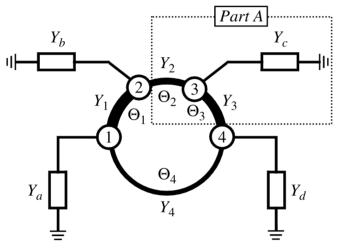
\includegraphics[width=0.5\textwidth]{../assets/review/ring_hybrid.pdf}
			\caption*{
				Fig. A 4-port asymmetric ring hybrid. Here the arc length between ports are $\Theta_1 = \Theta_2 = \Theta_3 = \lambda / 4$ and $\Theta_4 = 3 \lambda / 4$ where $\lambda$ is the wavelength. The termination admittances $Y_a$ to $Y_d$ are arbitrary and the characteristic admittances of transmission-line sections are not necessarily the same, such that the scattering parameters can be asymmetric. Source: modified from \cite{Ahn2006}.
			}
		\end{figure}

		On the other hand, symmetric \gls{ris} satisfying $\mathbf{\Theta} = \mathbf{\Theta}^\mathsf{T}$ are often considered in the literature as they can be implemented with simpler circuit components (e.g., capacitors and inductors).
		We have added Section \ref{sc:ris_symmetry} to investigate the impact of \gls{ris} symmetry on the system performance.

		\change{
			Symmetric \gls{ris} satisfying $\mathbf{\Theta} = \mathbf{\Theta}^\mathsf{T}$ are often considered in the literature due to hardware constraints.
			This study aim to investigate the impact of \gls{ris} symmetry on the system performance.
			\begin{remark}
				All proposed asymmetric \gls{bd}-\gls{ris} designs can be modified for symmetry. In particular,
				\begin{enumerate}[label=(\roman*)]
					\item \emph{\gls{svd}-based (e.g., \eqref{eq:ris_nd_sv_indl}, \eqref{eq:ris_nd_power}, \eqref{eq:ris_nd_rate_max}, \eqref{eq:ris_power}, \eqref{eq:ris_procrustes}):} Those closed-form asymmetric solutions are constructed from the product of singular matrices. If symmetry is required, one can replace the $\mathbf{U}, \mathbf{V}$ from the \gls{svd} of $\mathbf{A} = \mathbf{U} \mathbf{\Sigma} \mathbf{V}^\mathsf{H}$ by the factor $\mathbf{Q}$ from the Autonne-Takagi factorization of $\frac{\mathbf{A} + \mathbf{A}^\mathsf{T}}{2} = \mathbf{Q} \mathbf{\Sigma} \mathbf{Q}^\mathsf{T}$ \cite{Ikramov2012} to construct the corresponding $\mathbf{\Theta}$;
					\item \emph{\gls{rcg}-based (e.g., \eqref{eq:shaping_subdiff}, \eqref{eq:gradient_eucl_rate}):} The symmetry constraint is added to the corresponding optimization problems, and one can project the solution to the nearest symmetric point $\mathbf{\Theta} \gets \frac{\mathbf{\Theta} + \mathbf{\Theta}^\mathsf{T}}{2}$ after each iteration.
				\end{enumerate}
			\end{remark}

			\begin{figure}[H]
				\centering
				\subfloat[Power: $2 \times N_\mathrm{S} \times 2$]{
					\resizebox{!}{5cm}{
						% This file was created by matlab2tikz.
%
%The latest updates can be retrieved from
%  http://www.mathworks.com/matlabcentral/fileexchange/22022-matlab2tikz-matlab2tikz
%where you can also make suggestions and rate matlab2tikz.
%
\definecolor{mycolor1}{rgb}{0.00000,0.44706,0.74118}%
\definecolor{mycolor2}{rgb}{0.85098,0.32549,0.09804}%
%
\begin{tikzpicture}

\begin{axis}[%
width=9.509cm,
height=7.5cm,
at={(0cm,0cm)},
scale only axis,
xmin=1,
xmax=7,
xtick={1,2,3,4,5,6,7},
xticklabels={{$2^0$},{$2^1$},{$2^2$},{$2^3$},{$2^4$},{$2^5$},{$2^6$}},
% xlabel style={font=\color{white!15!black}},
xlabel={RIS Group Size},
ymin=0,
ymax=9e-07,
% ylabel style={font=\color{white!15!black}},
ylabel={Channel Power [W]},
axis background/.style={fill=white},
xmajorgrids,
ymajorgrids,
legend style={at={(0.03,0.97)}, anchor=north west, legend cell align=left, align=left, draw=white!15!black}
]
\addplot [color=mycolor1, line width=2.0pt, mark=o, mark options={solid, mycolor1}]
  table[row sep=crcr]{%
1	3.07226159314351e-08\\
2	4.11492399332381e-08\\
3	4.88148530601955e-08\\
4	5.26094766034717e-08\\
5	5.43186358023285e-08\\
};
\addlegendentry{Asymmetric: $N_\mathrm{S} = 16$}

\addplot [color=mycolor1, dashed, line width=2.0pt, mark=o, mark options={solid, mycolor1}]
  table[row sep=crcr]{%
1	3.07226159314351e-08\\
2	2.48110921829919e-08\\
3	2.09999716084868e-08\\
4	1.85392359072275e-08\\
5	1.69392170352418e-08\\
};
\addlegendentry{Enforced: $N_\mathrm{S} = 16$}

\addplot [color=mycolor1, dotted, line width=2.0pt, mark=o, mark options={solid, mycolor1}]
  table[row sep=crcr]{%
1	2.18823167401622e-08\\
2	2.58667252589526e-08\\
3	3.6393122841988e-08\\
4	4.41807731672663e-08\\
5	4.8483723780213e-08\\
};
\addlegendentry{Legacy: $N_\mathrm{S} = 16$}

\addplot [color=mycolor1, dashdotted, line width=2.0pt, mark=o, mark options={solid, mycolor1}]
  table[row sep=crcr]{%
1	3.07226159314351e-08\\
2	3.78824565046636e-08\\
3	4.6008649901077e-08\\
4	5.13929112888468e-08\\
5	5.39731769119744e-08\\
};
\addlegendentry{Takagi: $N_\mathrm{S} = 16$}

\addplot [color=mycolor2, line width=2.0pt, mark=+, mark options={solid, mycolor2}]
  table[row sep=crcr]{%
1	3.73674394477017e-07\\
2	5.420346500246e-07\\
3	6.85389992643681e-07\\
4	7.6227451113248e-07\\
5	8.0069480829595e-07\\
6	8.18206267524393e-07\\
7	8.25088677505729e-07\\
};
\addlegendentry{Asymmetric: $N_\mathrm{S} = 64$}

\addplot [color=mycolor2, dashed, line width=2.0pt, mark=+, mark options={solid, mycolor2}]
  table[row sep=crcr]{%
1	3.73674394477017e-07\\
2	3.06957520044884e-07\\
3	2.68618316241873e-07\\
4	2.45748953801729e-07\\
5	2.27807576071471e-07\\
6	2.22821968007804e-07\\
7	2.16970499497674e-07\\
};
\addlegendentry{Enforced: $N_\mathrm{S} = 64$}

\addplot [color=mycolor2, dotted, line width=2.0pt, mark=+, mark options={solid, mycolor2}]
  table[row sep=crcr]{%
1	3.02768340133104e-07\\
2	3.67874038919462e-07\\
3	5.47929160259681e-07\\
4	6.80081694767098e-07\\
5	7.48298918253076e-07\\
6	7.85561233493806e-07\\
7	8.04051669342744e-07\\
};
\addlegendentry{Legacy: $N_\mathrm{S} = 64$}

\addplot [color=mycolor2, dashdotted, line width=2.0pt, mark=+, mark options={solid, mycolor2}]
  table[row sep=crcr]{%
1	3.73674394477017e-07\\
2	4.73667276858297e-07\\
3	6.21291346950978e-07\\
4	7.28822615730252e-07\\
5	7.83509460162992e-07\\
6	8.10199796739281e-07\\
7	8.22445224822532e-07\\
};
\addlegendentry{Takagi: $N_\mathrm{S} = 64$}

\end{axis}
\end{tikzpicture}%

					}
				}
				\subfloat[Rate: $4 \times N_\mathrm{S} \times 4$]{
					\resizebox{!}{5cm}{
						% This file was created by matlab2tikz.
%
%The latest updates can be retrieved from
%  http://www.mathworks.com/matlabcentral/fileexchange/22022-matlab2tikz-matlab2tikz
%where you can also make suggestions and rate matlab2tikz.
%
\definecolor{mycolor1}{rgb}{0.00000,0.44706,0.74118}%
\definecolor{mycolor2}{rgb}{0.85098,0.32549,0.09804}%
%
\begin{tikzpicture}

\begin{axis}[%
width=11.411cm,
height=9cm,
at={(0cm,0cm)},
scale only axis,
xmin=-20,
xmax=20,
xlabel style={font=\color{white!15!black}},
xlabel={Transmit Power [dB]},
ymin=0,
ymax=60,
ylabel style={font=\color{white!15!black}},
ylabel={Achievable Rate [bit/s/Hz]},
axis background/.style={fill=white},
xmajorgrids,
ymajorgrids,
legend style={at={(0.03,0.97)}, anchor=north west, legend cell align=left, align=left, draw=white!15!black}
]
\addplot [color=black, line width=2.0pt]
  table[row sep=crcr]{%
-20	0.869712506220171\\
-15	2.11804892861715\\
-10	4.32580899488593\\
-5	7.87508759965494\\
0	12.6780205038048\\
5	18.1780871974283\\
10	24.328728256457\\
15	30.8030513368595\\
20	37.3917434238629\\
};
\addlegendentry{No RIS}

\addplot [color=mycolor1, line width=2.0pt, mark=o, mark options={solid, mycolor1}]
  table[row sep=crcr]{%
-20	1.05029082922333\\
-15	2.47337886006358\\
-10	4.92048529343925\\
-5	8.90477411631522\\
0	13.9570874291404\\
5	19.8957463831554\\
10	26.2933401587038\\
15	32.8565936354346\\
20	39.4746708507294\\
};
\addlegendentry{Asymmetric BD: $N_\mathrm{S} = 16$}

\addplot [color=mycolor1, dashed, line width=2.0pt, mark=o, mark options={solid, mycolor1}]
  table[row sep=crcr]{%
-20	0.970760076661331\\
-15	2.3188320234014\\
-10	4.64280739162619\\
-5	8.41835694674129\\
0	13.3604486433245\\
5	19.094165557721\\
10	25.4186344249109\\
15	31.9565133951396\\
20	38.5663724097166\\
};
\addlegendentry{Symmetric-Enforced BD: $N_\mathrm{S} = 16$}

\addplot [color=mycolor1, dotted, line width=2.0pt, mark=o, mark options={solid, mycolor1}]
  table[row sep=crcr]{%
-20	0.97597456292552\\
-15	2.30584921620253\\
-10	4.62292261488193\\
-5	8.33348997224921\\
0	13.3557952177725\\
5	18.9906847997489\\
10	25.437800763079\\
15	31.9385728892858\\
20	38.5311499513319\\
};
\addlegendentry{Symmetric-Projected BD: $N_\mathrm{S} = 16$}

\addplot [color=mycolor2, line width=2.0pt, mark=+, mark options={solid, mycolor2}]
  table[row sep=crcr]{%
-20	3.77847987240857\\
-15	6.50928071370314\\
-10	12.1387730745713\\
-5	18.5875271015713\\
0	24.3077905361749\\
5	33.2971078250378\\
10	39.928680684664\\
15	46.5685472744417\\
20	53.211140381742\\
};
\addlegendentry{Asymmetric BD: $N_\mathrm{S} = 256$}

\addplot [color=mycolor2, dashed, line width=2.0pt, mark=+, mark options={solid, mycolor2}]
  table[row sep=crcr]{%
-20	2.34847395704067\\
-15	4.62061866587552\\
-10	8.87596224335232\\
-5	14.477655849128\\
0	20.072194318481\\
5	28.1693217002636\\
10	34.7805310048903\\
15	41.4138537995477\\
20	48.0542910369292\\
};
\addlegendentry{Symmetric-Enforced BD: $N_\mathrm{S} = 256$}

\addplot [color=mycolor2, dotted, line width=2.0pt, mark=+, mark options={solid, mycolor2}]
  table[row sep=crcr]{%
-20	2.56771808601858\\
-15	4.62163031351707\\
-10	9.02266665728213\\
-5	15.8352879313011\\
0	20.2736387755067\\
5	29.3911431192357\\
10	35.1742881633618\\
15	43.1166685548033\\
20	49.7257139129898\\
};
\addlegendentry{Symmetric-Projected BD: $N_\mathrm{S} = 256$}

\end{axis}
\end{tikzpicture}%
					}
				}
				\caption*{
					Fig. Impact of \gls{ris} symmetry on the power gain and achievable rate of \gls{mimo} point-to-point channel.
				}
			\end{figure}

			Figs. \ref{fg:pc_power_symmetry} and \ref{fg:pc_rate_symmetry} compare the power gain and achievable rate of \gls{mimo} point-to-point channel under asymmetric and various symmetric \gls{ris} configurations.
			Here, `Asymmetric' refers to the benchmark solution by \eqref{eq:ris_power} or \eqref{eq:gradient_eucl_rate}, `Enforced' refers to enforcing symmetry on `Asymmetric', `Legacy' refers to a straightforward extension of the \gls{siso} \gls{snr}-optimal solution \cite[(6)]{Santamaria2023}, `Takagi' refers to the modification \ref{it:takagi}, and `Projection' refers to the modification \ref{it:projection}.
			We observe that the performance gaps between the asymmetric and symmetric \gls{ris} configurations are insignificant and tends to widen with the number of scattering elements.
			The two proposed modifications also outperform other candidates in both problems.
		}
	}

	\comment{
		The geodesic \gls{rcg} method seems promising especially at large group size $L$. Is it possible to extend the design framework to advanced \gls{bd}-\gls{ris} architectures (e.g., multi-sector mode)?
	}

	\reply{
		Unfortunately, the geodesic \gls{rcg} method relies on the block unitary property of the \gls{bd}-\gls{ris} scattering matrix and is not directly applicable to multi-sector mode \gls{bd}-\gls{ris} where the constraint is relaxed to $\sum_{s=1}^S \mathbf{\Theta}_{g,s}^\mathsf{H} \mathbf{\Theta}_{g,s} = \mathbf{I}, \ \forall g \in [G]$ with $S > 1$ sectors.
	}

	\comment{
		For fully-connected \gls{bd}-\gls{ris}, the authors mentioned in the result section that power gain-optimal scattering matrix is also rate-optimal. Can you provide a proof on this point?
	}

	\reply{
		This is truly an interesting observation.
		When the direct channel is negligible and \gls{bd}-\gls{ris} is fully-connected, the power gain-optimal and rate-optimal scattering matrices derived in closed form \eqref{eq:ris_nd_power_max} and \eqref{eq:ris_nd_rate_max} indeed coincide with each other.
		When the direct channel is significant, the observation still holds, yet we do not have a formal proof due to the non-trivial solution structures.
		The following context has been added to the manuscript to support this claim.

		\change{
			Corollary \ref{co:nd_capacity_snr_general} also suggests that the power- and rate-optimal scattering matrices \eqref{eq:ris_nd_power_max} and \eqref{eq:ris_nd_rate_max} coincide with each other when the direct channel is negligible and the \gls{bd}-\gls{ris} is fully-connected.
			When either condition is not satisfied, active and passive beamforming are coupled and the rate-optimal solution involves alternating optimization.
			However, the power gain-optimal \gls{ris} still provides for a low-complexity decoupled solution.
		}
		\change{
			We also see that for fully-connected \gls{bd}-\gls{ris}, the power gain-optimal and rate-optimal points coincide with each other, as derived in  \eqref{eq:ris_nd_power_max} and \eqref{eq:ris_nd_rate_max}.
			This observation still holds in Figs. \subref*{fg:singular_pareto_sx32} -- \subref*{fg:singular_pareto_sx128} where the direct channel is significant, yet a formal proof is unavailable due to the non-trivial solution structures.
		}
	}

	\comment{
		The authors refer to \cite{Li2024} for estimating forward and backward channels individually. However, it can be challenging to implement those in real time without RF chains at the \gls{ris}. The impact of imperfect \gls{csi} on the achievable rates may also be studied.
	}

	\reply{
		We agree with the reviewer that the estimation of individual forward and backward channels may be challenging in practice.
		Section \ref{sc:estimation_error} has been added to investigate the impact of imperfect \gls{csi} on the proposed beamforming designs.

		\change{
			\begin{figure}[H]
				\centering
				\subfloat[Pareto: $2 \times 64 \times 2$]{
					\resizebox{!}{3.15cm}{
						% This file was created by matlab2tikz.
%
%The latest updates can be retrieved from
%  http://www.mathworks.com/matlabcentral/fileexchange/22022-matlab2tikz-matlab2tikz
%where you can also make suggestions and rate matlab2tikz.
%
\definecolor{mycolor1}{rgb}{0.00000,0.44700,0.74100}%
\definecolor{mycolor2}{rgb}{0.92900,0.69400,0.12500}%
\definecolor{mycolor3}{rgb}{0.49400,0.18400,0.55600}%
\definecolor{mycolor4}{rgb}{0.63500,0.07800,0.18400}%
\definecolor{mycolor5}{rgb}{0.46600,0.67400,0.18800}%
\definecolor{mycolor6}{rgb}{0.85000,0.32500,0.09800}%
\definecolor{mycolor7}{rgb}{0.30100,0.74500,0.93300}%
\definecolor{mycolor8}{rgb}{0.50196,0.50196,0.50196}%
%
\begin{tikzpicture}

\begin{axis}[%
width=9.509cm,
height=7.5cm,
at={(0cm,0cm)},
scale only axis,
unbounded coords=jump,
xmin=0.000292357955879774,
xmax=0.00146931598006191,
% xlabel style={font=\color{white!15!black}},
xlabel={$\sigma_1(\mathbf{H})$},
ymin=5.00353872452725e-07,
ymax=0.000855139152254738,
% ylabel style={font=\color{white!15!black}},
ylabel={$\sigma_2(\mathbf{H})$},
axis background/.style={fill=white},
xmajorgrids,
ymajorgrids,
legend style={at={(0.03,0.97)}, anchor=north west, legend cell align=left, align=left, draw=white!15!black},
every axis plot/.append style={line width=1.5pt}
]
\addplot[only marks, mark=triangle, mark options={}, mark size=4pt, draw=black] table[row sep=crcr]{%
x	y\\
0.000839165048501169	0.000214263316833017\\
};
\addlegendentry{Direct}

\addplot [color=mycolor1, dashed, line width=3.0pt]
  table[row sep=crcr]{%
0.00120932633718953	0.000583119017598987\\
0.00119575201720946	0.000596081239213197\\
0.00117726551646851	0.000611861101174529\\
0.00116606299082248	0.000620580102997392\\
0.00115424592284094	0.000628870538828447\\
0.00113886771388772	0.000638539772491746\\
0.00111898950928878	0.000649774010006312\\
0.00110183012413076	0.000658373581049715\\
0.00108325437257282	0.000666566528121604\\
0.001063768616969	0.000673393058199169\\
0.00104157703419366	0.000680312749731737\\
0.00102940704848264	0.000683655627075032\\
0.00101534590489402	0.000686767298208718\\
0.0010026917822706	0.000688974641564217\\
0.00099097088499458	0.000690411158545693\\
0.000975869339018042	0.000691490294174907\\
0.00096019933715482	0.000691860001599399\\
0.000944270055421307	0.000691427925266965\\
0.000923381543260725	0.000689880173702533\\
0.000906338430168291	0.000687778553566788\\
0.000890771657779231	0.000685055092600335\\
0.000874967807227278	0.000681494832282678\\
0.000860651531189936	0.000677538166163577\\
0.00084263466302954	0.000671530981556631\\
0.000833179943934603	0.000667891247037841\\
0.000825096636366874	0.00066430463113554\\
0.000817622286439315	0.000660533145039521\\
0.000810229737161579	0.000656334038054984\\
0.000802689225471437	0.000651563607280594\\
0.000797565212369227	0.000648027775864695\\
0.00079153891940423	0.00064351105664721\\
0.000784321813851128	0.000637592054903147\\
0.000777733164379927	0.000631712159747391\\
0.000441524298685212	0.000296037981911999\\
0.000434469809806145	0.00028814322809853\\
0.000428092651889828	0.000280170072109908\\
0.000422631513802745	0.000272581400590931\\
0.000417648726184689	0.000264924313108306\\
0.000412471420119124	0.000256109633332169\\
0.000407648973867364	0.000246885310746728\\
0.000403028531630567	0.000236849224421848\\
0.000398822264577218	0.000226476405700697\\
0.000394233101548728	0.000213511948147064\\
0.000390225450359751	0.000200091453867316\\
0.000386614485758307	0.000185348027264666\\
0.000383675555943931	0.000170337808639181\\
0.000380968519648806	0.000151900607665391\\
0.000379059275924778	0.000132622462208425\\
0.000378194792996519	0.000114943948967252\\
0.000378226418735324	9.89468700138412e-05\\
0.000378884085713094	8.62508167801333e-05\\
0.000380569640365825	7.03420220286831e-05\\
0.00038618679753343	3.2704930777993e-05\\
0.000392139965165464	1.76545987441939e-05\\
0.000398143101171136	4.42592319687909e-06\\
0.000400015585409934	7.84639312588013e-07\\
0.000400890956764154	5.36547173317211e-07\\
0.000401760254197925	5.01004440513917e-07\\
0.000401781864355714	5.00353872452725e-07\\
0.00130733817970372	1.04917083605326e-06\\
0.00130733817970373	1.04917083605349e-06\\
0.00130733824343437	1.04934572103263e-06\\
0.00131566404537624	2.75924910873365e-05\\
0.00132002132522115	4.31868231132689e-05\\
0.00132362706051804	5.93309503755032e-05\\
0.00132807382278624	8.4683899850467e-05\\
0.00133195793694021	0.000116308252543656\\
0.00133439025321267	0.000150391916544675\\
0.001335396584083	0.000193411167999653\\
0.00133390666371673	0.000252240584333186\\
0.00133056020206507	0.000297825772154749\\
0.00132669877840738	0.000329091629685837\\
0.00132209572955983	0.000355429694817544\\
0.00131557906744292	0.000384322067807563\\
0.00130856007339145	0.000409670350270726\\
0.00130092669810398	0.000432619438275947\\
0.00128961290453414	0.000461695061770904\\
0.00127993906730125	0.000483570717832979\\
0.00127155738904107	0.000500166508701635\\
0.0012630999277564	0.000515008980512333\\
0.00125414139085769	0.000529062388896712\\
0.00124447591477809	0.000542698501702921\\
0.00123400340183044	0.000556039848291126\\
0.001222422875848	0.000569395636875488\\
0.00120932633718953	0.000583119017598987\\
};
\addlegendentry{D: $\epsilon = 0.01$}

\addplot[only marks, mark=o, mark options={}, mark size=5pt, draw=mycolor1, forget plot] table[row sep=crcr]{%
x	y\\
0.00130856007339145	0.000409670350270726\\
};
\addplot[only marks, mark=x, mark options={}, mark size=5pt, draw=mycolor1, forget plot] table[row sep=crcr]{%
x	y\\
0.001335396584083	0.000193411167999653\\
};
\addplot [color=mycolor1, line width=3.0pt, forget plot]
  table[row sep=crcr]{%
0.001335396584083	0.000193411167999653\\
0.00133390666371673	0.000252240584333186\\
0.00133056020206507	0.000297825772154749\\
0.00132669877840738	0.000329091629685837\\
0.00132209572955983	0.000355429694817544\\
0.00131557906744292	0.000384322067807563\\
0.00130856007339145	0.000409670350270726\\
0.00130092669810398	0.000432619438275947\\
0.00128961290453414	0.000461695061770904\\
0.00127993906730125	0.000483570717832979\\
0.00127155738904107	0.000500166508701635\\
0.0012630999277564	0.000515008980512333\\
0.00125414139085769	0.000529062388896712\\
0.00124447591477809	0.000542698501702921\\
0.00123400340183044	0.000556039848291126\\
0.001222422875848	0.000569395636875488\\
0.00120932633718953	0.000583119017598987\\
0.00120932633718953	0.000583119017598987\\
0.00119575201720946	0.000596081239213197\\
0.00117726551646851	0.000611861101174529\\
0.00116606299082248	0.000620580102997392\\
0.00115424592284094	0.000628870538828447\\
0.00113886771388772	0.000638539772491746\\
0.00111898950928878	0.000649774010006312\\
0.00110183012413076	0.000658373581049715\\
0.00108325437257282	0.000666566528121604\\
0.001063768616969	0.000673393058199169\\
0.00104157703419366	0.000680312749731737\\
0.00102940704848264	0.000683655627075032\\
0.00101534590489402	0.000686767298208718\\
0.0010026917822706	0.000688974641564217\\
0.00099097088499458	0.000690411158545693\\
0.000975869339018042	0.000691490294174907\\
0.00096019933715482	0.000691860001599399\\
};
\addplot [opacity=0.667, color=mycolor1, dashed, line width=3.0pt]
  table[row sep=crcr]{%
0.00120723012416074	0.000580649381500933\\
0.00119572729949016	0.000591745547210129\\
0.00118323402865883	0.000602798267829881\\
0.00117091537169704	0.000612839661119823\\
0.00115871195379311	0.000621853409700489\\
0.00114557630666833	0.000630548168328466\\
0.00112381067899623	0.000643396496125846\\
0.00110490865706361	0.00065352458175076\\
0.00108323062533875	0.00066324307023993\\
0.00105217157633789	0.000674306046892957\\
0.00103852102435755	0.00067826603848561\\
0.00102662790265939	0.000681104564886569\\
0.00101556058282178	0.00068328724779443\\
0.00100435117234784	0.000685068812689737\\
0.000992864015068341	0.000686406907038555\\
0.000979441788478403	0.000687342785378085\\
0.000963855285803246	0.000687717102169256\\
0.000948058830893159	0.000687280169509713\\
0.00092940877843491	0.000685885826937215\\
0.000911571441685017	0.000683711468008641\\
0.000894387573610684	0.000680699586104162\\
0.000877435937001939	0.000676840186873352\\
0.000857390104973841	0.000670820436095137\\
0.000846247012304084	0.000667074354965531\\
0.00083702695229735	0.000663404368656974\\
0.000828405618219941	0.000659373359582414\\
0.000820307528666392	0.000655058369952753\\
0.000813154779696064	0.000650847743907278\\
0.000806694137532323	0.000646665605428428\\
0.000802863701419803	0.00064400843587972\\
0.000797548426269461	0.00064002686775209\\
0.000791726365677255	0.000635281026831634\\
0.000785241970194614	0.000629484141544239\\
0.000450253072269392	0.000295130453124787\\
0.000443925306443406	0.000288248687422809\\
0.000437864912868001	0.000280935921502853\\
0.000432334917526517	0.000273476743656745\\
0.0004261872727151	0.000264332926337528\\
0.000420776171850977	0.000255147287321726\\
0.000415063280504114	0.000244224441864073\\
0.000411023454093519	0.000235210593730386\\
0.000406472971950957	0.000222764293180299\\
0.000401019635746126	0.000207189977302398\\
0.00039697662692898	0.000193114474755604\\
0.000393733215238289	0.000179239481115576\\
0.000391058369075111	0.000165112158252769\\
0.000388549264458002	0.000147975470967991\\
0.000386780242306876	0.000129368296321085\\
0.000386065682272045	0.00011437207647525\\
0.000386038743317747	0.000101193805734313\\
0.000386569086633482	8.84784721748764e-05\\
0.00038764069524001	7.63670297314887e-05\\
0.000392923494859776	3.45641459698829e-05\\
0.000396450893267522	1.65206667761283e-05\\
0.000398597614915704	1.00099888062855e-05\\
0.000400336315289976	7.24206559109498e-06\\
0.000402653082589453	6.26178688962721e-06\\
0.000402717796617414	6.23904507595133e-06\\
0.000402717796617414	6.2390450759513e-06\\
0.000583868021978105	5.43299949955658e-06\\
0.00130375716626679	6.79156794051234e-06\\
0.0013041937899189	7.84000214723081e-06\\
0.00131228500208719	3.40132985725704e-05\\
0.00131624094647624	4.86094735783491e-05\\
0.00131969258780504	6.43480463589392e-05\\
0.00132317871828661	8.44959404070106e-05\\
0.00132773748084538	0.000115724237911933\\
0.00133001746507462	0.000142934636115753\\
0.00133088767352632	0.000186670530727628\\
0.00133017374050803	0.000247743221422876\\
0.00132773744729883	0.000287931387759637\\
0.00132422561125768	0.000320204358037492\\
0.00131943435417675	0.000349507358963146\\
0.00131329985055898	0.000378000486951702\\
0.00130676080816937	0.000402926442904334\\
0.00129953974025189	0.000425922991478535\\
0.00129055003033978	0.000450226741951118\\
0.00128057806813479	0.000473892662606403\\
0.00127142153795021	0.000493134650385841\\
0.00126268033911301	0.000509168626837649\\
0.00125350499759553	0.000524077981137843\\
0.00124378686109559	0.000538195569220947\\
0.00123312164972066	0.000552094566569883\\
0.00121990237114162	0.000567381051703403\\
0.00120723012416074	0.000580649381500933\\
};
\addlegendentry{D: $\epsilon = 0.1$}

\addplot[opacity=0.667, only marks, mark=o, mark options={}, mark size=5pt, draw=mycolor1, forget plot] table[row sep=crcr]{%
x	y\\
0.00129953974025189	0.000425922991478535\\
};
\addplot[opacity=0.667, only marks, mark=x, mark options={}, mark size=5pt, draw=mycolor1, forget plot] table[row sep=crcr]{%
x	y\\
0.00133088767352632	0.000186670530727628\\
};
\addplot [opacity=0.667, color=mycolor1, line width=3.0pt, forget plot]
  table[row sep=crcr]{%
0.00133088767352632	0.000186670530727628\\
0.00133017374050803	0.000247743221422876\\
0.00132773744729883	0.000287931387759637\\
0.00132422561125768	0.000320204358037492\\
0.00131943435417675	0.000349507358963146\\
0.00131329985055898	0.000378000486951702\\
0.00130676080816937	0.000402926442904334\\
0.00129953974025189	0.000425922991478535\\
0.00129055003033978	0.000450226741951118\\
0.00128057806813479	0.000473892662606403\\
0.00127142153795021	0.000493134650385841\\
0.00126268033911301	0.000509168626837649\\
0.00125350499759553	0.000524077981137843\\
0.00124378686109559	0.000538195569220947\\
0.00123312164972066	0.000552094566569883\\
0.00121990237114162	0.000567381051703403\\
0.00120723012416074	0.000580649381500933\\
0.00120723012416074	0.000580649381500933\\
0.00119572729949016	0.000591745547210129\\
0.00118323402865883	0.000602798267829881\\
0.00117091537169704	0.000612839661119823\\
0.00115871195379311	0.000621853409700489\\
0.00114557630666833	0.000630548168328466\\
0.00112381067899623	0.000643396496125846\\
0.00110490865706361	0.00065352458175076\\
0.00108323062533875	0.00066324307023993\\
0.00105217157633789	0.000674306046892957\\
0.00103852102435755	0.00067826603848561\\
0.00102662790265939	0.000681104564886569\\
0.00101556058282178	0.00068328724779443\\
0.00100435117234784	0.000685068812689737\\
0.000992864015068341	0.000686406907038555\\
0.000979441788478403	0.000687342785378085\\
0.000963855285803246	0.000687717102169256\\
};
\addplot [opacity=0.333, color=mycolor1, dashed, line width=3.0pt]
  table[row sep=crcr]{%
0.00110722127930191	0.00055231862569117\\
0.0010950603254174	0.00055964768047213\\
0.00108547410172965	0.00056526768014669\\
0.00108090453727743	0.000567824281317283\\
0.00107660910789735	0.000569850547760194\\
0.00107229143829399	0.000571622340327614\\
0.00106773267965282	0.000573279032414328\\
0.00106256311230578	0.000574969360498219\\
0.00104784919952727	0.000579469887650121\\
0.00103874039558323	0.000581995247615636\\
0.00102883599392078	0.00058367868645446\\
0.00101819521148904	0.000584080812793491\\
0.000978855415163161	0.000583380406652782\\
0.000928523427871111	0.000580022438230062\\
0.000917984747042123	0.000578929961136174\\
0.000908304406902503	0.000577464606670763\\
0.000899104704584145	0.000575636018707832\\
0.000890493529967113	0.00057352492657437\\
0.000882601773118892	0.000571207663249651\\
0.00087535130087042	0.000568686253554518\\
0.000868517872535676	0.000565888024055649\\
0.000861873785990023	0.000562710633228406\\
0.000855280934632879	0.000559088933603478\\
0.000848716167899615	0.000555044826053949\\
0.000838296885173201	0.000548097883356892\\
0.00083284725164066	0.000544123720530958\\
0.000827369422440948	0.000539643693075147\\
0.000522389860125143	0.000288044812067282\\
0.000516516721686327	0.000281285041617264\\
0.000510684009963046	0.000273400693690491\\
0.000505000957031184	0.000264800118145228\\
0.000499359074801272	0.000255419148656063\\
0.000494439072797046	0.000245427354342094\\
0.000489286065066436	0.000234699824553598\\
0.000483329731374156	0.000221903685132653\\
0.000477640370699273	0.000207987936565\\
0.000471857300041654	0.000191090776375776\\
0.000468005947815214	0.000175452431539676\\
0.000466258026820786	0.000162539849289817\\
0.000464878489647416	0.00015071779912929\\
0.000463932838780443	0.000138354327627574\\
0.000463209986977303	0.000126711524489337\\
0.000463045849092032	0.00011421695454841\\
0.000464076147870395	9.72894347089132e-05\\
0.000466126418233955	7.278474756215e-05\\
0.000467747387169956	6.79953909667504e-05\\
0.000619547044543305	6.21542263318127e-05\\
0.00124921683817881	9.27965760077673e-05\\
0.00124921683817882	9.27965760077696e-05\\
0.00125061928271792	9.74490799027226e-05\\
0.00126064627294896	0.000137492920950342\\
0.00126207053113663	0.000148633952727836\\
0.00126268994822494	0.000157880740079037\\
0.001262775195004	0.000181063828595574\\
0.00125962161650267	0.000229932308940695\\
0.00125507144106471	0.000273174115566032\\
0.00125051881218205	0.000311623680125553\\
0.00124051948090657	0.000347659681552022\\
0.00123385608693869	0.000371317295327494\\
0.00122748631434108	0.000393853984872361\\
0.00121944327786394	0.000415934092633447\\
0.00121040506725937	0.000435820712044041\\
0.00118962404774373	0.000476528980532702\\
0.00118085669557352	0.000487935282336488\\
0.00117183625322355	0.000498471436893667\\
0.00116256638850969	0.000508203035476104\\
0.00115302695345452	0.000517222822417311\\
0.00114299471484386	0.000525809792659205\\
0.0011317939784689	0.000534311032065687\\
0.00110722127930191	0.00055231862569117\\
};
\addlegendentry{D: $\epsilon = 0.5$}

\addplot[opacity=0.333, only marks, mark=o, mark options={}, mark size=5pt, draw=mycolor1, forget plot] table[row sep=crcr]{%
x	y\\
0.00122748631434108	0.000393853984872361\\
};
\addplot[opacity=0.333, only marks, mark=x, mark options={}, mark size=5pt, draw=mycolor1, forget plot] table[row sep=crcr]{%
x	y\\
0.001262775195004	0.000181063828595574\\
};
\addplot [opacity=0.333, color=mycolor1, line width=3.0pt, forget plot]
  table[row sep=crcr]{%
0.001262775195004	0.000181063828595574\\
0.00125962161650267	0.000229932308940695\\
0.00125507144106471	0.000273174115566032\\
0.00125051881218205	0.000311623680125553\\
0.00124051948090657	0.000347659681552022\\
0.00123385608693869	0.000371317295327494\\
0.00122748631434108	0.000393853984872361\\
0.00121944327786394	0.000415934092633447\\
0.00121040506725937	0.000435820712044041\\
0.00118962404774373	0.000476528980532702\\
0.00118085669557352	0.000487935282336488\\
0.00117183625322355	0.000498471436893667\\
0.00116256638850969	0.000508203035476104\\
0.00115302695345452	0.000517222822417311\\
0.00114299471484386	0.000525809792659205\\
0.0011317939784689	0.000534311032065687\\
0.00110722127930191	0.00055231862569117\\
0.00110722127930191	0.00055231862569117\\
0.0010950603254174	0.00055964768047213\\
0.00108547410172965	0.00056526768014669\\
0.00108090453727743	0.000567824281317283\\
0.00107660910789735	0.000569850547760194\\
0.00107229143829399	0.000571622340327614\\
0.00106773267965282	0.000573279032414328\\
0.00106256311230578	0.000574969360498219\\
0.00104784919952727	0.000579469887650121\\
0.00103874039558323	0.000581995247615636\\
0.00102883599392078	0.00058367868645446\\
0.00101819521148904	0.000584080812793491\\
};
\addplot [color=mycolor6, dashed, line width=3.0pt]
  table[row sep=crcr]{%
0.00146681015044238	0.000852691160218086\\
0.00146655353540688	0.00085293323578946\\
0.0014662843547074	0.000853162890053388\\
0.0014659999443247	0.000853382058906823\\
0.00146569873492164	0.000853591142986456\\
0.00146537786977228	0.000853790987445657\\
0.00146503583744612	0.000853981103932059\\
0.00146466901723951	0.000854161789887561\\
0.00146427408817534	0.000854332555068325\\
0.00146384588816425	0.000854493022963016\\
0.00146338001330438	0.000854641789717379\\
0.00146286837965225	0.000854777647926877\\
0.00146230537852938	0.00085489776865824\\
0.0014616804308002	0.000854999222340005\\
0.00146098104619341	0.000855077662321666\\
0.00146019189894725	0.000855127076148748\\
0.00145929133993952	0.000855139152254738\\
0.000856795082982419	0.000854198016477824\\
0.000856109717751413	0.000853761150395599\\
0.000292531578686958	0.000291275356291254\\
0.0002924996535061	0.000289286117898126\\
0.000292468450754768	0.000276170063242794\\
0.000292438505603605	0.000227020923484573\\
0.000292357955879774	9.57693921944774e-07\\
0.00029235864001388	9.52452028573311e-07\\
0.000292359025324758	9.51243212844082e-07\\
0.00146795919069224	9.55327674380309e-07\\
0.00146795919069226	9.55327676142196e-07\\
0.00146931598006191	0.0008451691026365\\
0.00146929838454492	0.0008460739359627\\
0.00146924392219391	0.000846865155314428\\
0.00146916024584968	0.000847570100281123\\
0.00146905402164446	0.000848197473863468\\
0.00146892945901967	0.000848761721462629\\
0.00146878894868572	0.000849275354436091\\
0.0014686366705857	0.000849740048392178\\
0.00146847258403339	0.000850167769688045\\
0.00146829824275695	0.000850562344129948\\
0.0014681144525415	0.000850927976096036\\
0.00146792126731962	0.000851268890999304\\
0.00146771877116984	0.000851588066033354\\
0.0014675065123188	0.000851888384961548\\
0.00146728443410782	0.000852171497358568\\
0.00146705226525215	0.000852438856716109\\
0.00146681015044238	0.000852691160218086\\
};
\addlegendentry{BD: $\epsilon = 0.01$}

\addplot[only marks, mark=o, mark options={}, mark size=5pt, draw=mycolor6, forget plot] table[row sep=crcr]{%
x	y\\
0.00146792126731962	0.000851268890999304\\
};
\addplot[only marks, mark=x, mark options={}, mark size=5pt, draw=mycolor6, forget plot] table[row sep=crcr]{%
x	y\\
0.00146931598006191	0.0008451691026365\\
};
\addplot [color=mycolor6, line width=3.0pt, forget plot]
  table[row sep=crcr]{%
0.00146931598006191	0.0008451691026365\\
0.00146929838454492	0.0008460739359627\\
0.00146924392219391	0.000846865155314428\\
0.00146916024584968	0.000847570100281123\\
0.00146905402164446	0.000848197473863468\\
0.00146892945901967	0.000848761721462629\\
0.00146878894868572	0.000849275354436091\\
0.0014686366705857	0.000849740048392178\\
0.00146847258403339	0.000850167769688045\\
0.00146829824275695	0.000850562344129948\\
0.0014681144525415	0.000850927976096036\\
0.00146792126731962	0.000851268890999304\\
0.00146771877116984	0.000851588066033354\\
0.0014675065123188	0.000851888384961548\\
0.00146728443410782	0.000852171497358568\\
0.00146705226525215	0.000852438856716109\\
0.00146681015044238	0.000852691160218086\\
0.00146681015044238	0.000852691160218086\\
0.00146655353540688	0.00085293323578946\\
0.0014662843547074	0.000853162890053388\\
0.0014659999443247	0.000853382058906823\\
0.00146569873492164	0.000853591142986456\\
0.00146537786977228	0.000853790987445657\\
0.00146503583744612	0.000853981103932059\\
0.00146466901723951	0.000854161789887561\\
0.00146427408817534	0.000854332555068325\\
0.00146384588816425	0.000854493022963016\\
0.00146338001330438	0.000854641789717379\\
0.00146286837965225	0.000854777647926877\\
0.00146230537852938	0.00085489776865824\\
0.0014616804308002	0.000854999222340005\\
0.00146098104619341	0.000855077662321666\\
0.00146019189894725	0.000855127076148748\\
0.00145929133993952	0.000855139152254738\\
};
\addplot [opacity=0.667, color=mycolor6, dashed, line width=3.0pt]
  table[row sep=crcr]{%
0.00146121897207338	0.000846827535506497\\
0.00146097765394714	0.000847093950333192\\
0.00146072046558346	0.000847349487981516\\
0.00146044705057326	0.000847593672832021\\
0.00146015295046338	0.000847829260305024\\
0.00145983984942792	0.00084805325977882\\
0.0014595016939962	0.000848268353081352\\
0.00145913578163398	0.000848473809334482\\
0.00145873840121968	0.000848668898667813\\
0.00145830335024085	0.000848853209029696\\
0.00145782476309251	0.000849025106697699\\
0.00145729589640998	0.000849182402819355\\
0.00145670791857563	0.000849322132240472\\
0.0014560479376686	0.000849440501948768\\
0.00145530203038965	0.0008495318649295\\
0.00145445094325694	0.000849588684928226\\
0.00145347019769869	0.000849599956138923\\
0.00133535335023838	0.000848240585528493\\
0.000868558167512083	0.000842095233310384\\
0.000866006660522284	0.000840906431925238\\
0.000311204945422966	0.00028812611563894\\
0.000311163087059558	0.000288044007182338\\
0.00031111082767997	0.000287833840332238\\
0.000311022244068098	0.000287458393185244\\
0.000310178176636716	0.000281089953418288\\
0.000309037951403639	0.000259394766574548\\
0.000308547163468215	0.000218529816751153\\
0.000308135644918699	1.27562202441757e-05\\
0.000308142198405789	1.27543574073415e-05\\
0.0014514285412979	5.4934140812153e-06\\
0.00146253957895156	0.000392187410298758\\
0.00146316630554445	0.000637569357669725\\
0.00146329060060681	0.000839879224266291\\
0.00146327594387066	0.000840688293975485\\
0.00146323112408763	0.000841405744344246\\
0.00146316188308265	0.000842049058368922\\
0.00146307186276867	0.000842635311505379\\
0.00146296449834791	0.00084316902514609\\
0.00146284315951209	0.000843656449710219\\
0.0014627089825723	0.000844105394094888\\
0.00146256111196691	0.000844525977027221\\
0.00146240300583003	0.000844915655295614\\
0.00146223384011476	0.000845281008593198\\
0.00146205372032496	0.000845624844070102\\
0.00146186223345718	0.000845950105072241\\
0.0014616595928268	0.000846257880594908\\
0.00146144513405722	0.000846550216389214\\
0.00146121897207338	0.000846827535506497\\
};
\addlegendentry{BD: $\epsilon = 0.1$}

\addplot[opacity=0.667, only marks, mark=o, mark options={}, mark size=5pt, draw=mycolor6, forget plot] table[row sep=crcr]{%
x	y\\
0.00146205372032496	0.000845624844070102\\
};
\addplot[opacity=0.667, only marks, mark=x, mark options={}, mark size=5pt, draw=mycolor6, forget plot] table[row sep=crcr]{%
x	y\\
0.00146329060060681	0.000839879224266291\\
};
\addplot [opacity=0.667, color=mycolor6, line width=3.0pt, forget plot]
  table[row sep=crcr]{%
0.00146329060060681	0.000839879224266291\\
0.00146327594387066	0.000840688293975485\\
0.00146323112408763	0.000841405744344246\\
0.00146316188308265	0.000842049058368922\\
0.00146307186276867	0.000842635311505379\\
0.00146296449834791	0.00084316902514609\\
0.00146284315951209	0.000843656449710219\\
0.0014627089825723	0.000844105394094888\\
0.00146256111196691	0.000844525977027221\\
0.00146240300583003	0.000844915655295614\\
0.00146223384011476	0.000845281008593198\\
0.00146205372032496	0.000845624844070102\\
0.00146186223345718	0.000845950105072241\\
0.0014616595928268	0.000846257880594908\\
0.00146144513405722	0.000846550216389214\\
0.00146121897207338	0.000846827535506497\\
0.00146121897207338	0.000846827535506497\\
0.00146097765394714	0.000847093950333192\\
0.00146072046558346	0.000847349487981516\\
0.00146044705057326	0.000847593672832021\\
0.00146015295046338	0.000847829260305024\\
0.00145983984942792	0.00084805325977882\\
0.0014595016939962	0.000848268353081352\\
0.00145913578163398	0.000848473809334482\\
0.00145873840121968	0.000848668898667813\\
0.00145830335024085	0.000848853209029696\\
0.00145782476309251	0.000849025106697699\\
0.00145729589640998	0.000849182402819355\\
0.00145670791857563	0.000849322132240472\\
0.0014560479376686	0.000849440501948768\\
0.00145530203038965	0.0008495318649295\\
0.00145445094325694	0.000849588684928226\\
0.00145347019769869	0.000849599956138923\\
};
\addplot [opacity=0.333, color=mycolor6, dashed, line width=3.0pt]
  table[row sep=crcr]{%
0.00135974631155389	0.000724823769998848\\
0.00135953770287775	0.000724959097772451\\
0.00135930841105839	0.000725075859772852\\
0.00135905251731161	0.000725174061106641\\
0.00135876645041413	0.000725251582635129\\
0.00135844504190773	0.000725305738521597\\
0.00135808096420241	0.000725332966641797\\
0.00135766611149215	0.000725327838887627\\
0.000998009069685272	0.000715961083342091\\
0.000914368040713072	0.000708894576215582\\
0.000914367771984209	0.000708894495120505\\
0.000439462218988646	0.000242386283695094\\
0.000439429985030211	0.000242303816007562\\
0.000439422487311764	0.00024227668607942\\
0.000439422063599652	0.000242248314080196\\
0.000438844206686368	0.000199055503463383\\
0.000438801030726679	6.62467235231518e-05\\
0.000438801164092316	6.62467159828962e-05\\
0.00131528080903739	7.30592638172014e-05\\
0.00131699699587284	9.11530380275911e-05\\
0.00135553540283406	0.000619171704935501\\
0.00136121384433032	0.000718871337418467\\
0.00136124298802143	0.0007196171277229\\
0.00136124483413245	0.000720261942588815\\
0.00136122800179109	0.000720822696100897\\
0.00136118995232776	0.000721324317599137\\
0.00136114355284806	0.000721768145531832\\
0.0013610860059918	0.000722165399638182\\
0.00136101459266812	0.000722527344639531\\
0.00136093744679864	0.000722854438802073\\
0.00136085071548151	0.000723153187057033\\
0.00136075328367922	0.000723428042900895\\
0.00136064721010743	0.000723679627767221\\
0.00136052942406619	0.000723912888527262\\
0.00136040155899497	0.000724127127483274\\
0.0013602594943061	0.000724325767615328\\
0.0013601042977718	0.000724507841104727\\
0.00135993288654369	0.000724674256545998\\
0.00135974631155389	0.000724823769998848\\
};
\addlegendentry{BD: $\epsilon = 0.5$}

\addplot[opacity=0.333, only marks, mark=o, mark options={}, mark size=5pt, draw=mycolor6, forget plot] table[row sep=crcr]{%
x	y\\
0.00136052942406619	0.000723912888527262\\
};
\addplot[opacity=0.333, only marks, mark=x, mark options={}, mark size=5pt, draw=mycolor6, forget plot] table[row sep=crcr]{%
x	y\\
0.00136124483413245	0.000720261942588815\\
};
\addplot [opacity=0.333, color=mycolor6, line width=3.0pt, forget plot]
  table[row sep=crcr]{%
0.00136124483413245	0.000720261942588815\\
0.00136122800179109	0.000720822696100897\\
0.00136118995232776	0.000721324317599137\\
0.00136114355284806	0.000721768145531832\\
0.0013610860059918	0.000722165399638182\\
0.00136101459266812	0.000722527344639531\\
0.00136093744679864	0.000722854438802073\\
0.00136085071548151	0.000723153187057033\\
0.00136075328367922	0.000723428042900895\\
0.00136064721010743	0.000723679627767221\\
0.00136052942406619	0.000723912888527262\\
0.00136040155899497	0.000724127127483274\\
0.0013602594943061	0.000724325767615328\\
0.0013601042977718	0.000724507841104727\\
0.00135993288654369	0.000724674256545998\\
0.00135974631155389	0.000724823769998848\\
0.00135974631155389	0.000724823769998848\\
0.00135953770287775	0.000724959097772451\\
0.00135930841105839	0.000725075859772852\\
0.00135905251731161	0.000725174061106641\\
0.00135876645041413	0.000725251582635129\\
0.00135844504190773	0.000725305738521597\\
0.00135808096420241	0.000725332966641797\\
};

\addlegendimage{only marks, mark=o, mark options={solid}, mark size=4pt, line width=3pt, draw=mycolor8}
\addlegendentry{P-max}

\addlegendimage{only marks, mark=x, mark options={solid}, mark size=5pt, line width=3pt, draw=mycolor8}
\addlegendentry{E-max}

\addplot [draw=none, color=mycolor8, line width=3.0pt]
  table[row sep=crcr]{%
0	0\\
};
\addlegendentry{R-max}

\end{axis}
\end{tikzpicture}%

					}
				}
				\subfloat[Rate: $4 \times 128 \times 4$]{
					\resizebox{!}{3.15cm}{
						% This file was created by matlab2tikz.
%
%The latest updates can be retrieved from
%  http://www.mathworks.com/matlabcentral/fileexchange/22022-matlab2tikz-matlab2tikz
%where you can also make suggestions and rate matlab2tikz.
%
\definecolor{mycolor1}{rgb}{0.00000,0.44706,0.74118}%
\definecolor{mycolor2}{rgb}{0.85098,0.32549,0.09804}%
%
\begin{tikzpicture}

\begin{axis}[%
width=9.509cm,
height=7.5cm,
at={(0cm,0cm)},
scale only axis,
xmin=-20,
xmax=20,
% xlabel style={font=\color{white!15!black}},
xlabel={Transmit Power [dB]},
ymin=0.872791961172002,
ymax=47.8680403270704,
% ylabel style={font=\color{white!15!black}},
ylabel={Achievable Rate [bit/s/Hz]},
axis background/.style={fill=white},
xmajorgrids,
ymajorgrids,
legend style={at={(0.03,0.97)}, anchor=north west, legend cell align=left, align=left, draw=white!15!black}
]
\addplot [color=black, line width=2.0pt]
  table[row sep=crcr]{%
-20	0.872791961172002\\
-15	2.07904737782427\\
-10	4.27044866001181\\
-5	7.57596761019195\\
0	12.0581965631964\\
5	17.7466867911886\\
10	24.0493143932381\\
15	30.5805423901838\\
20	37.1882780145721\\
};
\addlegendentry{No RIS}

\addplot [color=mycolor1, line width=2.0pt, mark=o, mark options={solid, mycolor1}]
  table[row sep=crcr]{%
-20	1.72199515744992\\
-15	3.59697161695806\\
-10	6.5895331682259\\
-5	10.9723869941346\\
0	17.3323710991557\\
5	23.7503231602655\\
10	30.3210481368116\\
15	36.941604234274\\
20	43.578074408526\\
};
\addlegendentry{D: $\epsilon = 0.01$}

\addplot [color=mycolor1, dashed, line width=2.0pt, mark=o, mark options={solid, mycolor1}]
  table[row sep=crcr]{%
-20	1.71536945206226\\
-15	3.58520666728276\\
-10	6.57366233471145\\
-5	10.9490393137998\\
0	17.2930208713544\\
5	23.7096575476636\\
10	30.2798063010204\\
15	36.9001857304648\\
20	43.5366039849325\\
};
\addlegendentry{D: $\epsilon = 0.1$}

\addplot [color=mycolor1, dotted, line width=2.0pt, mark=o, mark options={solid, mycolor1}]
  table[row sep=crcr]{%
-20	1.55441512858157\\
-15	3.33220429724211\\
-10	6.23113234284968\\
-5	10.420387175913\\
0	16.538499287718\\
5	22.9165434284263\\
10	29.4734527514333\\
15	36.0894704932352\\
20	42.7244977470308\\
};
\addlegendentry{D: $\epsilon = 0.5$}

\addplot [color=mycolor2, line width=2.0pt, mark=+, mark options={solid, mycolor2}]
  table[row sep=crcr]{%
-20	2.26316055471769\\
-15	4.77307899043111\\
-10	9.39639994943951\\
-5	15.124974996935\\
0	21.4464746896447\\
5	27.984503388636\\
10	34.5944862634857\\
15	41.2275888731308\\
20	47.8680403270704\\
};
\addlegendentry{BD: $\epsilon = 0.01$}

\addplot [color=mycolor2, dashed, line width=2.0pt, mark=+, mark options={solid, mycolor2}]
  table[row sep=crcr]{%
-20	2.24904712851749\\
-15	4.74754914484069\\
-10	9.34470319031593\\
-5	15.0631073403706\\
0	21.380523013882\\
5	27.9171868966866\\
10	34.5267244403906\\
15	41.1596859123352\\
20	47.8000925325886\\
};
\addlegendentry{BD: $\epsilon = 0.1$}

\addplot [color=mycolor2, dotted, line width=2.0pt, mark=+, mark options={solid, mycolor2}]
  table[row sep=crcr]{%
-20	1.93925626618002\\
-15	4.25529914900791\\
-10	8.29391410054909\\
-5	13.8015257433391\\
0	20.029137829252\\
5	26.534917281773\\
10	33.1342433437324\\
15	39.7639478491383\\
20	46.4033172121794\\
};
\addlegendentry{BD: $\epsilon = 0.5$}

\end{axis}
\end{tikzpicture}%

					}
				}
				\caption{
					Impact of \gls{ris} channel estimation error on the \gls{mimo} singular value region and achievable rate.
					A higher transparency of the Pareto frontier indicates a larger channel estimation error.
					`D' means \gls{d}-\gls{ris} and `BD' refers to fully-connected \gls{bd}-\gls{ris}.
				}
			\end{figure}

			Figs. \ref{fg:pc_singular_csi} and \ref{fg:pc_rate_csi} investigates how \gls{ris} channel estimation errors affect the system performance in terms of singular value region and achievable rate.
			We assume the direct channel can be perfectly acquired and the estimated backward and forward channels are modeled by
			\begin{equation*}
				\hat{\mathbf{H}}_{\mathrm{B/F}} = \mathbf{H}_{\mathrm{B/F}} + \tilde{\mathbf{H}}_{\mathrm{B/F}},
			\end{equation*}
			where the error follows $\mathrm{vec}(\tilde{\mathbf{H}}_{\mathrm{B/F}}) \sim \mathcal{N}_\mathbb{C}(\mathbf{0}, \epsilon \Lambda_\mathrm{B} \Lambda_\mathrm{F}\mathbf{I})$.
			The results are evaluated over the ground truth channels.
			It is observed that the proposed channel shaping and joint beamforming solutions are reasonably robust to channel estimation errors.
			An interesting observation is that a \gls{bd}-\gls{ris} designed over extremely poorly estimated channels ($\epsilon = 0.5$) may still outpeform a \gls{d}-\gls{ris} designed over almost perfectly estimated channels ($\epsilon = 0.01$).
			We hope those results can motivate further research on the robust shaping/beamforming design and provide insights for practical \gls{bd}-\gls{ris} deployment.
		}
	}

	\comment{
		Some sentences are confusing to me and the presentation can be improved. For example, ``a group-wise geodesic \gls{rcg} method that operates directly on the Stiefel manifold''. Please elaborate more on this.
	}

	\reply{
		Thank you for the feedback. The manuscript has been carefully restructured and proofread for improved clarity and readability.
	}

\end{reviewer}


\begin{reviewer}
	\summary{
		This paper analyzes the channel shaping of a \gls{p2p} \gls{mimo} system, assisted by passive diagonal and/or non-diagonal \glspl{ris} to enhance power and rate gains. Overall, the topic is timely and interesting. Using \gls{ao}, a local optimal solution of the rate maximization for the \gls{bd}-\gls{ris}-assisted \gls{mimo} \gls{p2p} system is obtained. It is shown that \gls{bd}-\gls{ris} improve the achievable rate. To the best of my knowledge, the analysis is solid. However, there are some suggestions for improving the paper further.
	}

	\comment{
		The results for the \gls{p2p} system are insightful. However, a \gls{p2p} system is not typically considered a practical system. It is challenging to extend the results to a system with interfering signals, where the goal is not only to enhance the channel gain of the desired links but also simultaneously to reduce the channel gain of the interfering links. It is more interesting to investigate the rate region of $K$-user \glspl{ic}. It is expected that the authors provide an analysis of the (max-min and sum) rate maximization of multi-user \gls{mimo} systems, assisted by \gls{bd}-\glspl{ris}.
	}

	\reply{
		We appreciate the reviewer's positive feedback and insightful suggestion.
		Interference management by \gls{ris} in multi-user \gls{mimo} systems is indeed an interesting topic, but the page limit is a serious concern and we have to prioritize the point-to-point content.
		The study on \gls{bd}-\gls{ris}-aided interference channel deserves another submission and we are happy to share some initial results with you.

		\change{
			\setcounter{subfigure}{0}
			\begin{figure}[H]
				\centering
				\subfloat[Interference: $(4 \times N_\mathrm{S} \times 4)^5$]{
					\label{fg:ic_interference_sx}
					\resizebox{!}{5cm}{
						% This file was created by matlab2tikz.
%
%The latest updates can be retrieved from
%  http://www.mathworks.com/matlabcentral/fileexchange/22022-matlab2tikz-matlab2tikz
%where you can also make suggestions and rate matlab2tikz.
%
\definecolor{mycolor1}{rgb}{0.00000,0.44706,0.74118}%
\definecolor{mycolor2}{rgb}{0.85098,0.32549,0.09804}%
\definecolor{mycolor3}{rgb}{0.92941,0.69412,0.12549}%
\definecolor{mycolor4}{rgb}{0.49412,0.18431,0.55686}%
%
\begin{tikzpicture}

\begin{axis}[%
width=7.607cm,
height=6cm,
at={(0cm,0cm)},
scale only axis,
xmin=1,
xmax=9,
xtick={1,2,3,4,5,6,7,8,9},
xticklabels={{$2^0$},{$2^1$},{$2^2$},{$2^3$},{$2^4$},{$2^5$},{$2^6$},{$2^7$},{$2^8$}},
xlabel style={font=\color{white!15!black}},
xlabel={RIS Group Size},
ymin=0.00302,
ymax=0.0032,
ylabel style={font=\color{white!15!black}},
ylabel={Leakage Interference [W]},
axis background/.style={fill=white},
xmajorgrids,
ymajorgrids,
legend style={legend cell align=left, align=left, draw=white!15!black}
]
\addplot [color=black, line width=2.0pt]
  table[row sep=crcr]{%
1	0.00319162741340851\\
2	0.00319162741340851\\
3	0.00319162741340851\\
4	0.00319162741340851\\
5	0.00319162741340851\\
6	0.00319162741340851\\
7	0.00319162741340851\\
8	0.00319162741340851\\
9	0.00319162741340851\\
};
\addlegendentry{No RIS}

\addplot [color=mycolor1, line width=2.0pt]
  table[row sep=crcr]{%
1	0.0031903807511434\\
2	0.00319000858789868\\
3	0.00318948243565719\\
};
\addlegendentry{$N_\mathrm{S} = 4$}

\addplot [color=mycolor2, dashed, line width=2.0pt]
  table[row sep=crcr]{%
1	0.00318715155671877\\
2	0.00318564573776907\\
3	0.00318341720398391\\
4	0.00318164867929578\\
5	0.00318044603427818\\
};
\addlegendentry{$N_\mathrm{S} = 16$}

\addplot [color=mycolor3, dotted, line width=2.0pt]
  table[row sep=crcr]{%
1	0.00317233445297942\\
2	0.00316632375843254\\
3	0.00315884531688785\\
4	0.00315347945673859\\
5	0.0031495565085029\\
6	0.00314727430400366\\
7	0.00314627637231178\\
};
\addlegendentry{$N_\mathrm{S} = 64$}

\addplot [color=mycolor4, dashdotted, line width=2.0pt]
  table[row sep=crcr]{%
1	0.00312584848467527\\
2	0.00310531867736959\\
3	0.003082057965558\\
4	0.00306286314221711\\
5	0.00305050875955848\\
6	0.00304378672802381\\
7	0.00304085124667151\\
8	0.00303957035068273\\
9	0.00303912345954656\\
};
\addlegendentry{$N_\mathrm{S} = 256$}

\end{axis}
\end{tikzpicture}%
					}
				}
				\subfloat[WSR: $(2 \times 128 \times 2)^2, N_\mathrm{E} = 2$]{
					\label{fg:ic_wsr_beamforming}
					\resizebox{!}{5cm}{
						% This file was created by matlab2tikz.
%
%The latest updates can be retrieved from
%  http://www.mathworks.com/matlabcentral/fileexchange/22022-matlab2tikz-matlab2tikz
%where you can also make suggestions and rate matlab2tikz.
%
\definecolor{mycolor1}{rgb}{0.00000,0.44706,0.74118}%
\definecolor{mycolor2}{rgb}{0.85098,0.32549,0.09804}%
%
\begin{tikzpicture}

\begin{axis}[%
width=9.509cm,
height=7.5cm,
at={(0cm,0cm)},
scale only axis,
xmin=-20,
xmax=20,
xlabel style={font=\color{white!15!black}},
xlabel={Transmit Power [dB]},
ymin=7.45838436661787,
ymax=69.663861702895,
ylabel style={font=\color{white!15!black}},
ylabel={Weighted Sum-Rate [bit/s/Hz]},
axis background/.style={fill=white},
xmajorgrids,
ymajorgrids,
legend style={at={(0.03,0.97)}, anchor=north west, legend cell align=left, align=left, draw=white!15!black}
]
\addplot [color=black, line width=2.0pt]
  table[row sep=crcr]{%
-20	7.45838436661787\\
-15	11.8933730551817\\
-10	17.4724560804708\\
-5	23.9064383662022\\
0	30.2586116005037\\
5	37.1613774242372\\
10	44.0728992293035\\
15	50.6510068145007\\
20	56.7288095434996\\
};
\addlegendentry{No RIS}

\addplot [color=mycolor1, line width=2.0pt, mark=o, mark options={solid, mycolor1}]
  table[row sep=crcr]{%
-20	8.39400963532917\\
-15	13.3693241707656\\
-10	19.6895535941668\\
-5	27.0080392882743\\
0	34.6776701299644\\
5	42.2629739498658\\
10	49.8743740545584\\
15	57.1729163162531\\
20	62.4105345708051\\
};
\addlegendentry{Alternate: $L = 1$}

\addplot [color=mycolor1, dashed, line width=2.0pt, mark=o, mark options={solid, mycolor1}]
  table[row sep=crcr]{%
-20	7.53405688899552\\
-15	12.0015932544605\\
-10	17.7043301086301\\
-5	24.0846008767917\\
0	31.0738414649981\\
5	37.1708989907985\\
10	44.1441874249302\\
15	50.7283594917508\\
20	56.7115817001137\\
};
\addlegendentry{Decouple: $L = 1$}

\addplot [color=mycolor2, line width=2.0pt, mark=+, mark options={solid, mycolor2}]
  table[row sep=crcr]{%
-20	9.37207649536277\\
-15	15.123010131597\\
-10	22.2760921744364\\
-5	30.6280650021185\\
0	39.3257852049283\\
5	47.7716729930312\\
10	55.8623295730896\\
15	63.4276496773933\\
20	69.663861702895\\
};
\addlegendentry{Alternate: $L = 128$}

\addplot [color=mycolor2, dashed, line width=2.0pt, mark=+, mark options={solid, mycolor2}]
  table[row sep=crcr]{%
-20	7.63709721488115\\
-15	12.2494620386778\\
-10	18.1988981705091\\
-5	25.0504864566346\\
0	32.1207531846306\\
5	38.7526348277966\\
10	45.3327562326459\\
15	51.9651427074415\\
20	58.085388651383\\
};
\addlegendentry{Decouple: $L = 128$}

\end{axis}
\end{tikzpicture}%
					}
				}
				\\
				\subfloat[WSR: $(4 \times N_\mathrm{S} \times 4)^5, N_\mathrm{E} = 4$]{
					\label{fg:ic_wsr_sx}
					\resizebox{!}{5cm}{
						% This file was created by matlab2tikz.
%
%The latest updates can be retrieved from
%  http://www.mathworks.com/matlabcentral/fileexchange/22022-matlab2tikz-matlab2tikz
%where you can also make suggestions and rate matlab2tikz.
%
\definecolor{mycolor1}{rgb}{0.00000,0.44706,0.74118}%
\definecolor{mycolor2}{rgb}{0.85098,0.32549,0.09804}%
%
\begin{tikzpicture}

\begin{axis}[%
width=9.509cm,
height=7.5cm,
at={(0cm,0cm)},
scale only axis,
xmin=-20,
xmax=20,
xlabel style={font=\color{white!15!black}},
xlabel={Transmit Power [dB]},
ymin=1.80960235529644,
ymax=51.8736026387268,
ylabel style={font=\color{white!15!black}},
ylabel={Weighted Sum-Rate [bit/s/Hz]},
axis background/.style={fill=white},
xmajorgrids,
ymajorgrids,
legend style={at={(0.03,0.97)}, anchor=north west, legend cell align=left, align=left, draw=white!15!black}
]
\addplot [color=black, line width=2.0pt]
  table[row sep=crcr]{%
-20	1.80960235529644\\
-15	4.11098690111273\\
-10	7.75480768994706\\
-5	12.3629407741576\\
0	17.1024545214966\\
5	23.1625681731557\\
10	26.8707626601197\\
15	32.4613458700836\\
20	37.8123132871494\\
};
\addlegendentry{No RIS}

\addplot [color=mycolor1, line width=2.0pt, mark=o, mark options={solid, mycolor1}]
  table[row sep=crcr]{%
-20	1.84090112841091\\
-15	4.17316547089654\\
-10	7.87627713234468\\
-5	12.5547901376589\\
0	18.1717345117433\\
5	24.4285668007629\\
10	31.1701707083556\\
15	38.1109874738279\\
20	44.7063377254754\\
};
\addlegendentry{D: $N_\mathrm{S} = 16$}

\addplot [color=mycolor1, dashed, line width=2.0pt, mark=o, mark options={solid, mycolor1}]
  table[row sep=crcr]{%
-20	1.88546551946957\\
-15	4.26755277591478\\
-10	8.03513981766996\\
-5	12.7981637199047\\
0	18.4812179327446\\
5	24.8490348256226\\
10	31.7936364203311\\
15	39.0286092135366\\
20	46.8062457763876\\
};
\addlegendentry{BD: $N_\mathrm{S} = 16$}

\addplot [color=mycolor2, line width=2.0pt, mark=+, mark options={solid, mycolor2}]
  table[row sep=crcr]{%
-20	1.98179894898587\\
-15	4.45391293669394\\
-10	8.35205508799969\\
-5	13.3699181438676\\
0	19.3427348063838\\
5	25.9798496564916\\
10	33.1775440661637\\
15	40.9772485437591\\
20	48.9939947810991\\
};
\addlegendentry{D: $N_\mathrm{S} = 64$}

\addplot [color=mycolor2, dashed, line width=2.0pt, mark=+, mark options={solid, mycolor2}]
  table[row sep=crcr]{%
-20	2.24253273733089\\
-15	4.9947328987611\\
-10	9.26935272982558\\
-5	14.7180807744025\\
0	21.0764272566916\\
5	28.3040251152033\\
10	36.0249159599467\\
15	44.0132822374012\\
20	51.8736026387268\\
};
\addlegendentry{BD: $N_\mathrm{S} = 64$}

\end{axis}

\begin{axis}[%
width=12.27cm,
height=9.202cm,
at={(-1.595cm,-1.012cm)},
scale only axis,
xmin=0,
xmax=1,
ymin=0,
ymax=1,
axis line style={draw=none},
ticks=none,
axis x line*=bottom,
axis y line*=left
]
\end{axis}
\end{tikzpicture}%

					}
				}
				\subfloat[WSR: $(N_\mathrm{T} \times 128 \times N_\mathrm{R})^{10}, N_\mathrm{E} = 2$]{
					\label{fg:ic_wsr_txrx}
					\resizebox{!}{5cm}{
						% This file was created by matlab2tikz.
%
%The latest updates can be retrieved from
%  http://www.mathworks.com/matlabcentral/fileexchange/22022-matlab2tikz-matlab2tikz
%where you can also make suggestions and rate matlab2tikz.
%
\definecolor{mycolor1}{rgb}{0.00000,0.44706,0.74118}%
\definecolor{mycolor2}{rgb}{0.85098,0.32549,0.09804}%
\definecolor{mycolor3}{rgb}{0.92941,0.69412,0.12549}%
%
\begin{tikzpicture}

\begin{axis}[%
width=9.509cm,
height=7.5cm,
at={(0cm,0cm)},
scale only axis,
xmin=-20,
xmax=20,
xlabel style={font=\color{white!15!black}},
xlabel={Transmit Power [dB]},
ymin=7.83733686074299,
ymax=149.419217962719,
ylabel style={font=\color{white!15!black}},
ylabel={Weighted Sum-Rate [bit/s/Hz]},
axis background/.style={fill=white},
xmajorgrids,
ymajorgrids,
legend style={at={(0.03,0.97)}, anchor=north west, legend cell align=left, align=left, draw=white!15!black}
]
\addplot [color=mycolor1, line width=2.0pt, mark=o, mark options={solid, mycolor1}]
  table[row sep=crcr]{%
-20	7.83948121186516\\
-15	10.1015091609019\\
-10	12.0004233682033\\
-5	14.6380966326283\\
0	17.4628816797072\\
5	20.7218464633297\\
10	24.6545958788906\\
15	28.2726428196513\\
20	31.7315951609709\\
};
\addlegendentry{D: $N_\mathrm{T}=N_\mathrm{R} = 2$}

\addplot [color=mycolor1, dashed, line width=2.0pt, mark=o, mark options={solid, mycolor1}]
  table[row sep=crcr]{%
-20	7.83733686074299\\
-15	10.0193736667404\\
-10	12.9435742408175\\
-5	16.2677883526666\\
0	20.5526114639166\\
5	24.6234221157436\\
10	29.1511157299157\\
15	33.0713533525499\\
20	35.8147739447367\\
};
\addlegendentry{BD: $N_\mathrm{T}=N_\mathrm{R} = 2$}

\addplot [color=mycolor2, line width=2.0pt, mark=+, mark options={solid, mycolor2}]
  table[row sep=crcr]{%
-20	15.1209129283955\\
-15	19.8413816594543\\
-10	25.4981075377296\\
-5	32.7715081751928\\
0	41.198846706205\\
5	48.3131886751132\\
10	55.8086808857495\\
15	62.1787080102253\\
20	68.0551431649622\\
};
\addlegendentry{D: $N_\mathrm{T}=N_\mathrm{R} = 4$}

\addplot [color=mycolor2, dashed, line width=2.0pt, mark=+, mark options={solid, mycolor2}]
  table[row sep=crcr]{%
-20	15.7176086227888\\
-15	21.4102495156061\\
-10	28.5986790440202\\
-5	37.4538565425314\\
0	46.6609659124334\\
5	56.0296672333454\\
10	64.8867309162011\\
15	72.3750621241665\\
20	75.7859933518656\\
};
\addlegendentry{BD: $N_\mathrm{T}=N_\mathrm{R} = 4$}

\addplot [color=mycolor3, line width=2.0pt, mark=square, mark options={solid, mycolor3}]
  table[row sep=crcr]{%
-20	25.7988635393337\\
-15	35.9236746342655\\
-10	49.1052350660732\\
-5	65.0727389847456\\
0	81.7530229815014\\
5	96.0295529130877\\
10	110.587455583348\\
15	124.954201920781\\
20	136.174808834443\\
};
\addlegendentry{D: $N_\mathrm{T}=N_\mathrm{R} = 8$}

\addplot [color=mycolor3, dashed, line width=2.0pt, mark=square, mark options={solid, mycolor3}]
  table[row sep=crcr]{%
-20	26.9797451957892\\
-15	38.1104897727695\\
-10	52.981441121311\\
-5	71.1782472996108\\
0	90.3831761453612\\
5	108.266417508482\\
10	125.160228915665\\
15	139.75853685782\\
20	149.419217962719\\
};
\addlegendentry{BD: $N_\mathrm{T}=N_\mathrm{R} = 8$}

\end{axis}
\end{tikzpicture}%
					}
				}
				\caption{
					Average leakage interference and weighted sum-rate versus \gls{ris} and \gls{mimo} interference channel configurations.
					`Alternate' refers to the alternating optimization and `Decouple' refers to the low-complexity design.
					`D' means \gls{d}-\gls{ris} and `BD' refers to fully-connected \gls{bd}-\gls{ris}.
				}
			\end{figure}

			Fig.~\ref{fg:ic_interference_sx} illustrates how \gls{bd}-\gls{ris} helps to reduce the leakage interference.
			In this case, a fully-connected $2^n$-element \gls{bd}-\gls{ris} is almost as good as a $2^{n+2}$-element \gls{d}-\gls{ris} in terms of leakage interference.
			The result also implies that \gls{bd}-\gls{ris} can achieve a higher \gls{dof} than diagonal \gls{ris} in \gls{mimo} interference channel, which generalizes Proposition \ref{pp:dof} and emphasizes the potential of \gls{bd}-\gls{ris} in interference alignment.

			Fig.~\ref{fg:ic_wsr_beamforming} compares the average \gls{wsr} achieved by the optimal and low-complexity beamforming designs, respectively.
			Unlike the point-to-point case, the latter is not as effective as the former.
			The reason is that, for $K$ transmissions of different path loss, interference alignment using only a shared passive beamformer is very challenging especially, when the direct channels are dominant.
			On the other hand, using $K$ precoders in the joint beamforming design can reasonably orthogonalize the channels and the \gls{ris} can simply enhance the signal power.
			A narrower performance gap is expected when $N_\mathrm{S}$ increases or \gls{ris} coverage area shrinks.

			Figs.~\ref{fg:ic_wsr_sx} and \ref{fg:ic_wsr_txrx} show the average \gls{wsr} versus the number of scattering elements and transceiving antennas.
			Again, we observe that the rate gain of \gls{bd}-\gls{ris} over \gls{d}-\gls{ris} increases with $N_\mathrm{S}$, $N_\mathrm{T}$, and $N_\mathrm{R}$.
			The reasons have been discussed in the point-to-point case.

			\begin{figure}[H]
				\centering
				\resizebox{!}{5cm}{
					% This file was created by matlab2tikz.
%
%The latest updates can be retrieved from
%  http://www.mathworks.com/matlabcentral/fileexchange/22022-matlab2tikz-matlab2tikz
%where you can also make suggestions and rate matlab2tikz.
%
\definecolor{mycolor1}{rgb}{0.00000,0.44706,0.74118}%
\definecolor{mycolor2}{rgb}{0.85098,0.32549,0.09804}%
\definecolor{mycolor3}{rgb}{0.92941,0.69412,0.12549}%
%
\begin{tikzpicture}

\begin{axis}[%
width=9.509cm,
height=7.5cm,
at={(0cm,0cm)},
scale only axis,
xmin=2,
xmax=8,
xlabel style={font=\color{white!15!black}},
xlabel={Number of Transceiver Pairs},
ymin=19.6783408306497,
ymax=31.2584285152524,
ylabel style={font=\color{white!15!black}},
ylabel={Weighted Sum-Rate [bit/s/Hz]},
axis background/.style={fill=white},
xmajorgrids,
ymajorgrids,
legend style={at={(0.03,0.97)}, anchor=north west, legend cell align=left, align=left, draw=white!15!black}
]
\addplot [color=black, line width=2.0pt]
  table[row sep=crcr]{%
2	20.0580414537675\\
3	23.1494203806682\\
4	23.8131916321643\\
5	24.1397335191184\\
6	24.5460196372092\\
7	24.6755028086911\\
8	25.1074670516212\\
};
\addlegendentry{No RIS}

\addplot [color=mycolor1, line width=2.0pt, mark=o, mark options={solid, mycolor1}]
  table[row sep=crcr]{%
2	21.4573948816656\\
3	27.1930653739343\\
4	28.1831089641829\\
5	29.0745868983109\\
6	30.0024676892427\\
7	30.2447444067533\\
8	30.4953140968756\\
};
\addlegendentry{D: $\epsilon = 0.01$}

\addplot [color=mycolor1, dashed, line width=2.0pt, mark=o, mark options={solid, mycolor1}]
  table[row sep=crcr]{%
2	21.9522206635974\\
3	27.9972659014569\\
4	29.1774660072937\\
5	29.8976401507066\\
6	31.2492907400021\\
7	31.0061272412754\\
8	31.2584285152524\\
};
\addlegendentry{BD: $\epsilon = 0.01$}

\addplot [color=mycolor2, line width=2.0pt, mark=+, mark options={solid, mycolor2}]
  table[row sep=crcr]{%
2	21.2137573609231\\
3	26.7691088305489\\
4	27.3922498353221\\
5	28.4987705276947\\
6	28.9805338770942\\
7	29.0123559485939\\
8	29.3028996599066\\
};
\addlegendentry{D: $\epsilon = 0.1$}

\addplot [color=mycolor2, dashed, line width=2.0pt, mark=+, mark options={solid, mycolor2}]
  table[row sep=crcr]{%
2	21.8689236337818\\
3	27.6438667486293\\
4	28.3756628372712\\
5	29.1140292282237\\
6	30.2747006387336\\
7	30.0460875923069\\
8	30.0745412492538\\
};
\addlegendentry{BD: $\epsilon = 0.1$}

\addplot [color=mycolor3, line width=2.0pt, mark=square, mark options={solid, mycolor3}]
  table[row sep=crcr]{%
2	19.6783408306497\\
3	23.5834177542131\\
4	23.4786045133054\\
5	23.9910896622471\\
6	24.3263551713459\\
7	24.3223986465523\\
8	24.2891980094395\\
};
\addlegendentry{D: $\epsilon = 0.5$}

\addplot [color=mycolor3, dashed, line width=2.0pt, mark=square, mark options={solid, mycolor3}]
  table[row sep=crcr]{%
2	20.4883438363461\\
3	23.5557350734111\\
4	23.4446441145768\\
5	23.986245619365\\
6	24.5703590360021\\
7	24.3047930713767\\
8	24.3803426979632\\
};
\addlegendentry{BD: $\epsilon = 0.5$}

\end{axis}
\end{tikzpicture}%
				}
				\caption{Impact of channel estimation error and transceiver pairs on the weighted sum-rate of $(2 \times 64 \times 2)^K$ \gls{mimo} interference channel with $P = \qty{20}{dB}$ and $N_\mathrm{E} = 2$.
				}
				\label{fg:ic_wsr_pair}
			\end{figure}

			Fig.~\ref{fg:ic_wsr_pair} shows the average \gls{wsr} versus the backward/forward channel estimation error and the number of transceiver pairs.
			Specifically, the active and passive beamformers are designed over the estimated backward and forward channels
			\begin{equation*}
				\hat{\mathbf{H}}_{\mathrm{B/F}}^{(k)} = \mathbf{H}_{\mathrm{B/F}}^{(k)} + \tilde{\mathbf{H}}_{\mathrm{B/F}}^{(k)}, \quad \forall k,
			\end{equation*}
			where the error follows $\mathrm{vec}(\tilde{\mathbf{H}}_{\mathrm{B/F}}^{(k)}) \sim \mathcal{N}_\mathbb{C}(\mathbf{0}, \epsilon \Lambda_\mathrm{B} \Lambda_\mathrm{F}\mathbf{I})$.
			The \gls{wsr} is evaluated using the true channels.
			We observe that the proposed joint beamforming design is reasonably robust to channel estimation error and thus viable for practical implementation.
			On the other hand, introducing a \gls{ris} to interference channel systems is helpful to mitigate the rate saturation effect as $K$ increases.
			In the saturated regime ($K \ge 4$), \gls{bd}-\gls{ris} provides a much larger \gls{wsr} than \gls{d}-\gls{ris} thanks to its superior shaping capability in aligning the interference subspaces.
			These results provide valuable insights for practical \gls{ris} design in dense connection scenarios, where proper \gls{bd} configurations can significantly enhance the network capacity.
		}
	}

	\comment{
		\gls{bd}-\glspl{ris} provide a greater number of optimization variables but at the expense of increased computational and implementation complexities. While the computational complexities of the proposed solutions are discussed in the paper, a comparison with \gls{d}-\gls{ris} is missing, which should be explicitly addressed in both the introduction and the main body. Additionally, the implementation complexities of \gls{bd}-\glspl{ris}, particularly in comparison to \gls{d}-\gls{ris}, necessitate a more comprehensive analysis. For instance, as highlighted in \cite{Soleymani2024b}, the energy efficiency of a \gls{bd}-\gls{ris} is significantly influenced by the static power consumption of its circuit elements. If the implementation cost of a \gls{bd}-\gls{ris} is substantial, its performance advantages could be considerably reduced.
	}

	\reply{
		We agree with the reviewer that the computational complexities of \gls{d}-\gls{ris} and fully-connected \gls{bd}-\gls{ris} deserve further attention.
		Apart from a summary in the introduction and an explicit analysis in the main body, we have also evaluated the average statistics of the \gls{ao} design for both architectures on the rate maximization problem \eqref{op:rate}.

		On the other hand, the implementation complexities of \gls{bd}-\gls{ris} is indeed a critical issue.
		An initial study has been conducted in \cite{Zhou2023} where the authors demonstrated the superior energy efficiency of \gls{bd}-\gls{ris} compared to both active \gls{ris} and relay systems.
		Our colleagues are currently working on a more comprehensive analysis and the results will be published in a separate paper.

		\change{
			The additional optimization cost of \gls{bd}-\gls{ris} over \gls{d}-\gls{ris} is affordable and the geodesic \gls{rcg} method is efficient on large-scale problems;
		}

		\change{
			That is, $\mathcal{O}_\mathrm{D}\bigl(N_\mathrm{S}\bigr)$ for \gls{d}-\gls{ris} and $\mathcal{O}_\mathrm{BD}\bigl(N_\mathrm{S}^3\bigr)$ for fully-connected \gls{bd}-\gls{ris}.
		}

		\change{
			\begin{table}[H]
				\caption*{Table: Performance of \gls{d}-\gls{ris} and Fully-Connected \gls{bd}-\gls{ris} on \eqref{op:rate}}
				\centering
				\resizebox{\columnwidth}{!}{
					\begin{tabular}{ccccccc}
						\toprule
						\multirow{3}{*}{\gls{ris} type} & \multicolumn{3}{c}{$N_\mathrm{S}=16$} & \multicolumn{3}{c}{$N_\mathrm{S}=256$}                                                               \\ \cmidrule(lr){2-4} \cmidrule(lr){5-7}
														& Objective                             & \begin{tabular}{@{}c@{}}Iterations\\(outer)\end{tabular}                             & Time [s]         & Objective        & \begin{tabular}{@{}c@{}}Iterations\\(outer)\end{tabular} & Time [s] \\ \midrule
						Diagonal                        & $\num{25.33}$                      & 2.06                                  & $\num{2.620e-2}$ & $\num{32.22}$ & 2.92      & 1.277    \\
						Fully-connected BD              & $\num{26.10}$                      & 3.84                                  & $\num{2.719e-2}$ & $\num{36.58}$ & 3.03      & 0.806    \\ \bottomrule
					\end{tabular}
				}
			\end{table}
			Table \ref{tb:complexity_bond} compares the performance of \gls{d}-\gls{ris} and fully-connected \gls{bd}-\gls{ris} on rate maximization problem \eqref{op:rate} using the \gls{ao} design in Section \ref{sc:rate_ao}, where $N_\mathrm{T}=N_\mathrm{R}=4$ and $P=\qty{20}{dB}$.
			The statistics are averaged over \num{100} independent runs.
			The fact that fully-connected \gls{bd}-\gls{ris} provides a higher achievable rate using slightly more outer iterations $I_\text{AO}$ than \gls{d}-\gls{ris} is consistent with our analysis.
			Interestingly, \emph{the former still ends up with shorter elapsed time,} which seems to contradict the complexity analysis that $\mathcal{O}_\mathrm{BD}\bigl(N_\mathrm{S}^3\bigr)$ for fully-connected \gls{bd}-\gls{ris} and $\mathcal{O}_\mathrm{D}\bigl(N_\mathrm{S}\bigr)$ for \gls{d}-\gls{ris}.
			One possible reason is that \gls{bd}-\gls{ris} only involves 1 backtracking line search per iteration while \gls{d}-\gls{ris} requires $N_\mathrm{S}$ times.
			Another reason is that the group-wise update of \gls{d}-\gls{ris} leads to slower convergence of inner iterations.
			These results suggest that optimizing \gls{bd}-\gls{ris} may be less computational intensive than expected.
		}
	}

	\comment{
		\label{cm:e}
		The authors considered a passive \gls{ris} architecture. However, another passive configuration, termed \gls{gp}, is discussed in \cite{Fotock2023,Soleymani2024a}. Employing \gls{ao}, the resulting optimization problem to update $\mathbf{\Theta}$ is convex. Comparing the proposed solutions with a globally passive \gls{bd}-\gls{ris} would provide valuable insights into the performance gains obtained by relaxing the (locally) passive assumption. Hence, it is highly recommended to add the \gls{gp} (both \gls{bd} and diagonal) architecture as a benchmark in the numerical results.
	}

	\reply{
		We appreciate the reviewer's suggestion and agree that the \gls{gp} architecture may serve as a canonical benchmark.
		However, the current manuscript already exceeds the page limit and we decided not to overwhelm the readers with too many fancy \gls{ris} configurations.
		An in-depth comparison between \gls{gp} and \gls{bd} architectures holds significant value to the \gls{ris} community and deserves a separate study in the future.
	}

\end{reviewer}


\bibliographystyle{IEEEtran}
\bibliography{supplement}
\end{document}
